%!TEX root = ../thesis.tex
%*******************************************************************************
%****************************** Third Chapter **********************************
%*******************************************************************************
\chapter{Results}

% **************************** Define Graphics Path **************************
\ifpdf
    \graphicspath{{Chapter3/Figs/Raster/}{Chapter3/Figs/PDF/}{Chapter3/Figs/}}
\else
    \graphicspath{{Chapter3/Figs/Vector/}{Chapter3/Figures/}}
\fi
This section presents the results of experiments conducted using the Monte Carlo uncertainty estimation methodology described above. Section \ref{S:PILCO-environments} describes three PILCO environments on which the uncertainty estimates are tested. The results themselves are presented in section \ref{S:results} followed by a discussion in section \ref{S:Discussion}. Finally, the conclusions are summarized in section \ref{S:conclusions}. 
\section{Environments}
\label{S:PILCO-environments}


\subsubsection{Cart-Pole Swing Up}
The simplest of the three environments used for experimentation, the \textit{cart-pole swing up problem}, is shown in Fig. \ref{Fig:cartpole-environment}. It consists of a cart of mass $m_1$, as well as a pendulum of mass $m_2$ and length $l$ that is free to swing about the pivot by which it is connected to the cart. The angle of the pendulum $\theta_2$ is measured anti-clockwise from the downward position. Continuous control actions $u$ applied to the cart cause it to move horizontally in the $x$-direction. The objective of the task is to apply horizontal force to the cart in such a way that the pendulum is swung to the upright vertical position and balanced there while positioning the cart in the centre of the system at $x=0$.

\begin{figure}[htbp]
\centering    
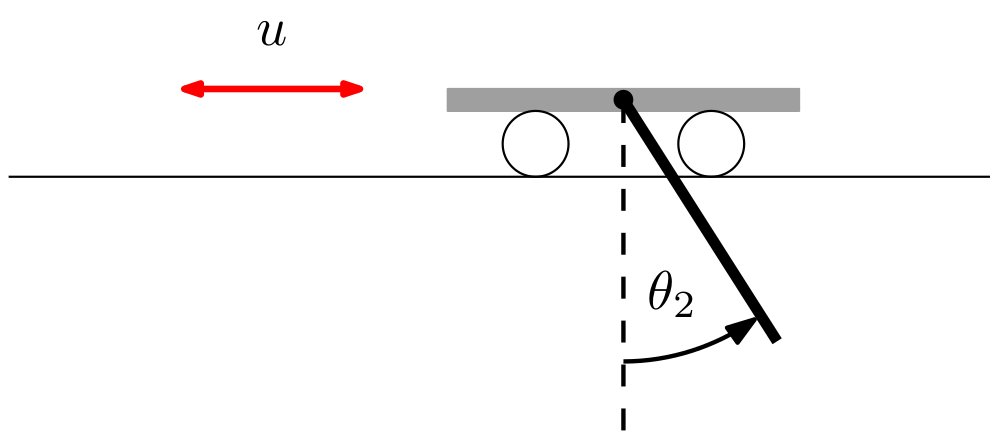
\includegraphics[width=0.7\textwidth]{Chapter3/Figures/cart-pole.png}
\caption[Cart-pole PILCO environment]{Cart-pole swing up. Source: \cite{deisenroth2013pilco-documentation}.}
\label{Fig:cartpole-environment}
\end{figure}
The system has 4 continuous state variables: the position of the cart $x$, the velocity of the cart $\dot x$, the pendulum angle $\theta_2$, and the angular velocity of the pendulum $\dot \theta_2$ of the pendulum. There is a target associated with each state variable.

\subsubsection{Pendubot}
The \textit{Pendubot}, shown in Fig. \ref{Fig:pendubot-environment}, is the second most complex environment used for experimentation. It consists of an \textit{inner} and an \textit{outer} pendulum, with masses $m_1$ and $m_2$ and lengths $l_1$ and $l_2$, respectively. The two pendulums are linked together, with the inner pendulum also being attached to the ground. The inner and outer pendulum angles are given by $\theta_2$ and $\theta_3$, respectively, measured anticlockwise from the upright vertical position. The link between the ground and the inner pendulum can be acted upon by the agent by applying a torque $u$ to the joint; however, the link between the pendulums cannot be acted upon. The objective of the system is to apply torque to the central joint in such a way as to swing both pendulums to the upright vertical position and balance them there.
\begin{figure}[htbp]
\centering    
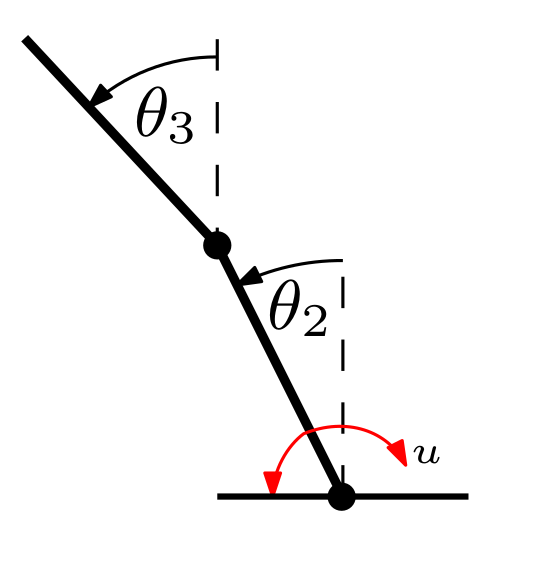
\includegraphics[width=0.3\textwidth]{Chapter3/Figures/pendubot.png}
\caption[Pendubot PILCO environment]{Source: \cite{deisenroth2013pilco-documentation}.}
\label{Fig:pendubot-environment}
\end{figure}

The system has 4 continuous state variables: the angles of the pendulums $\theta_2$ and $\theta_3$ and the angular velocities of the pendulums $\dot \theta_2$ and $\dot \theta_3$. There is a target associated with each state variable.

\subsubsection{Cart-Double-Pendulum}
The \textit{cart-double-pendulum} problem, shown in Fig. \ref{Fig:cartDoublePendulum-environment}, is the most complex environment used for experimentation. It consists of a cart of mass $m_1$, as well as an inner and an outer pendulum of masses $m_2$ and $m_3$ and lengths $l_2$ and $l_3$, respectively. The two pendulums are linked together, with the inner pendulum also being attached to the cart.  The central and outer pendulum angles are given by $\theta_2$ and $\theta_3$, respectively, and are measured anticlockwise from the upright vertical position. Continuous control actions $u$ applied to the cart cause it to move horizontally in the $x$-direction. The objective of the task is to apply horizontal force to the cart in such a way that the double pendulum system is swung to the upright vertical position and balanced there while positioning the cart in the centre of the system at $x=0$. The unconstrained double pendulum system exhibits rich dynamical behaviour and is a chaotic system.
\begin{figure}[htbp]
\centering    
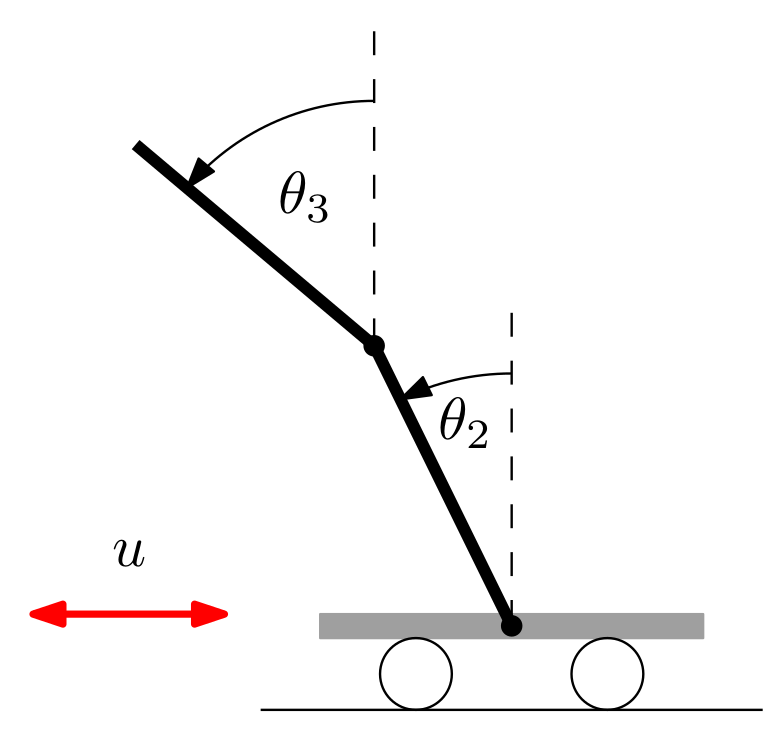
\includegraphics[width=0.4\textwidth]{Chapter3/Figures/cart-double-pendulum.png}
\caption[Cart-double-pendulum PILCO environment]{Source \cite{deisenroth2013pilco-documentation}.}
\label{Fig:cartDoublePendulum-environment}
\end{figure}

The system has 6 continuous state variables: the position of the cart $x$, the velocity of the cart $\dot x$, the angles of the pendulums $\theta_2$ and $\theta_3$ the angular velocities of the pendulums $\dot \theta_2$ and $\dot \theta_3$. There is a target associated with each state variable.


\section{Experiments}
\label{S:results}
\subsection{The Evolution of Distributions over States and Costs}
I obtain Monte Carlo uncertainty estimates by rolling out state-action values through the dynamics model using the one-step predictions given in Eq. \ref{Eq:model-posterior-one-step}. For each state visited, I calculate the cost according to Eq. \ref{Eq:PILCO-cost-function}. 

PILCO's policy search method is formulated so that the cost is computed directly (see Eq. \ref{Eq:PILCO-expected-return}) rather than via the state (although the cost is implicitly a function of the state). It is therefore important to examine how the distributions over states and costs evolve differently as they are propagated through the model, specifically in the context of the Monte Carlo method presented in Section \ref{S:monte-carlo-estimate}. I illustrate this, as shown in Fig. \ref{Fig:1-dimensional-transition-function}, by performing $9$ steps through a simplified $1$-dimensional transition function derived from the trigonometric model presented in section \ref{S:approximating-pilcos-gp}.  The transition function represents the input space $\mathbf{x}_{t}\in [-5, 5]$ and is trained on targets representing the subsequent state $\mathbf{x}_{t+1}$ rather than state differences as is done with PILCO. 

Fig. \ref{Fig:1-dimensional-transition-function} shows the predictive mean and $95\%$ confidence interval over observed state transitions as well as $4$ example functions drawn from the posterior distribution over the model weights $q(\mathbf{w})$. To illustrate the evolution of state and cost distributions for the first step through the transition function, I sample $M=1000$ sets of weights $\mathbf{w} \sim q(\mathbf{w})$ and step through $N=1000$ starting states drawn from $\mathbf{x}_{0} \sim \mathcal{U}(-5,5)$ according to Eq. \ref{Eq:model-posterior-one-step}. I repeat this process $8$ more times; but for each step, I feed the subsequent state $\mathbf{x}_{t+1}$, as predicted by Eq. \ref{Eq:model-posterior-one-step}, back into the equation as the input state $\mathbf{x}_{t}$. At each step I calculate the cost using Eq. \ref{Eq:PILCO-cost-function} with width $\sigma_{c}=1.5$ and target state $\mathbf{x}_{\text{target}}=0$. No explicit policy is used here. The experiment can be viewed as if there is only one action and the agent selects that action at each opportunity. This enables states and costs to evolve freely under the system dynamics.

\begin{figure}[htbp]
\centering    
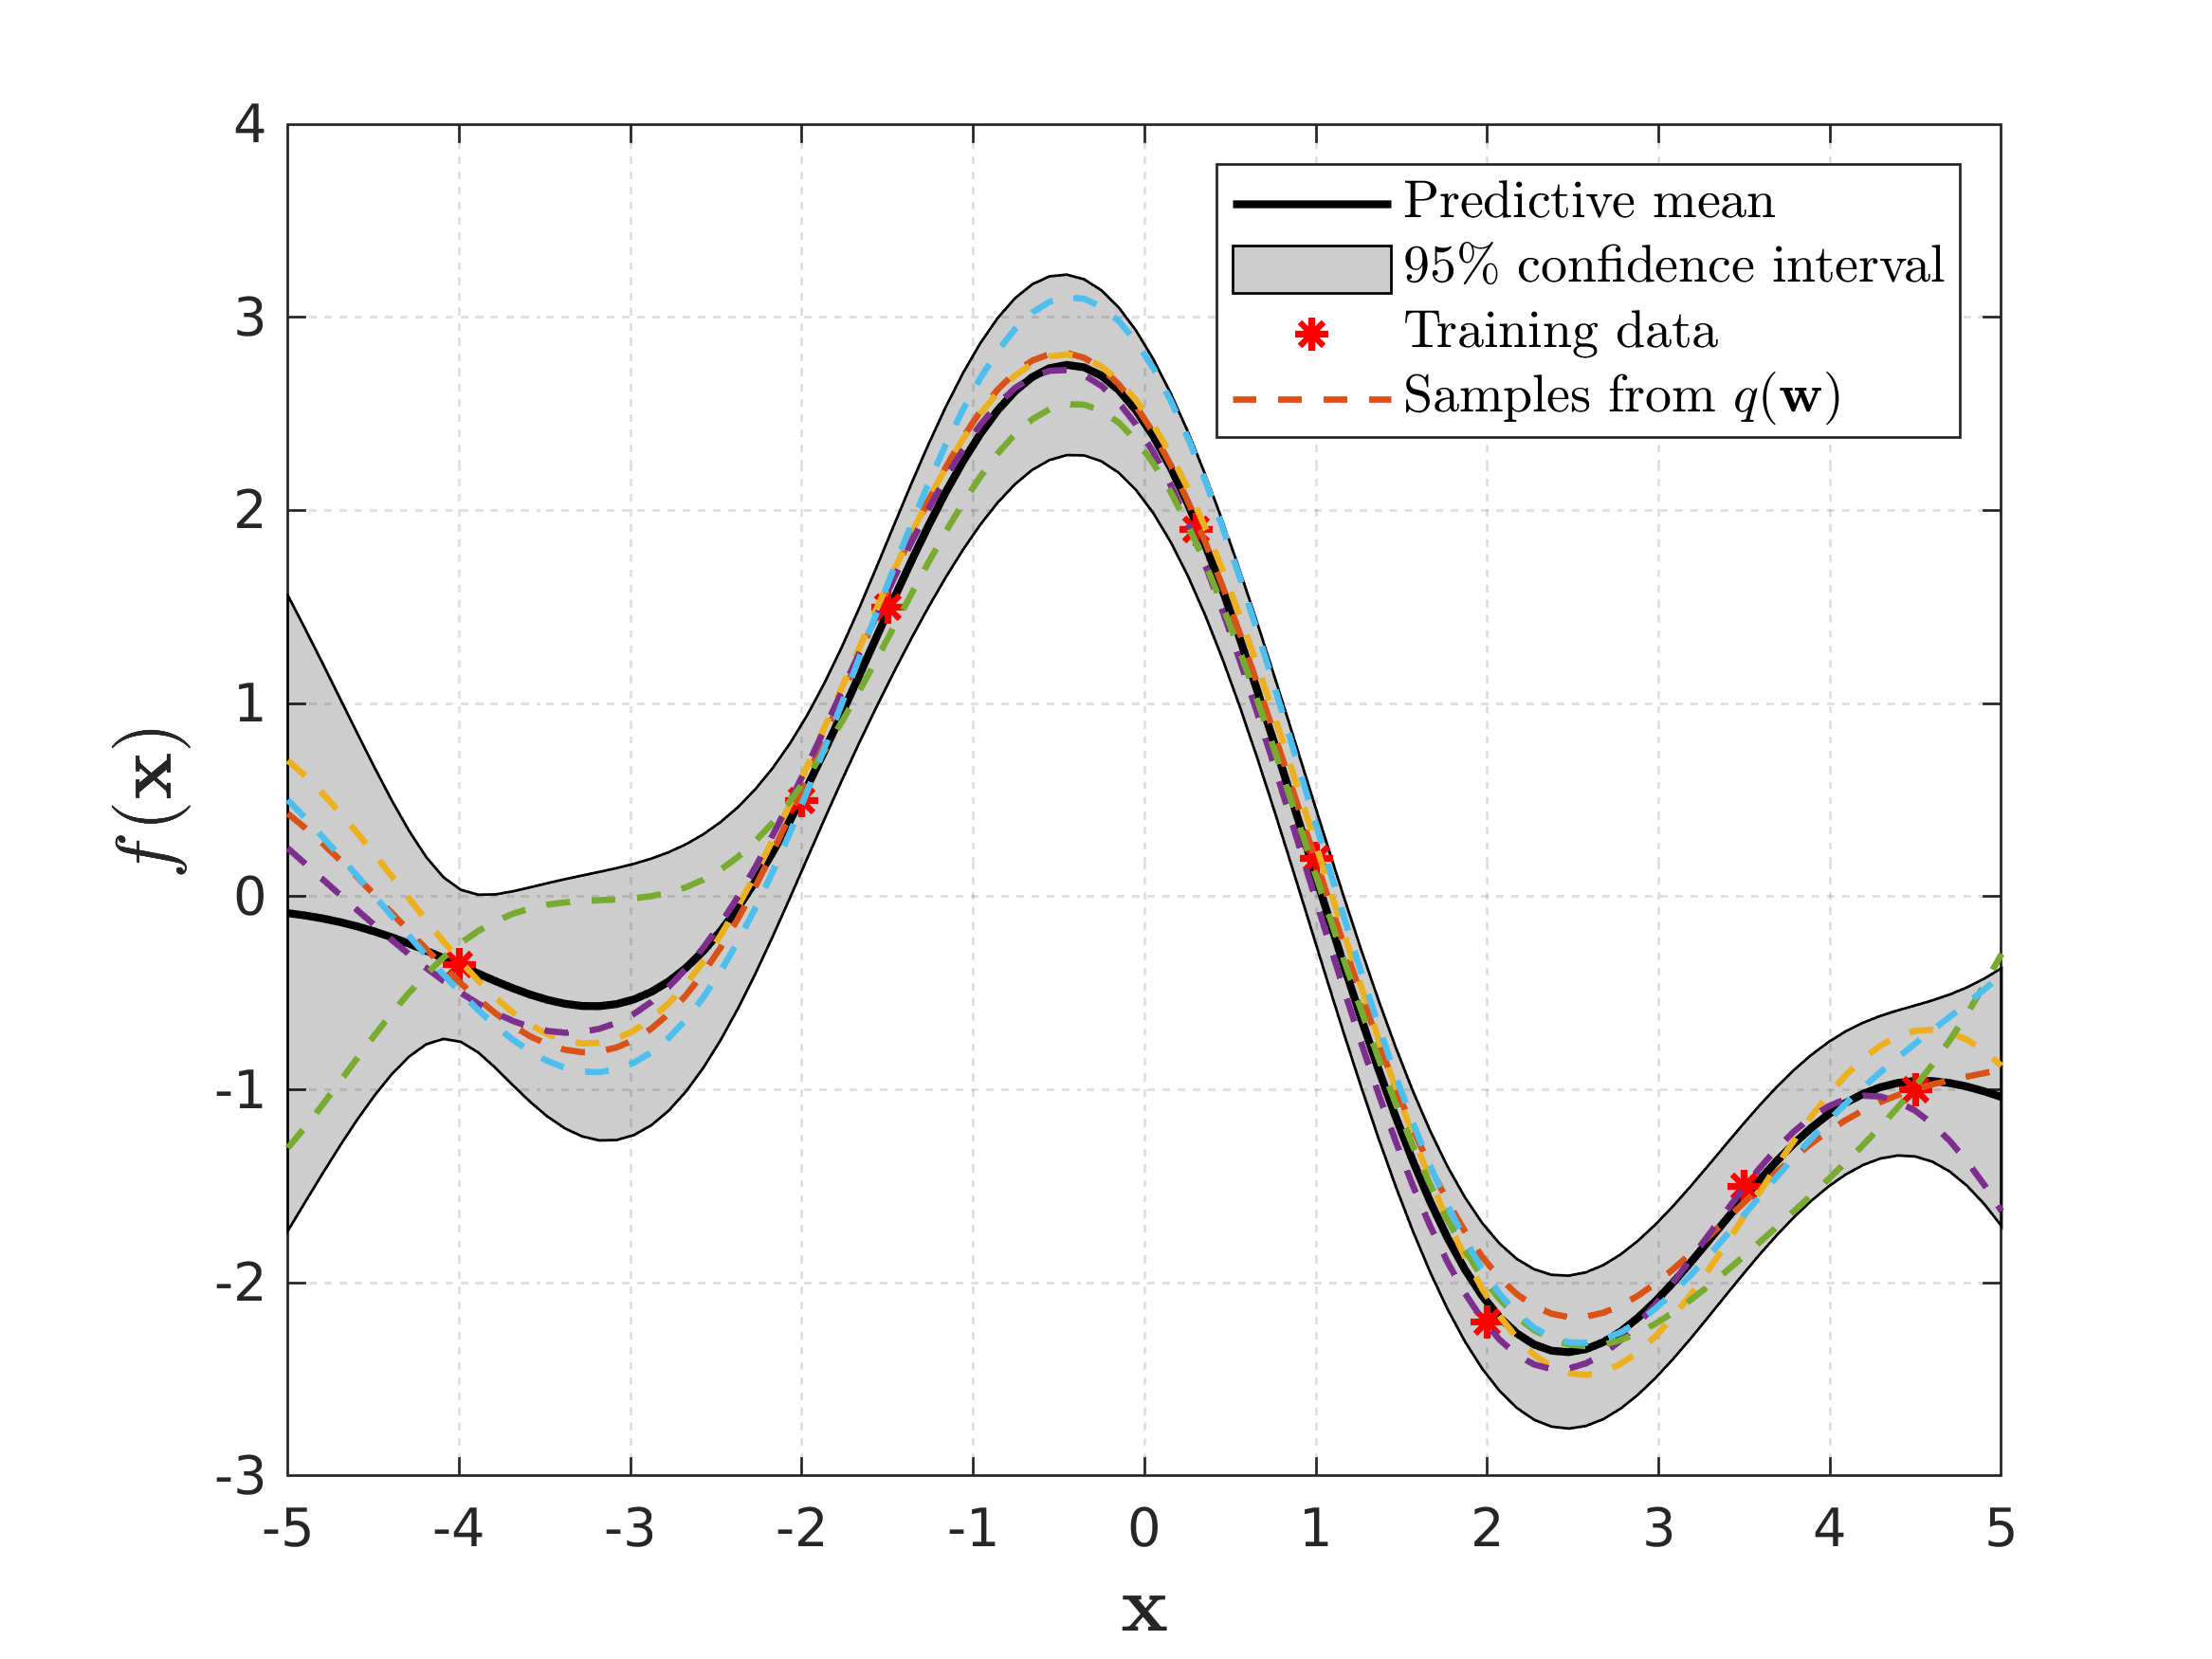
\includegraphics[width=0.6\textwidth]{Chapter3/Figures/transition_function.png}
\caption[Example: 1-dimensional transition function]{A 1-dimensional transition function example}
\label{Fig:1-dimensional-transition-function}
\end{figure}

Fig \ref{Fig:Re-evolution-of-state-and-cost} shows the evolution of the distributions over states and costs. Panels \ref{Fig:Re-hist-traj-1} and \ref{Fig:Re-hist-cost-1} show the input distributions; panels \ref{Fig:Re-hist-traj-2} and \ref{Fig:Re-hist-cost-2} show the distributions after 1 transition; and panels \ref{Fig:Re-hist-traj-4} and \ref{Fig:Re-hist-cost-4} show the distributions after 9 transitions through the transition function shown in Fig. \ref{Fig:1-dimensional-transition-function}. The distribution over costs associated with the uniform initial distribution over states reveals the locally quadratic nature of the cost function where the high density at $\mathbb{C}(x)=1$ indicates saturation of costs associated with states further away from the target state. After the first step, the distribution over states tightens around the target state with a peak about $\mathbf{x}=-1$. The reduction in the state distribution tails means that the cost no longer saturates and the tightening around the target state has increased the cost density in the region of $\mathbb{C}(\mathbf{x})=0$. Finally, after 9 steps, the state distribution flattens out with small peaks around the $\pm\mathbf{x}=2$. The high density around $\mathbb{C}(x)=0$ reduces and a bump forms around the $\mathbb{C}(x)=0.8$ position corresponding to the peaks of the state distribution at about $\pm\mathbf{x}=2$. 
\begin{figure}[htbp]    
\begin{subfigure}[b]{0.48\linewidth}
    \centering
    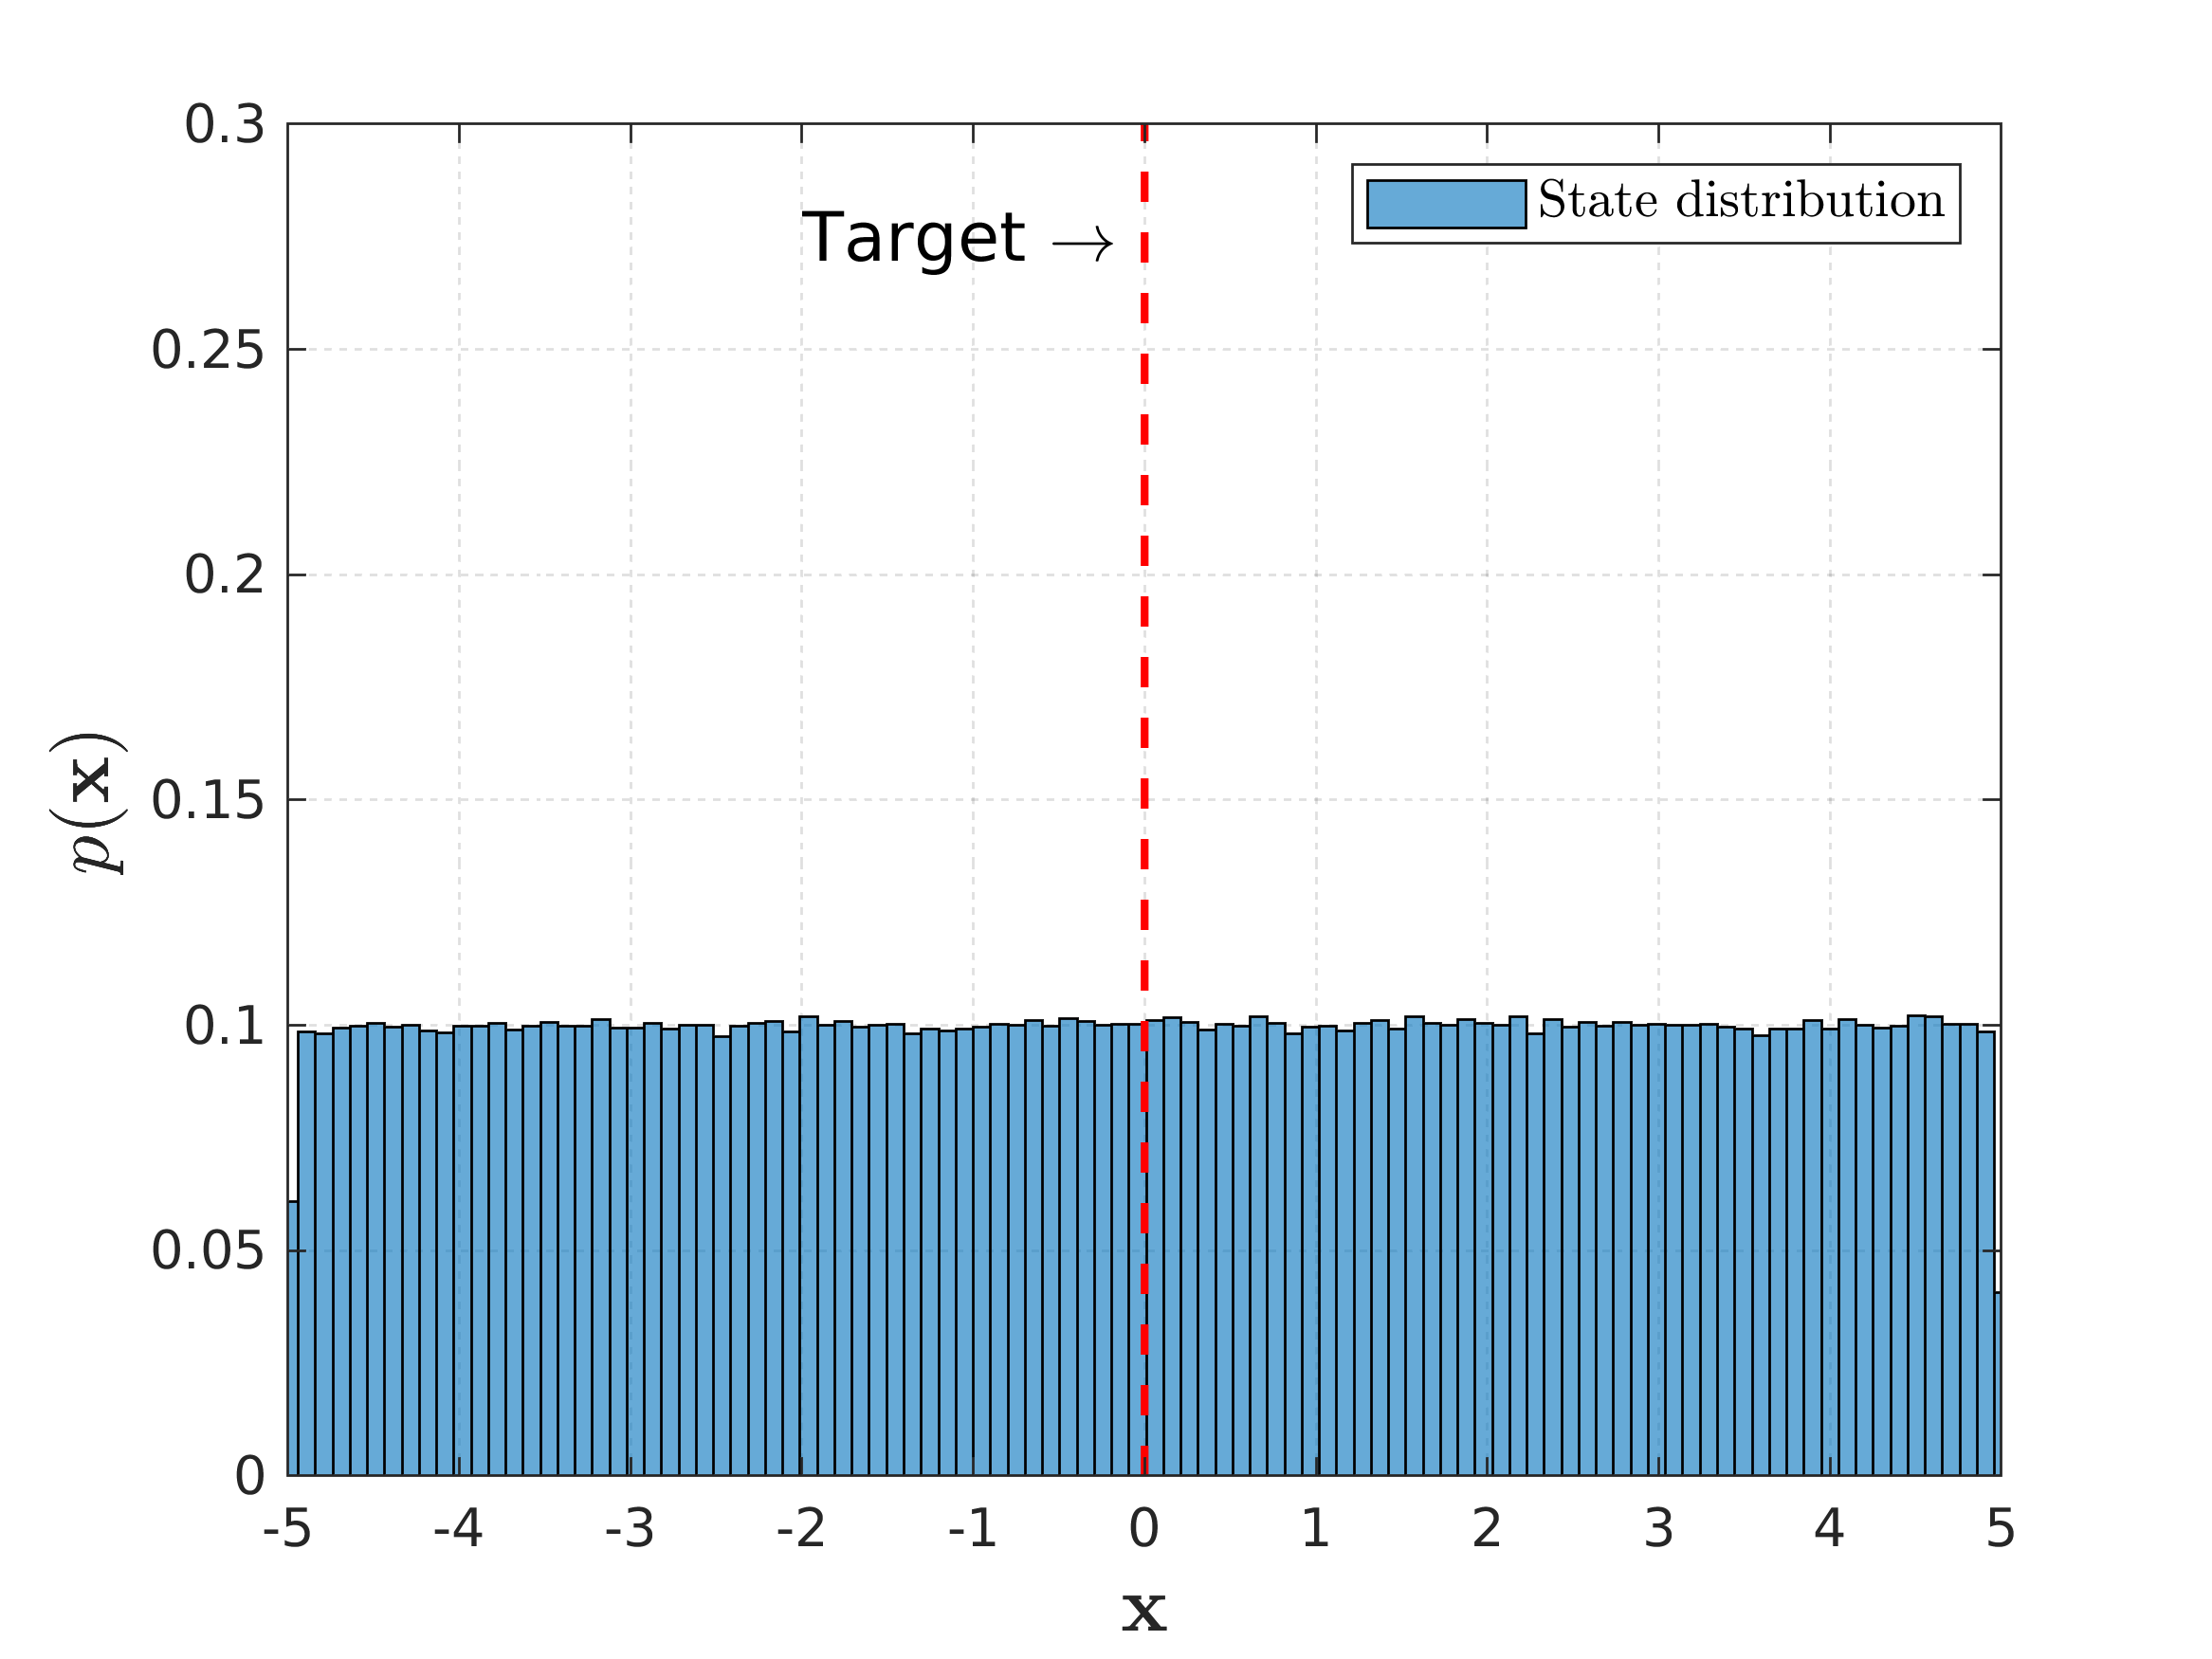
\includegraphics[height=0.22\textheight,width=0.95\textwidth]{Chapter3/Figures/trans_traj_hist_1.png} 
    \caption{Input distribution over states} 
    \label{Fig:Re-hist-traj-1} 
  \end{subfigure} 
  \hspace{\fill}  %% maximize space between adjacent subfigures
  \begin{subfigure}[b]{0.48\linewidth}
    \centering
    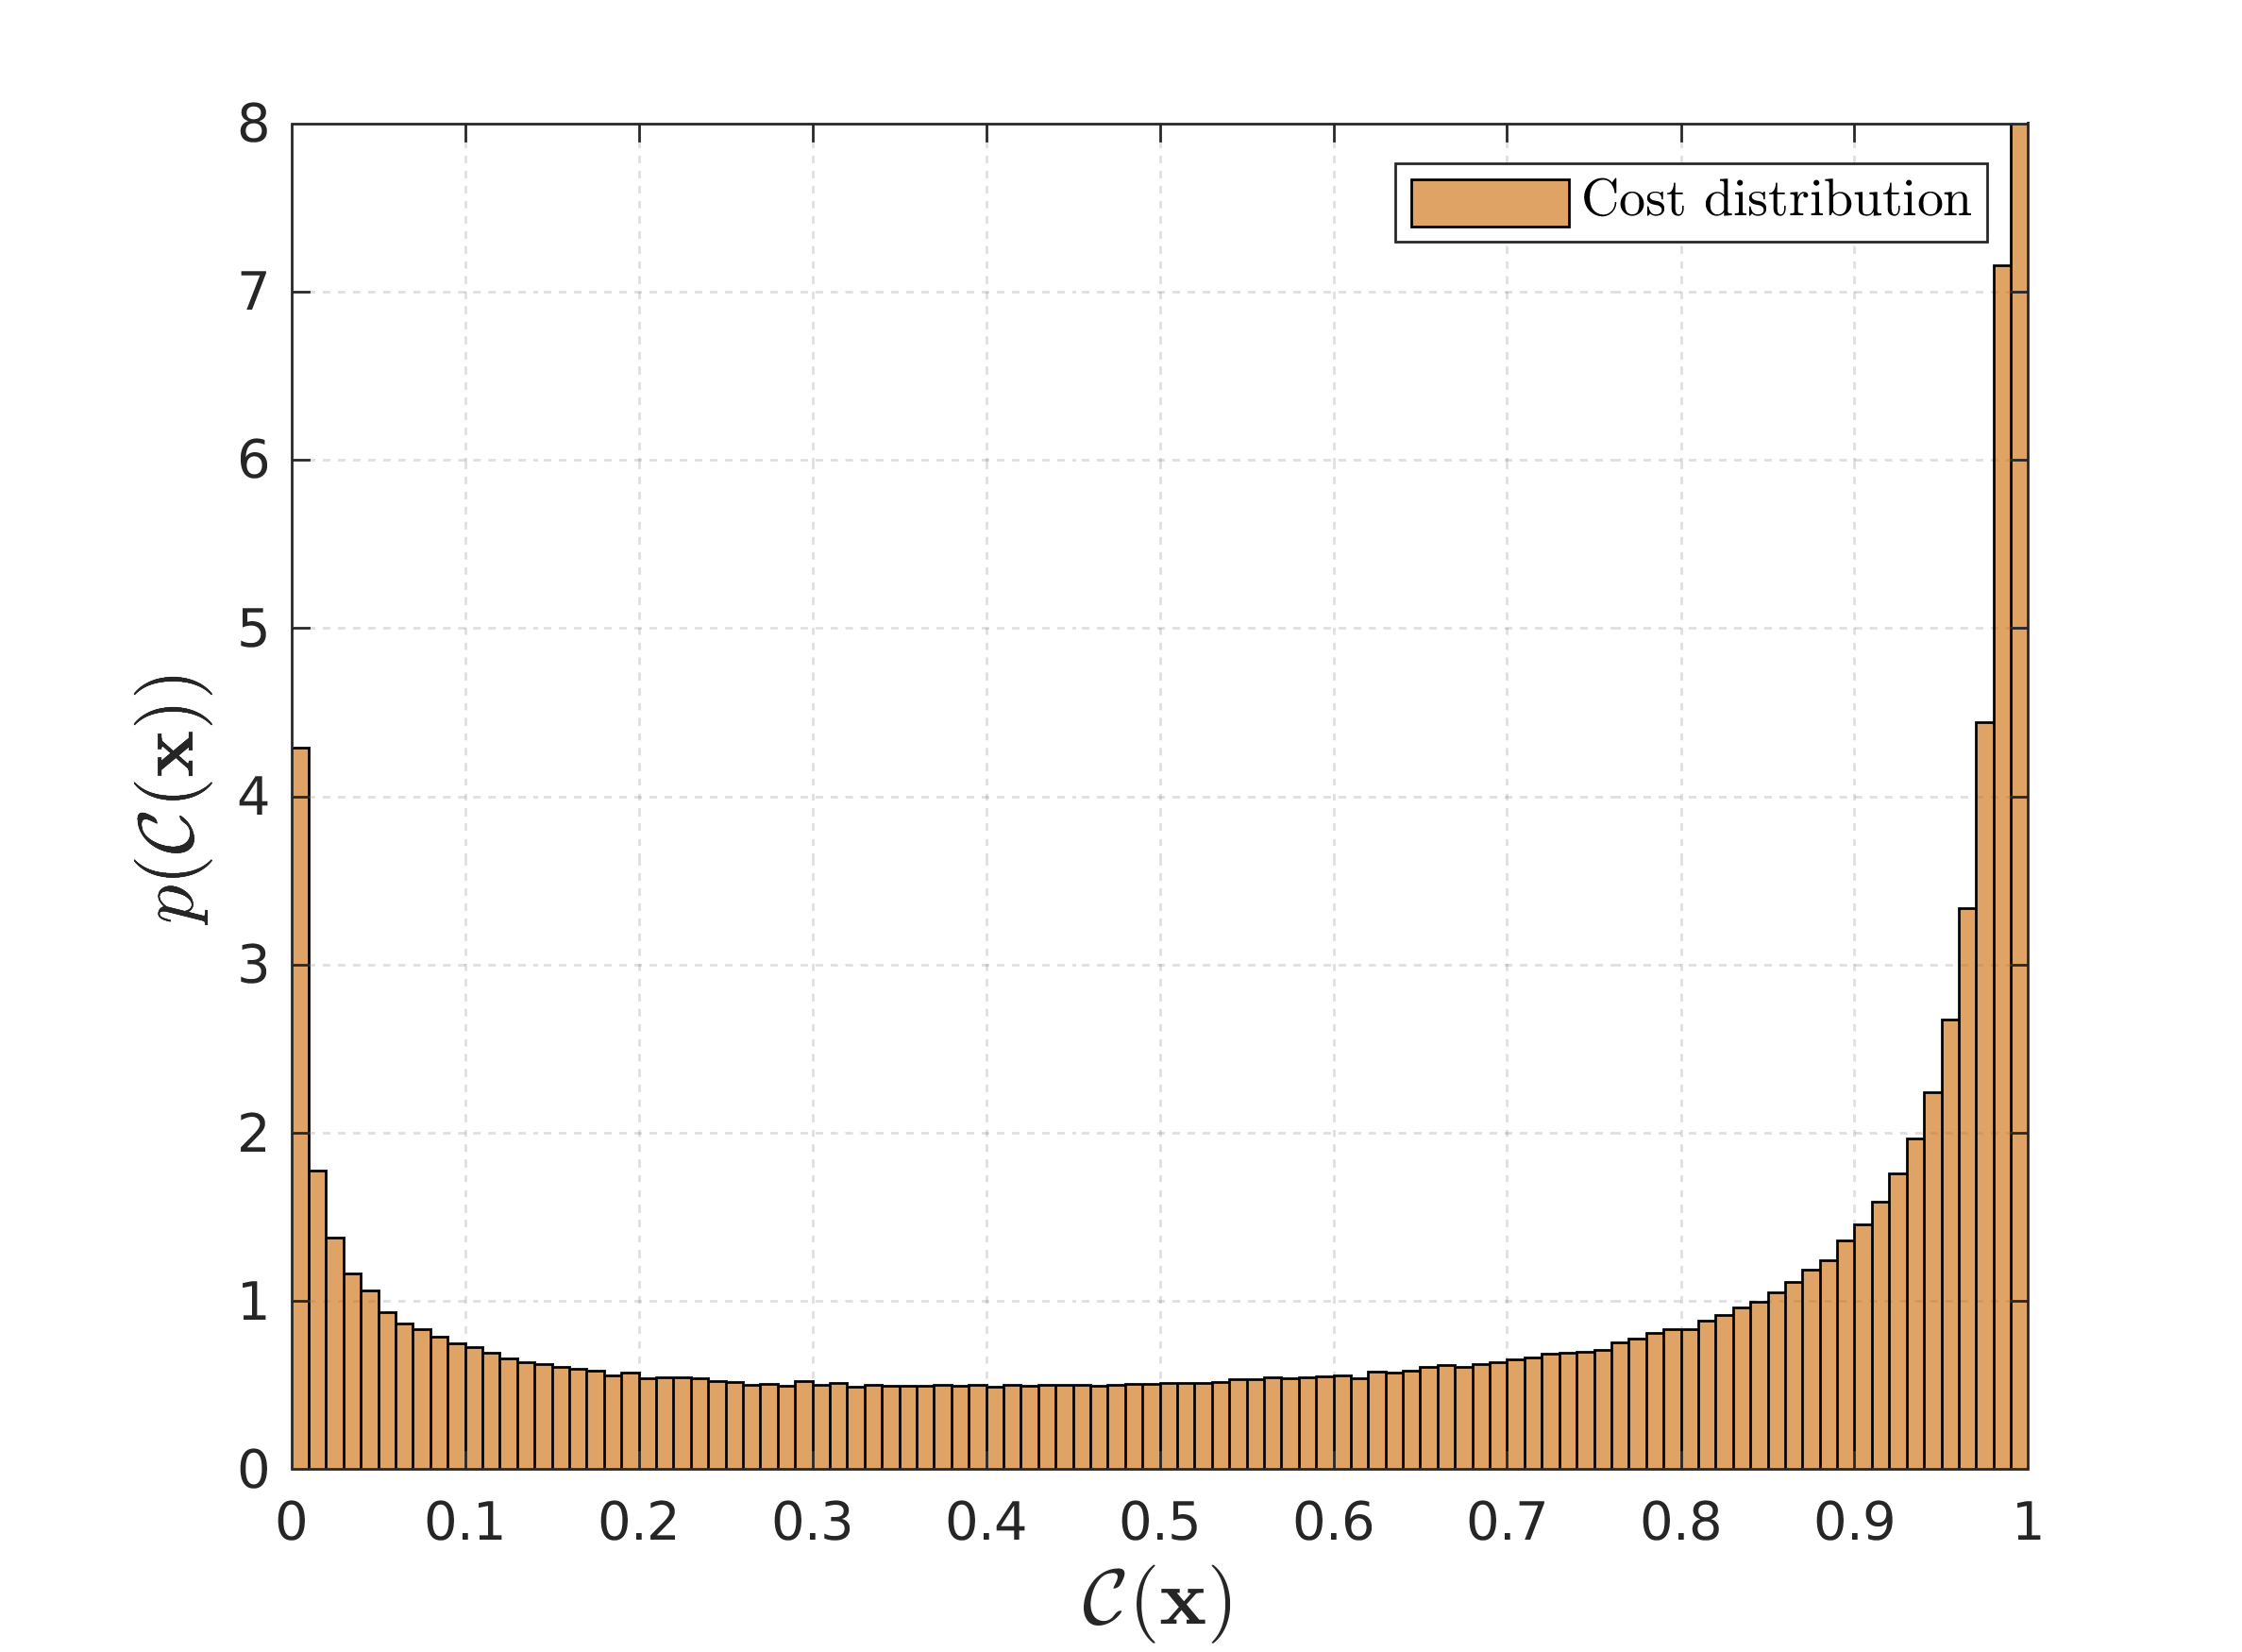
\includegraphics[height=0.22\textheight,width=0.95\textwidth]{Chapter3/Figures/trans_cost_hist_1.png} 
    \caption{Input distribution over costs} 
    \label{Fig:Re-hist-cost-1} 
  \end{subfigure} 

  \vspace{4ex}  %% extra vertical space
  \begin{subfigure}[b]{0.48\linewidth}
    \centering
    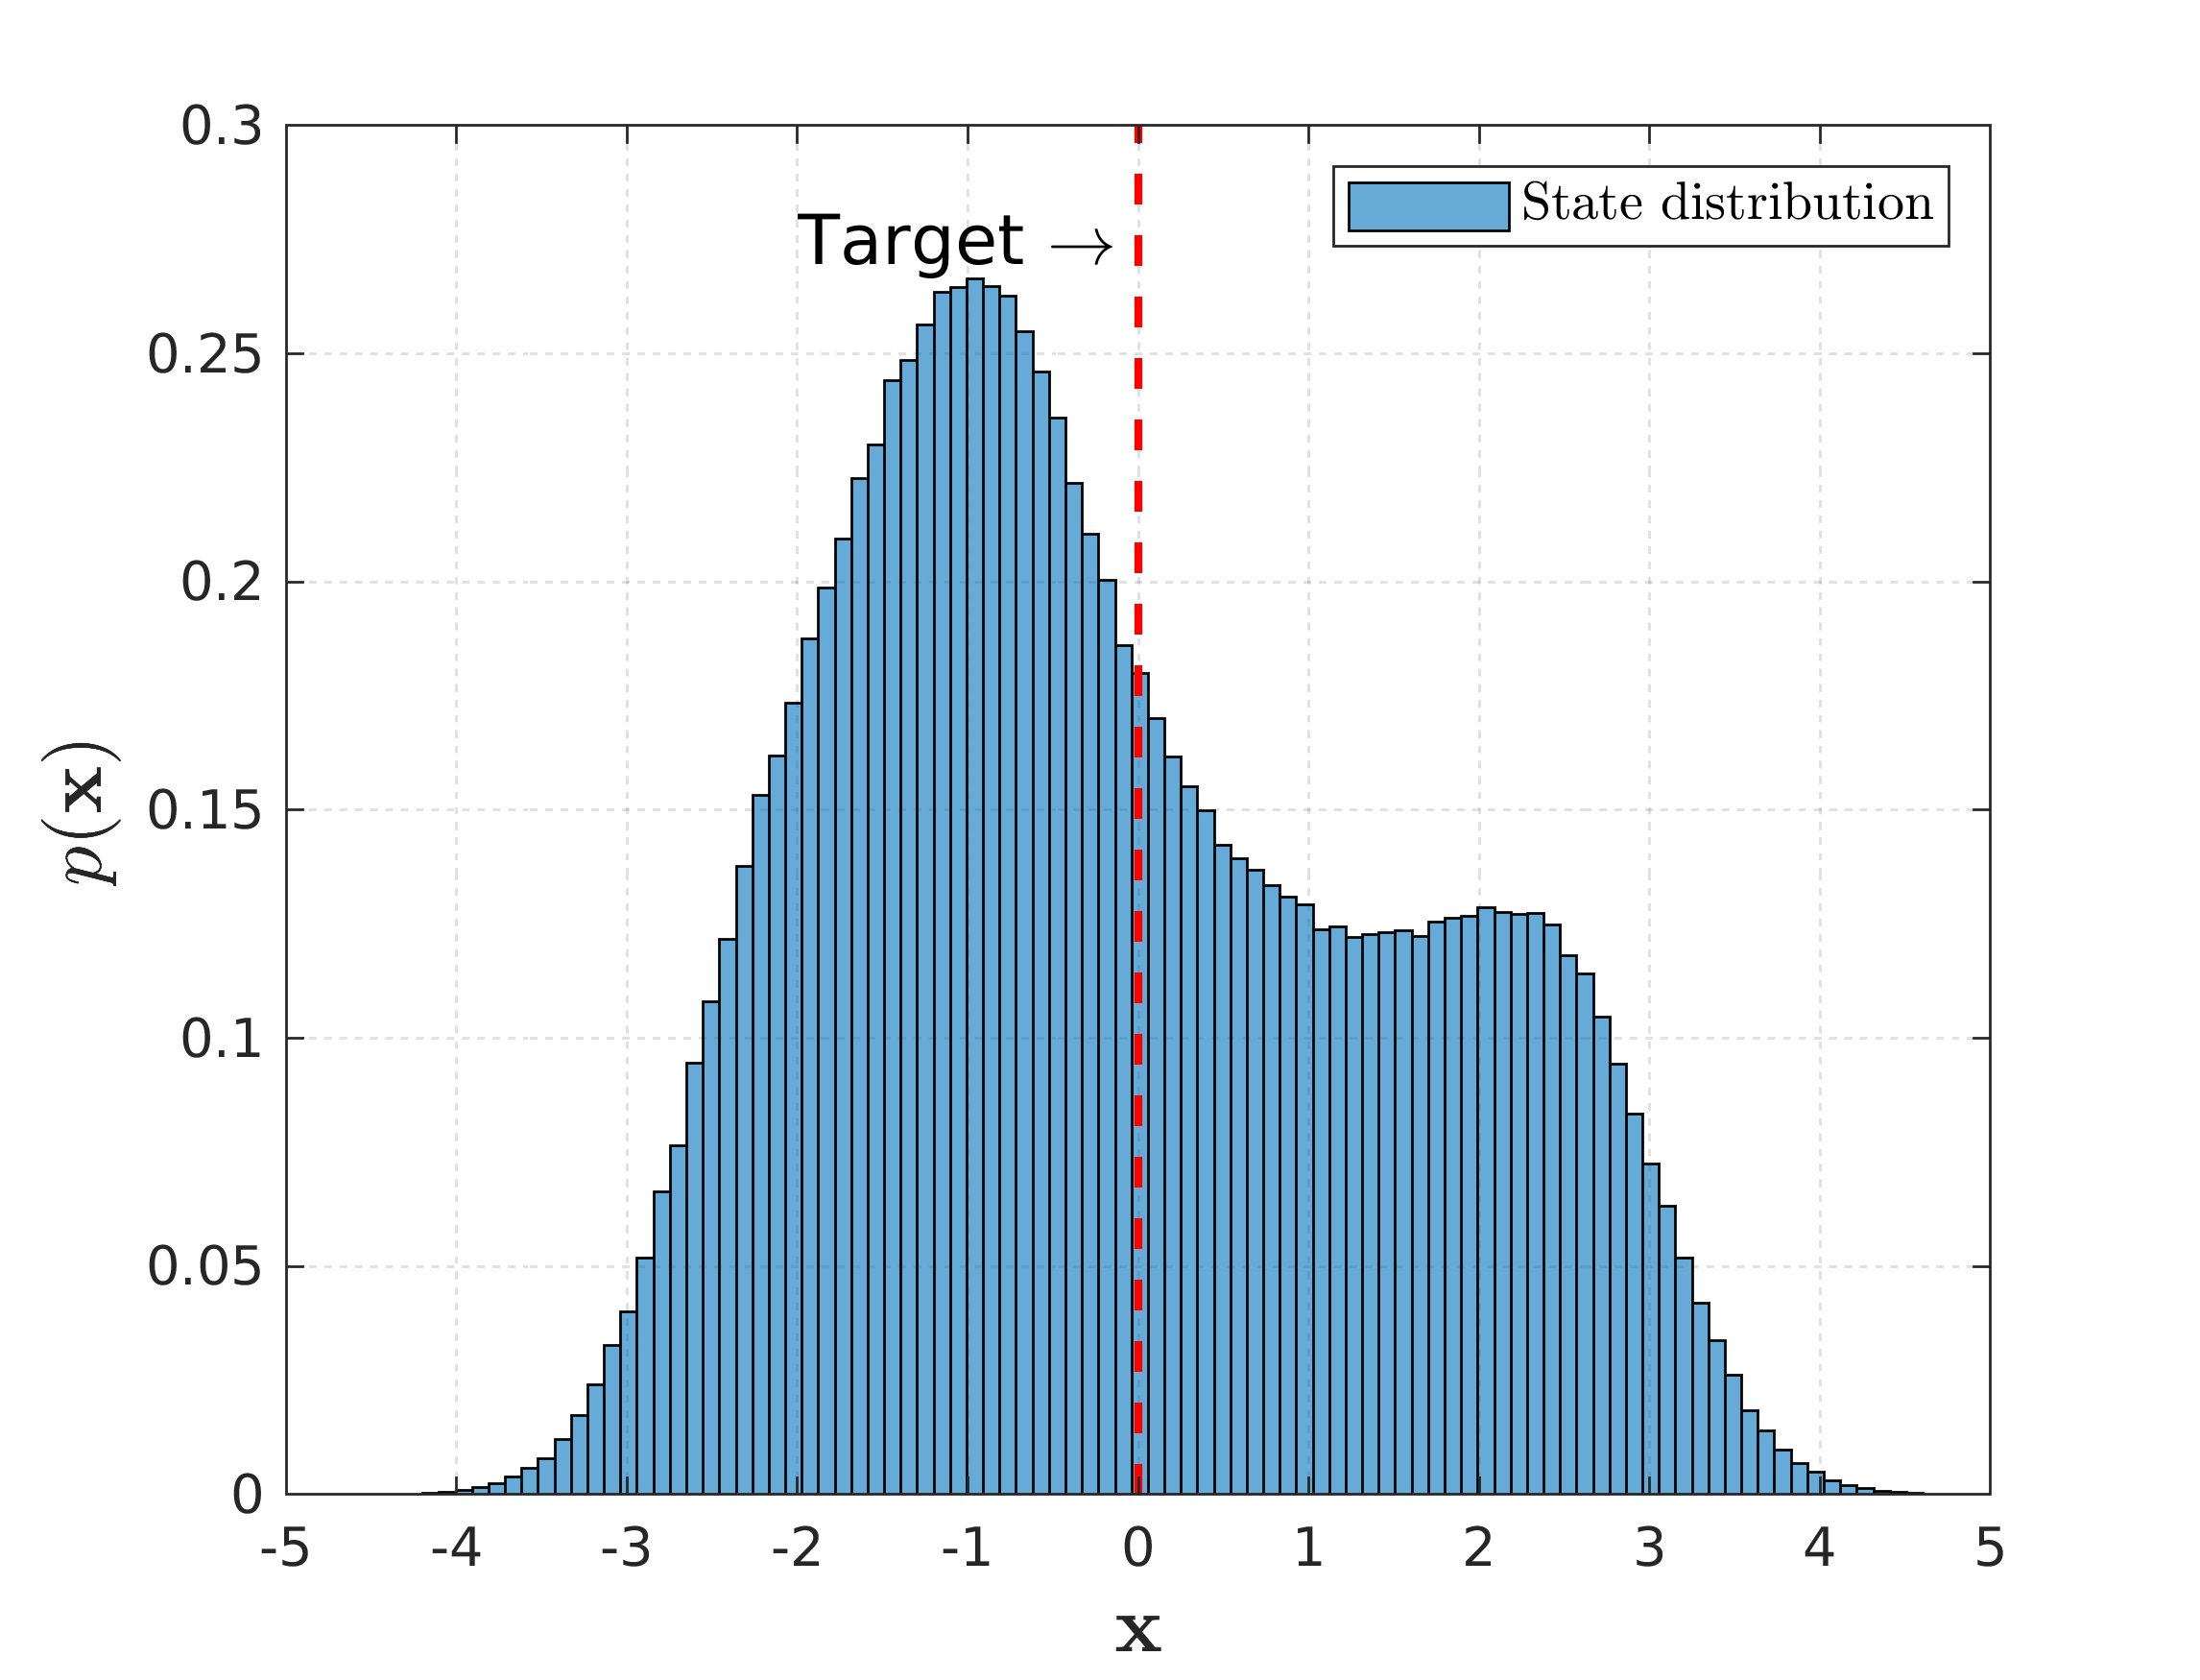
\includegraphics[height=0.22\textheight,width=0.95\textwidth]{Chapter3/Figures/trans_traj_hist_2.png} 
    \caption{Distribution over states after 1 transition} 
    \label{Fig:Re-hist-traj-2} 
  \end{subfigure} 
  \hspace{\fill}
  \begin{subfigure}[b]{0.48\linewidth}
    \centering
    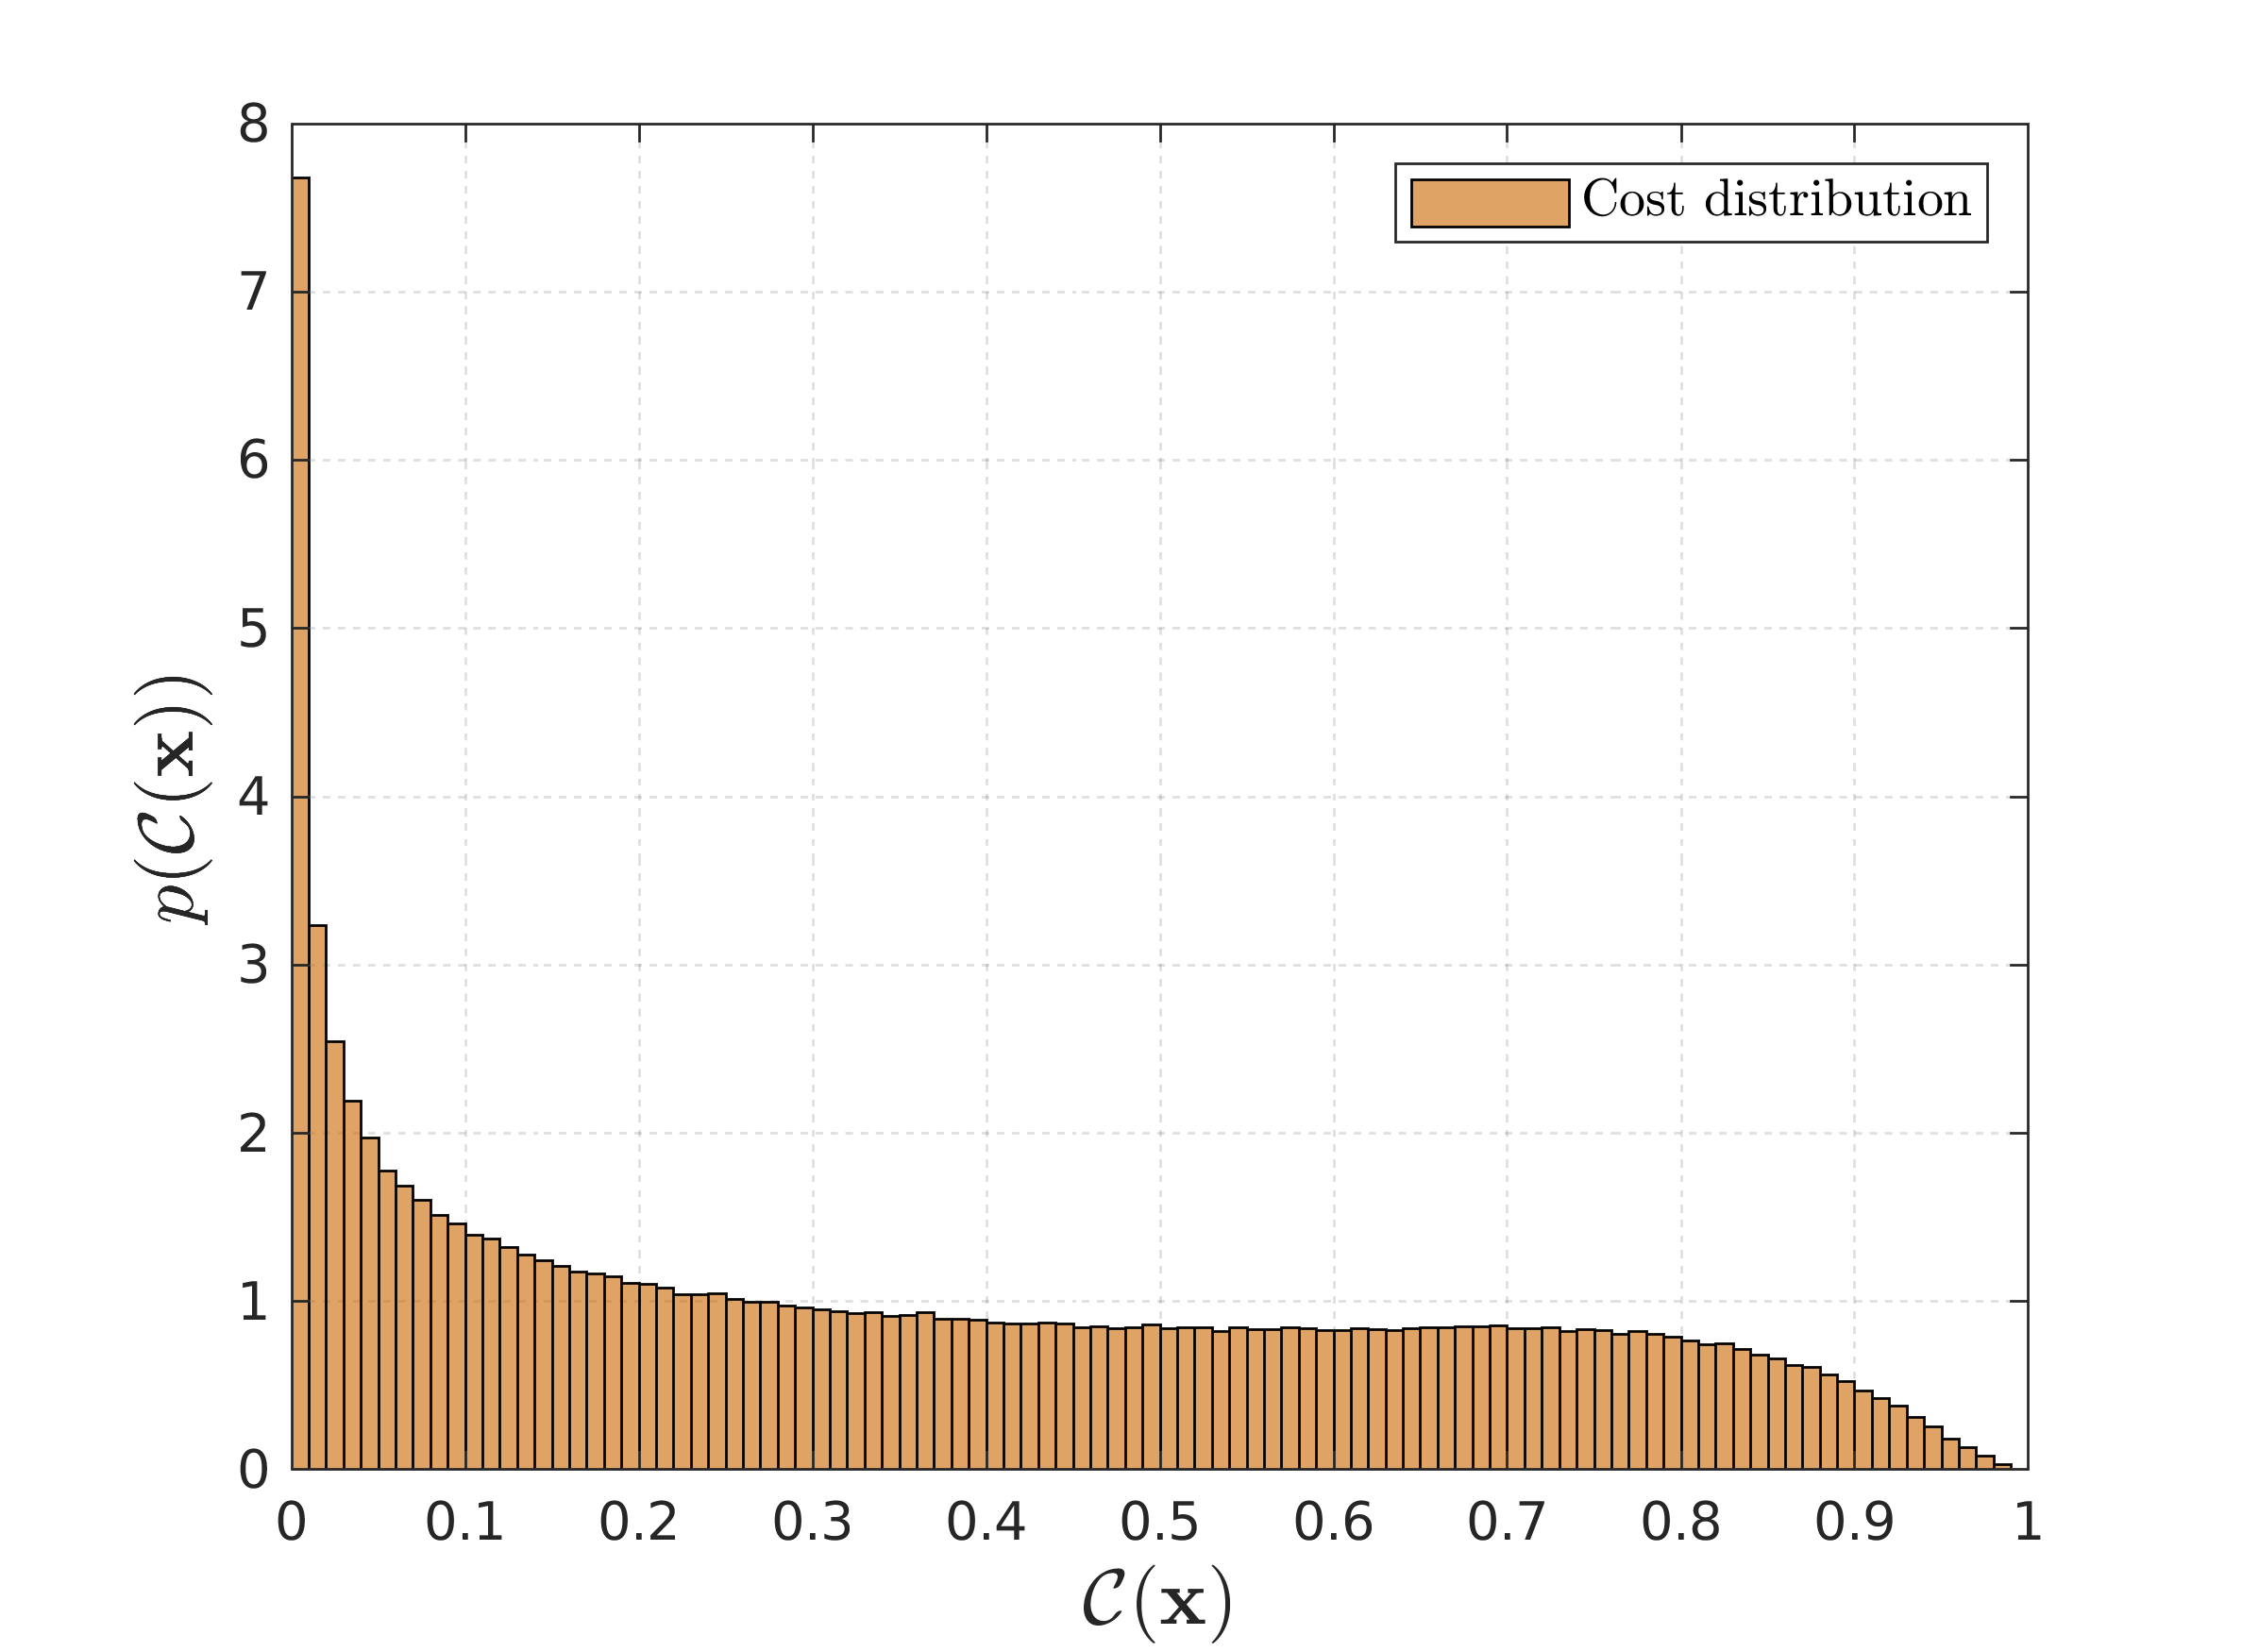
\includegraphics[height=0.22\textheight,width=0.95\textwidth]{Chapter3/Figures/trans_cost_hist_2.png} 
    \caption{Distribution over costs after 1 transition} 
    \label{Fig:Re-hist-cost-2} 
  \end{subfigure} 

    \vspace{4ex}
  \begin{subfigure}[b]{0.48\linewidth}
    \centering
    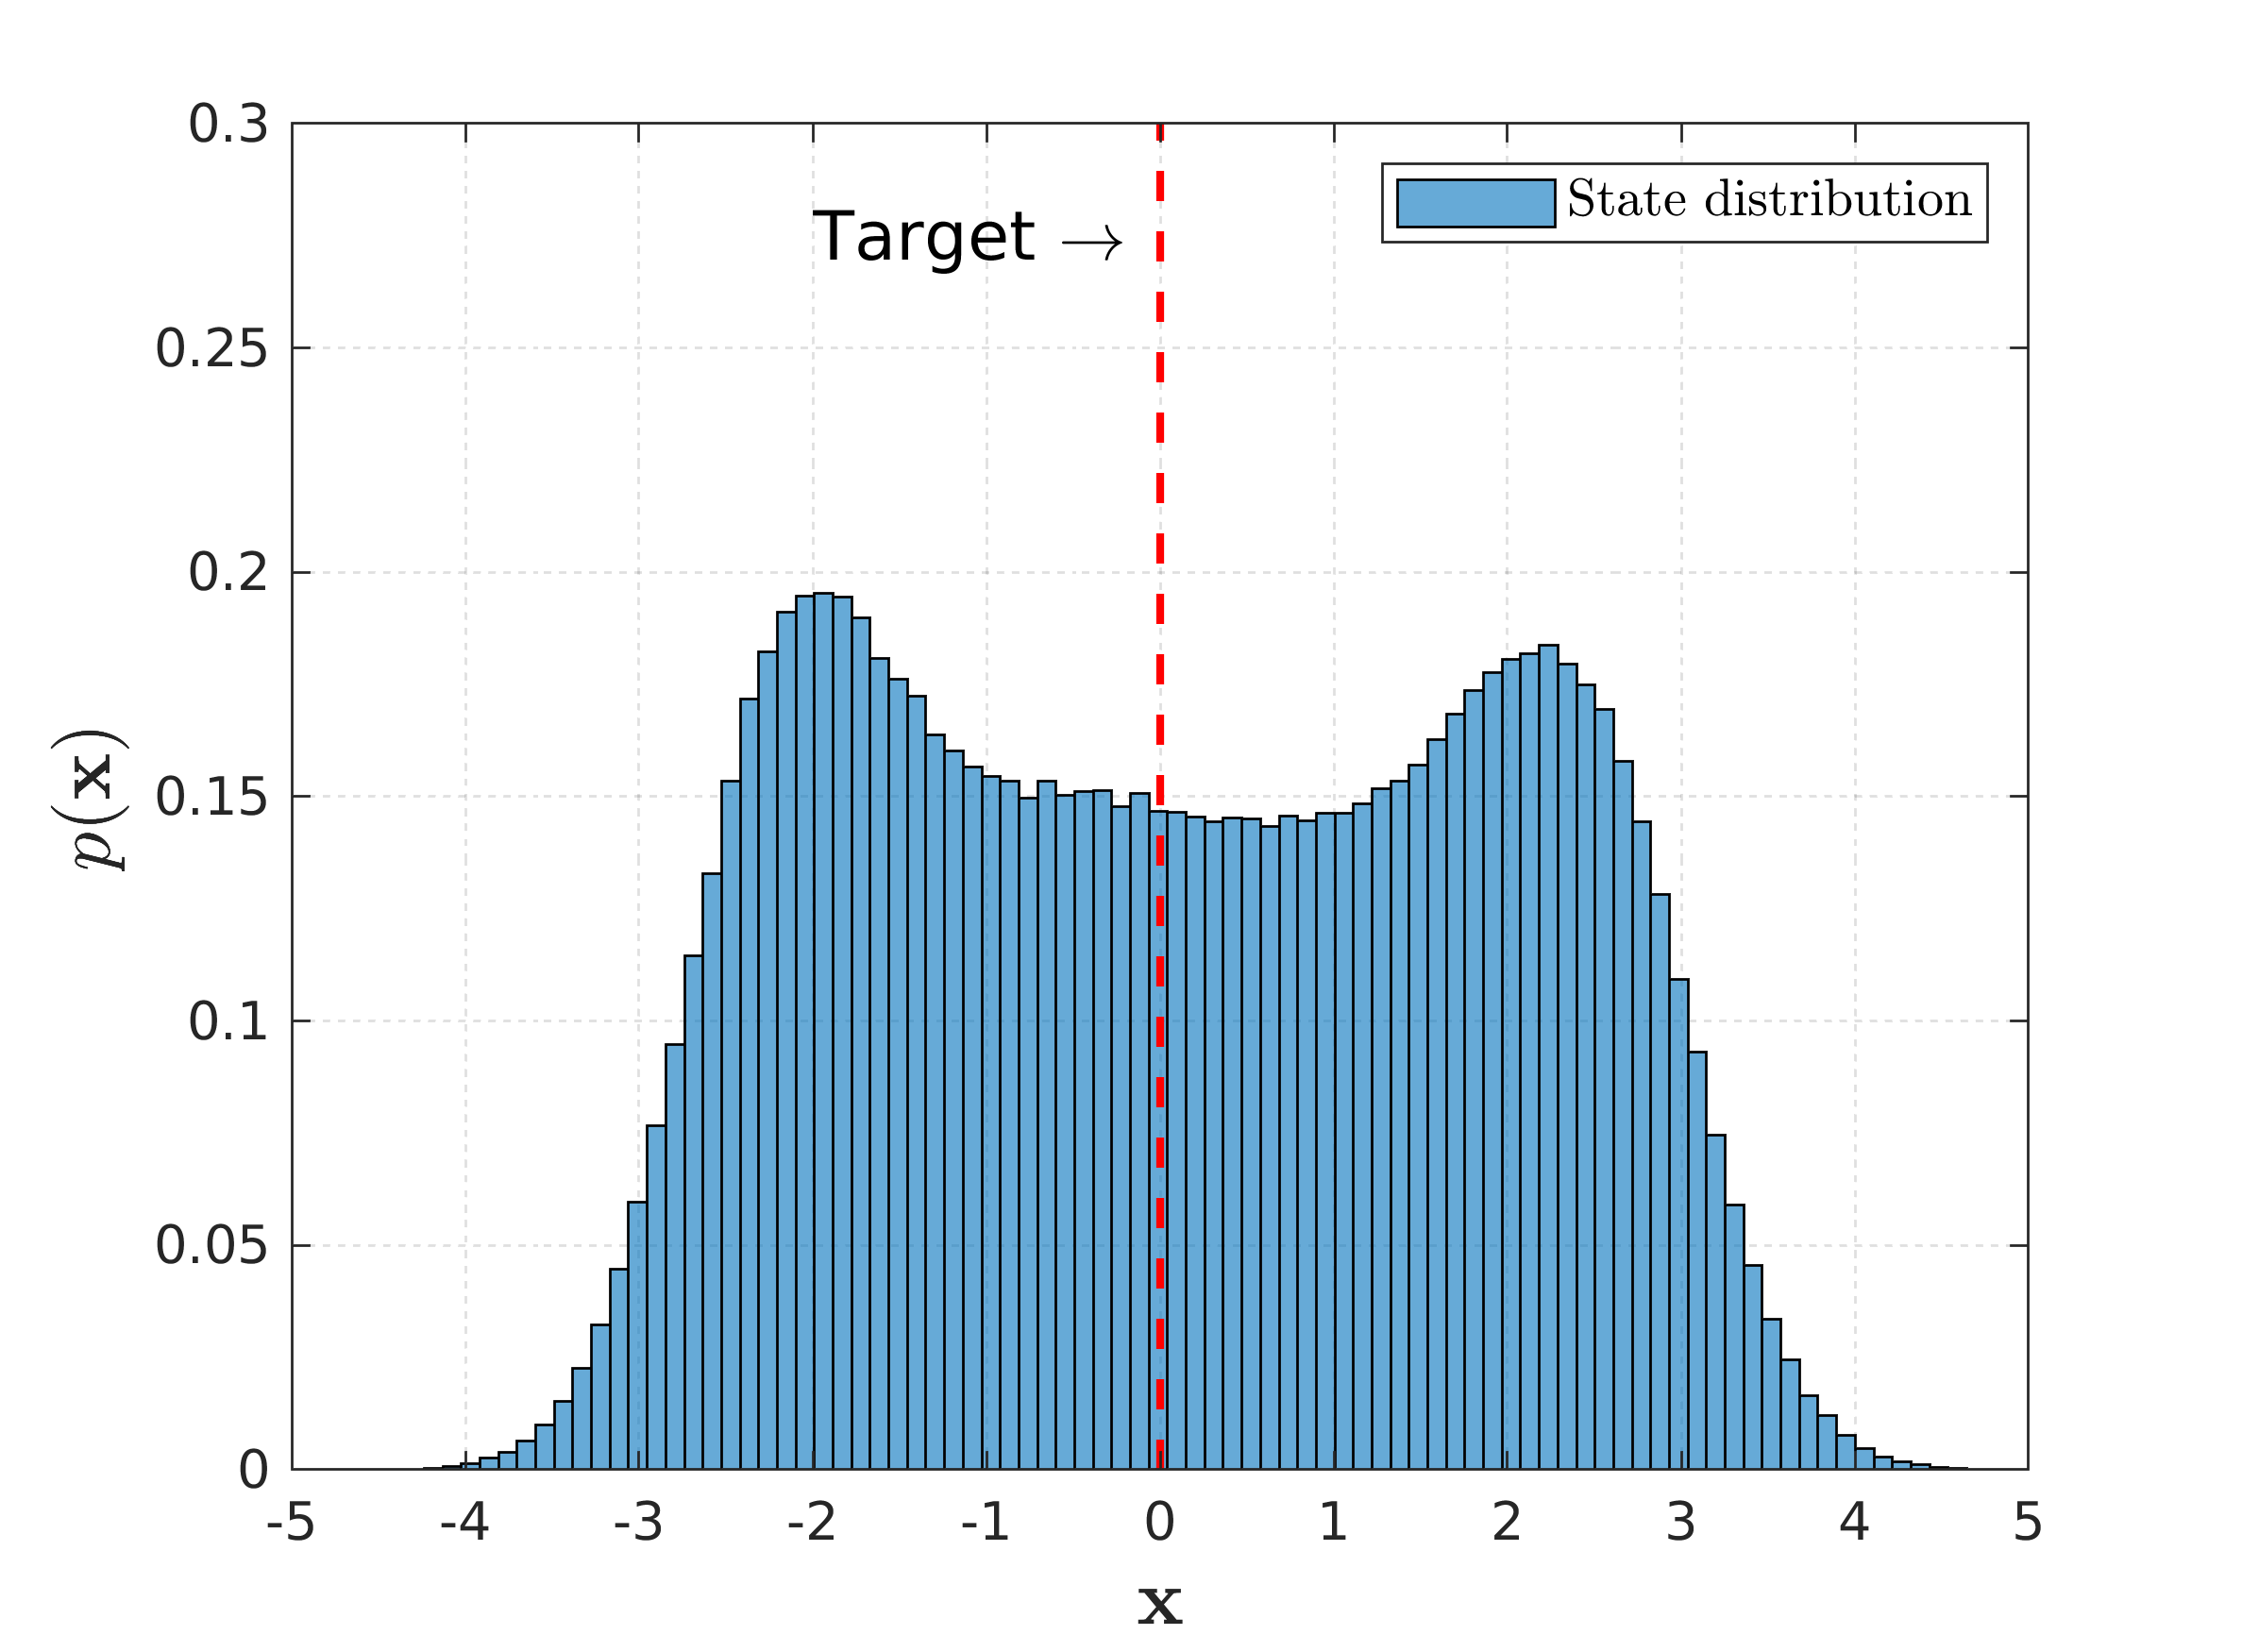
\includegraphics[height=0.22\textheight,width=0.95\textwidth]{Chapter3/Figures/trans_traj_hist_4.png} 
    \caption{Distribution over states after 9 transitions} 
    \label{Fig:Re-hist-traj-4} 
  \end{subfigure}
  \hspace{\fill}
  \begin{subfigure}[b]{0.48\linewidth}
    \centering
    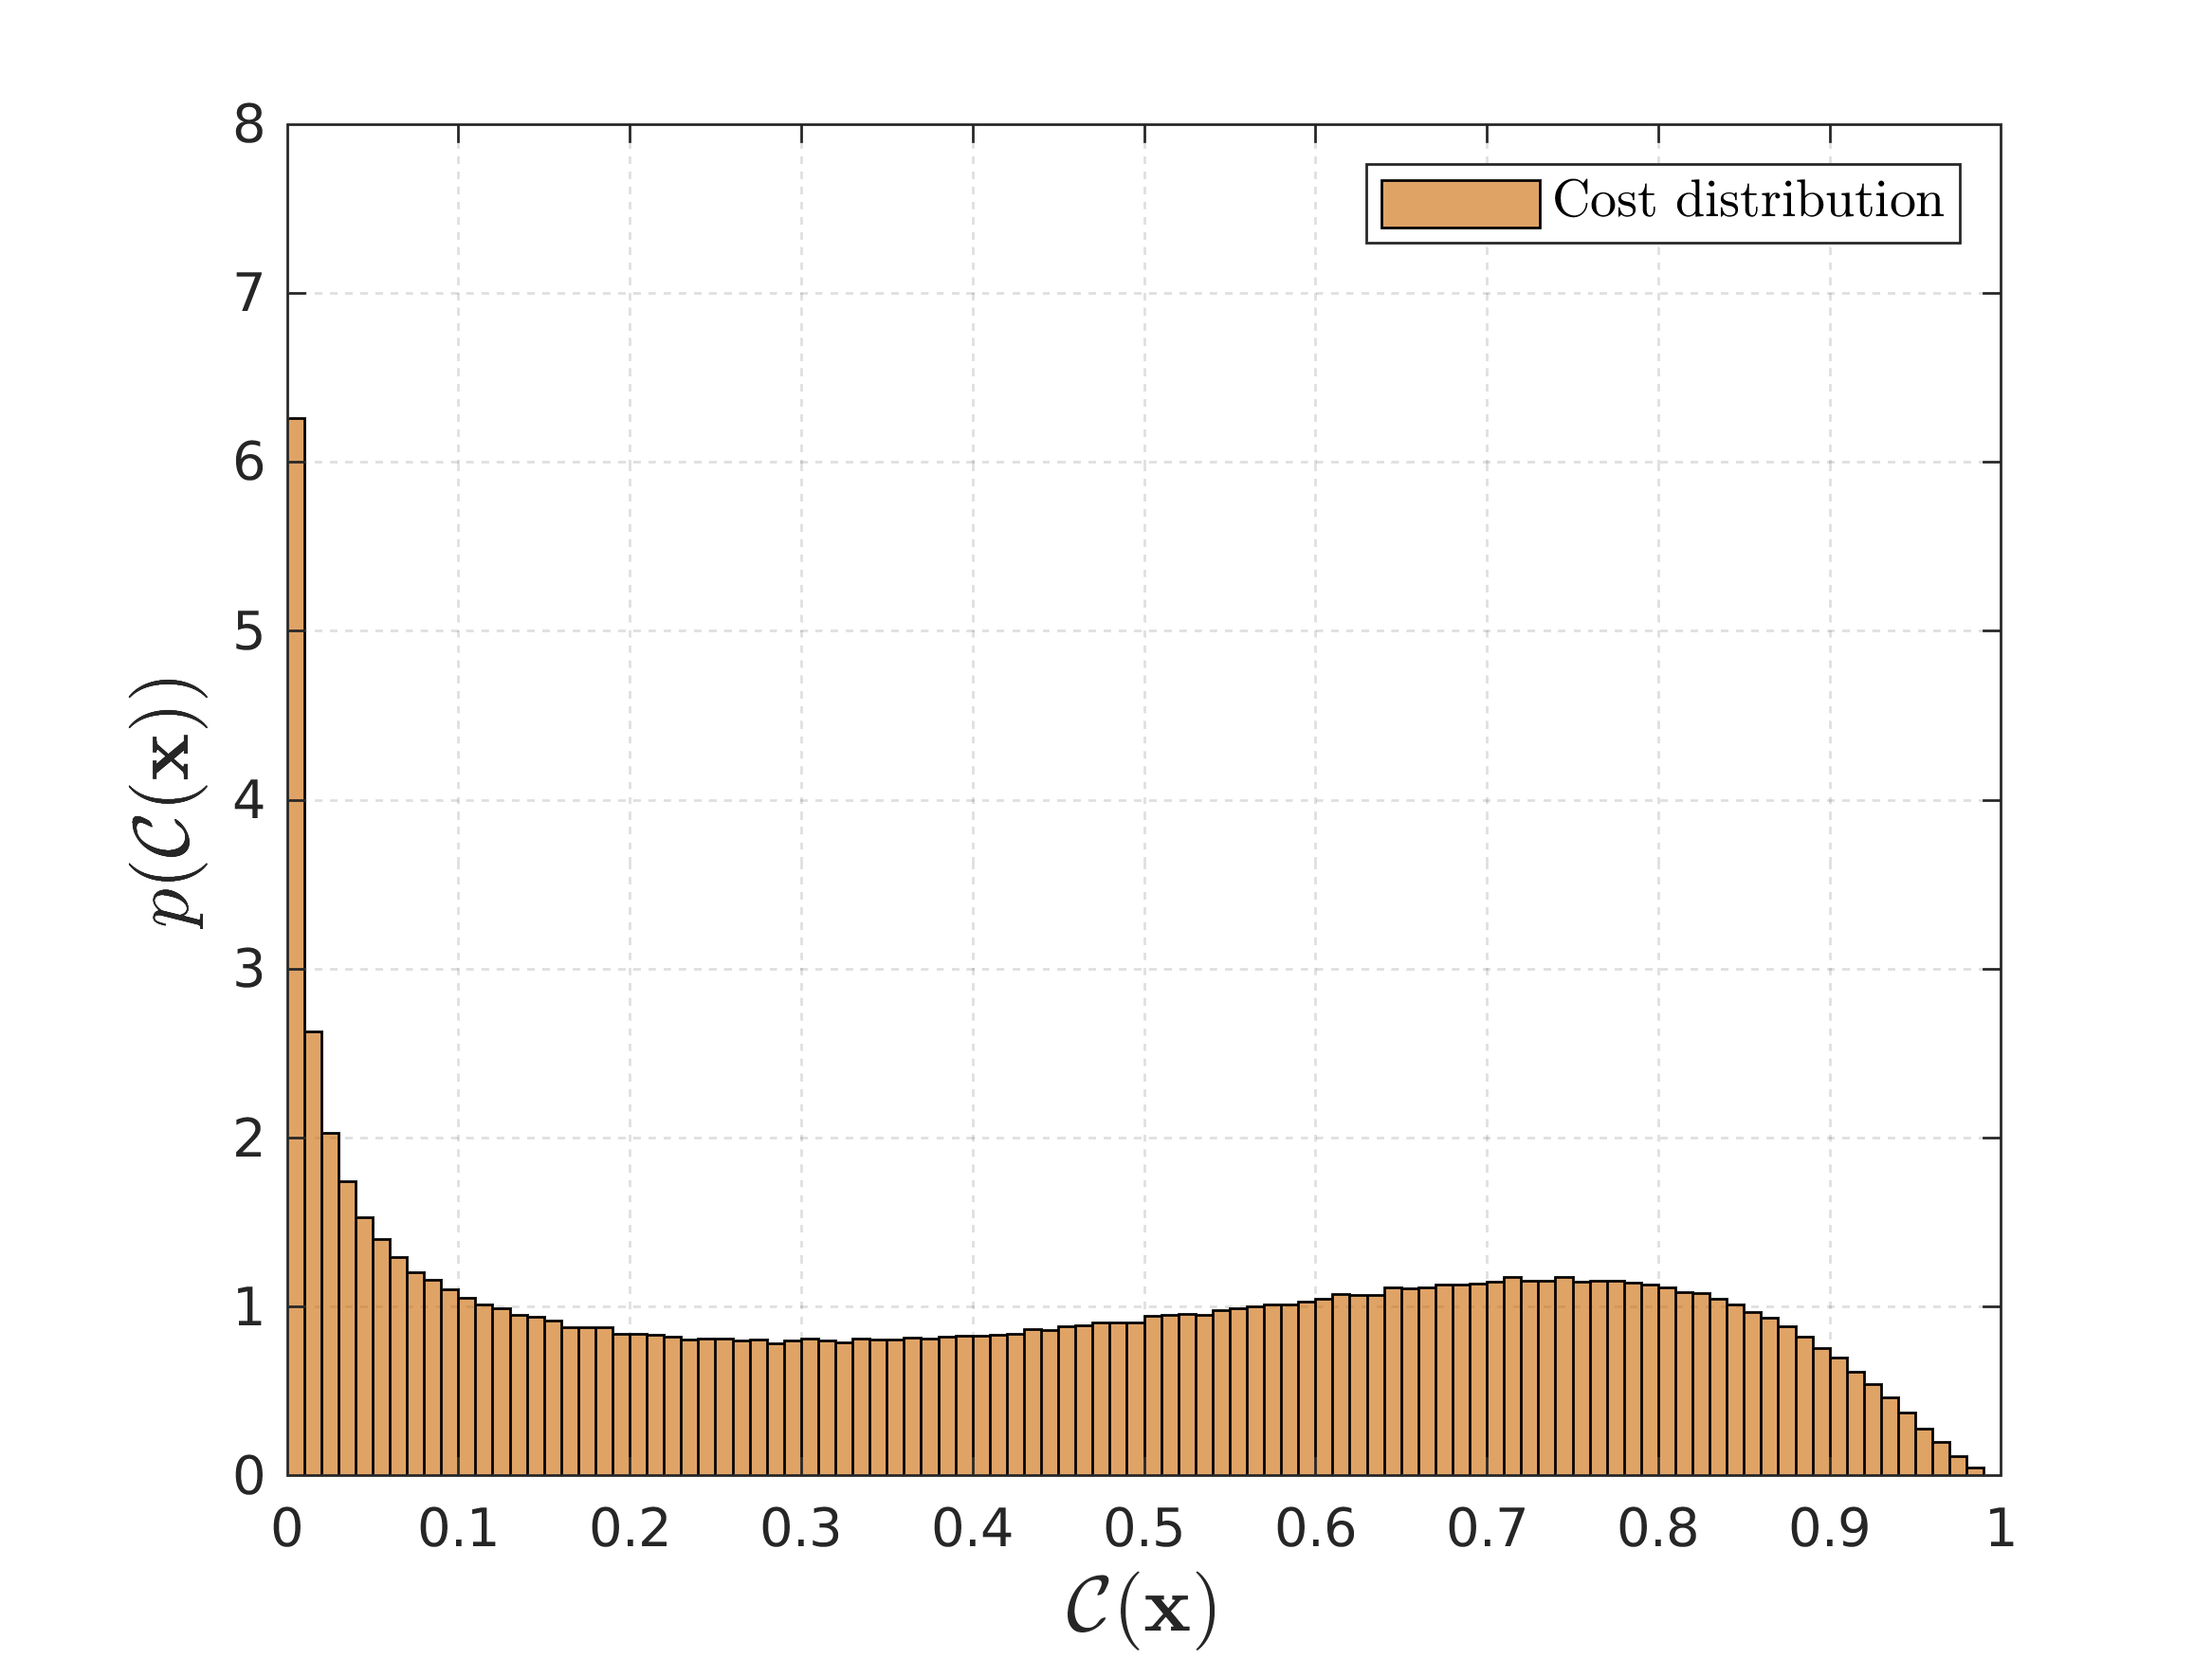
\includegraphics[height=0.22\textheight,width=0.95\textwidth]{Chapter3/Figures/trans_cost_hist_4.png} 
    \caption{Distribution over costs after 9 transitions} 
    \label{Fig:Re-hist-cost-4} 
  \end{subfigure} 
\caption[Evolution of state and cost distributions]{The evolution of state and cost distributions with increasing numbers of steps through the transition function.}
\label{Fig:Re-evolution-of-state-and-cost} 
\end{figure}

\subsection{A Decomposition of Cost Function Uncertainty}
A toy data set with target noise variance 0.0625 is used to illustrate the Monte Carlo scheme for estimating the aleatoric and epistemic uncertainties present in the cost $\mathbb{C}(\mathbf{x})$ under policy $\pi$. Similar to the previous experiment, a 1-dimensional transition function is used and an explicit policy is not defined. This is viewed as if there is only one action available for selection and the agent selects that action at each opportunity which allows the system dynamics to evolve freely over time. In this experiment, the agent begins by observing 4 transition data points. It then progressively observes more data a single point at a time up to a total of 50 data points. At each observation, the trigonometric basis function model is used to form a belief over the transition dynamics of the environment. Fig. \ref{Fig:Re-pred-4-points}-\ref{Fig:Re-pred-50-points} shows the predictive distribution over the transition data and 4 functions sampled from the posterior distribution over the parameters after 4, 25 and 50 observations, respectively. For this, the lengthscale of the spectral points is purposely set to a large value to over fit the data as can be seen in Fig. \ref{Fig:Re-pred-4-points}. This is done for two reasons: to artificially induce more epistemic uncertainty into the model and to be more representative of a higher dimensional space where the observation of a single data point provides the model with more information than in the 1-dimensional case. The figures show that as more data is observed, the model becomes increasingly confident about the parameters. This can be seen in the functions drawn from the posterior distribution over the model parameters which increasingly resemble the predictive mean as confidence grows. 

Each time a new data point is observed, Monte Carlo trajectory roll-outs are performed through the model using the procedure described in Sec. \ref{S:monte-carlo-estimate}, the cost is calculated for a target of $x=0$ and the uncertainty in the cost is decomposed into its aleatoric and epistemic components using Eq. \ref{S:monte-carlo-estimate}. The Monte Carlo roll-outs are performed for $(M=100,\: N=100,\: T=100)$ and transition noise of variance 0.09. It is important to note that the sources of uncertainty arise within the model and the transitions through the model but they are measured here with respect to the cost. 

Fig. \ref{Fig:Re-reduction-in-epsitemic-with-more-data} shows the uncertainty breakdown as a function of number of data points. As the number of data points increases the model becomes more confident about the parameters and the epistemic uncertainty decreases. With the reduction in epistemic uncertainty, the total uncertainty also reduces and the gap between the aleatoric and total uncertainty decreases. This is because each time the roll-outs are performed, they are done so under the same policy. Should the policy be different after each new observation (as is typically the case after observing new data) the uncertainties would be different under each policy as will be demonstrated for the PILCO experiments. Finally, one might expect the epistemic uncertainty to decrease monotonically as more data is observed and roll-outs are performed under the same policy, but the reduction appears noisy. This could be a consequence of the Monte Carlo approach and should reduce with a larger number of roll-outs.
 
\begin{figure}[htbp]    
  \begin{subfigure}[b]{0.95\linewidth}
    \centering
    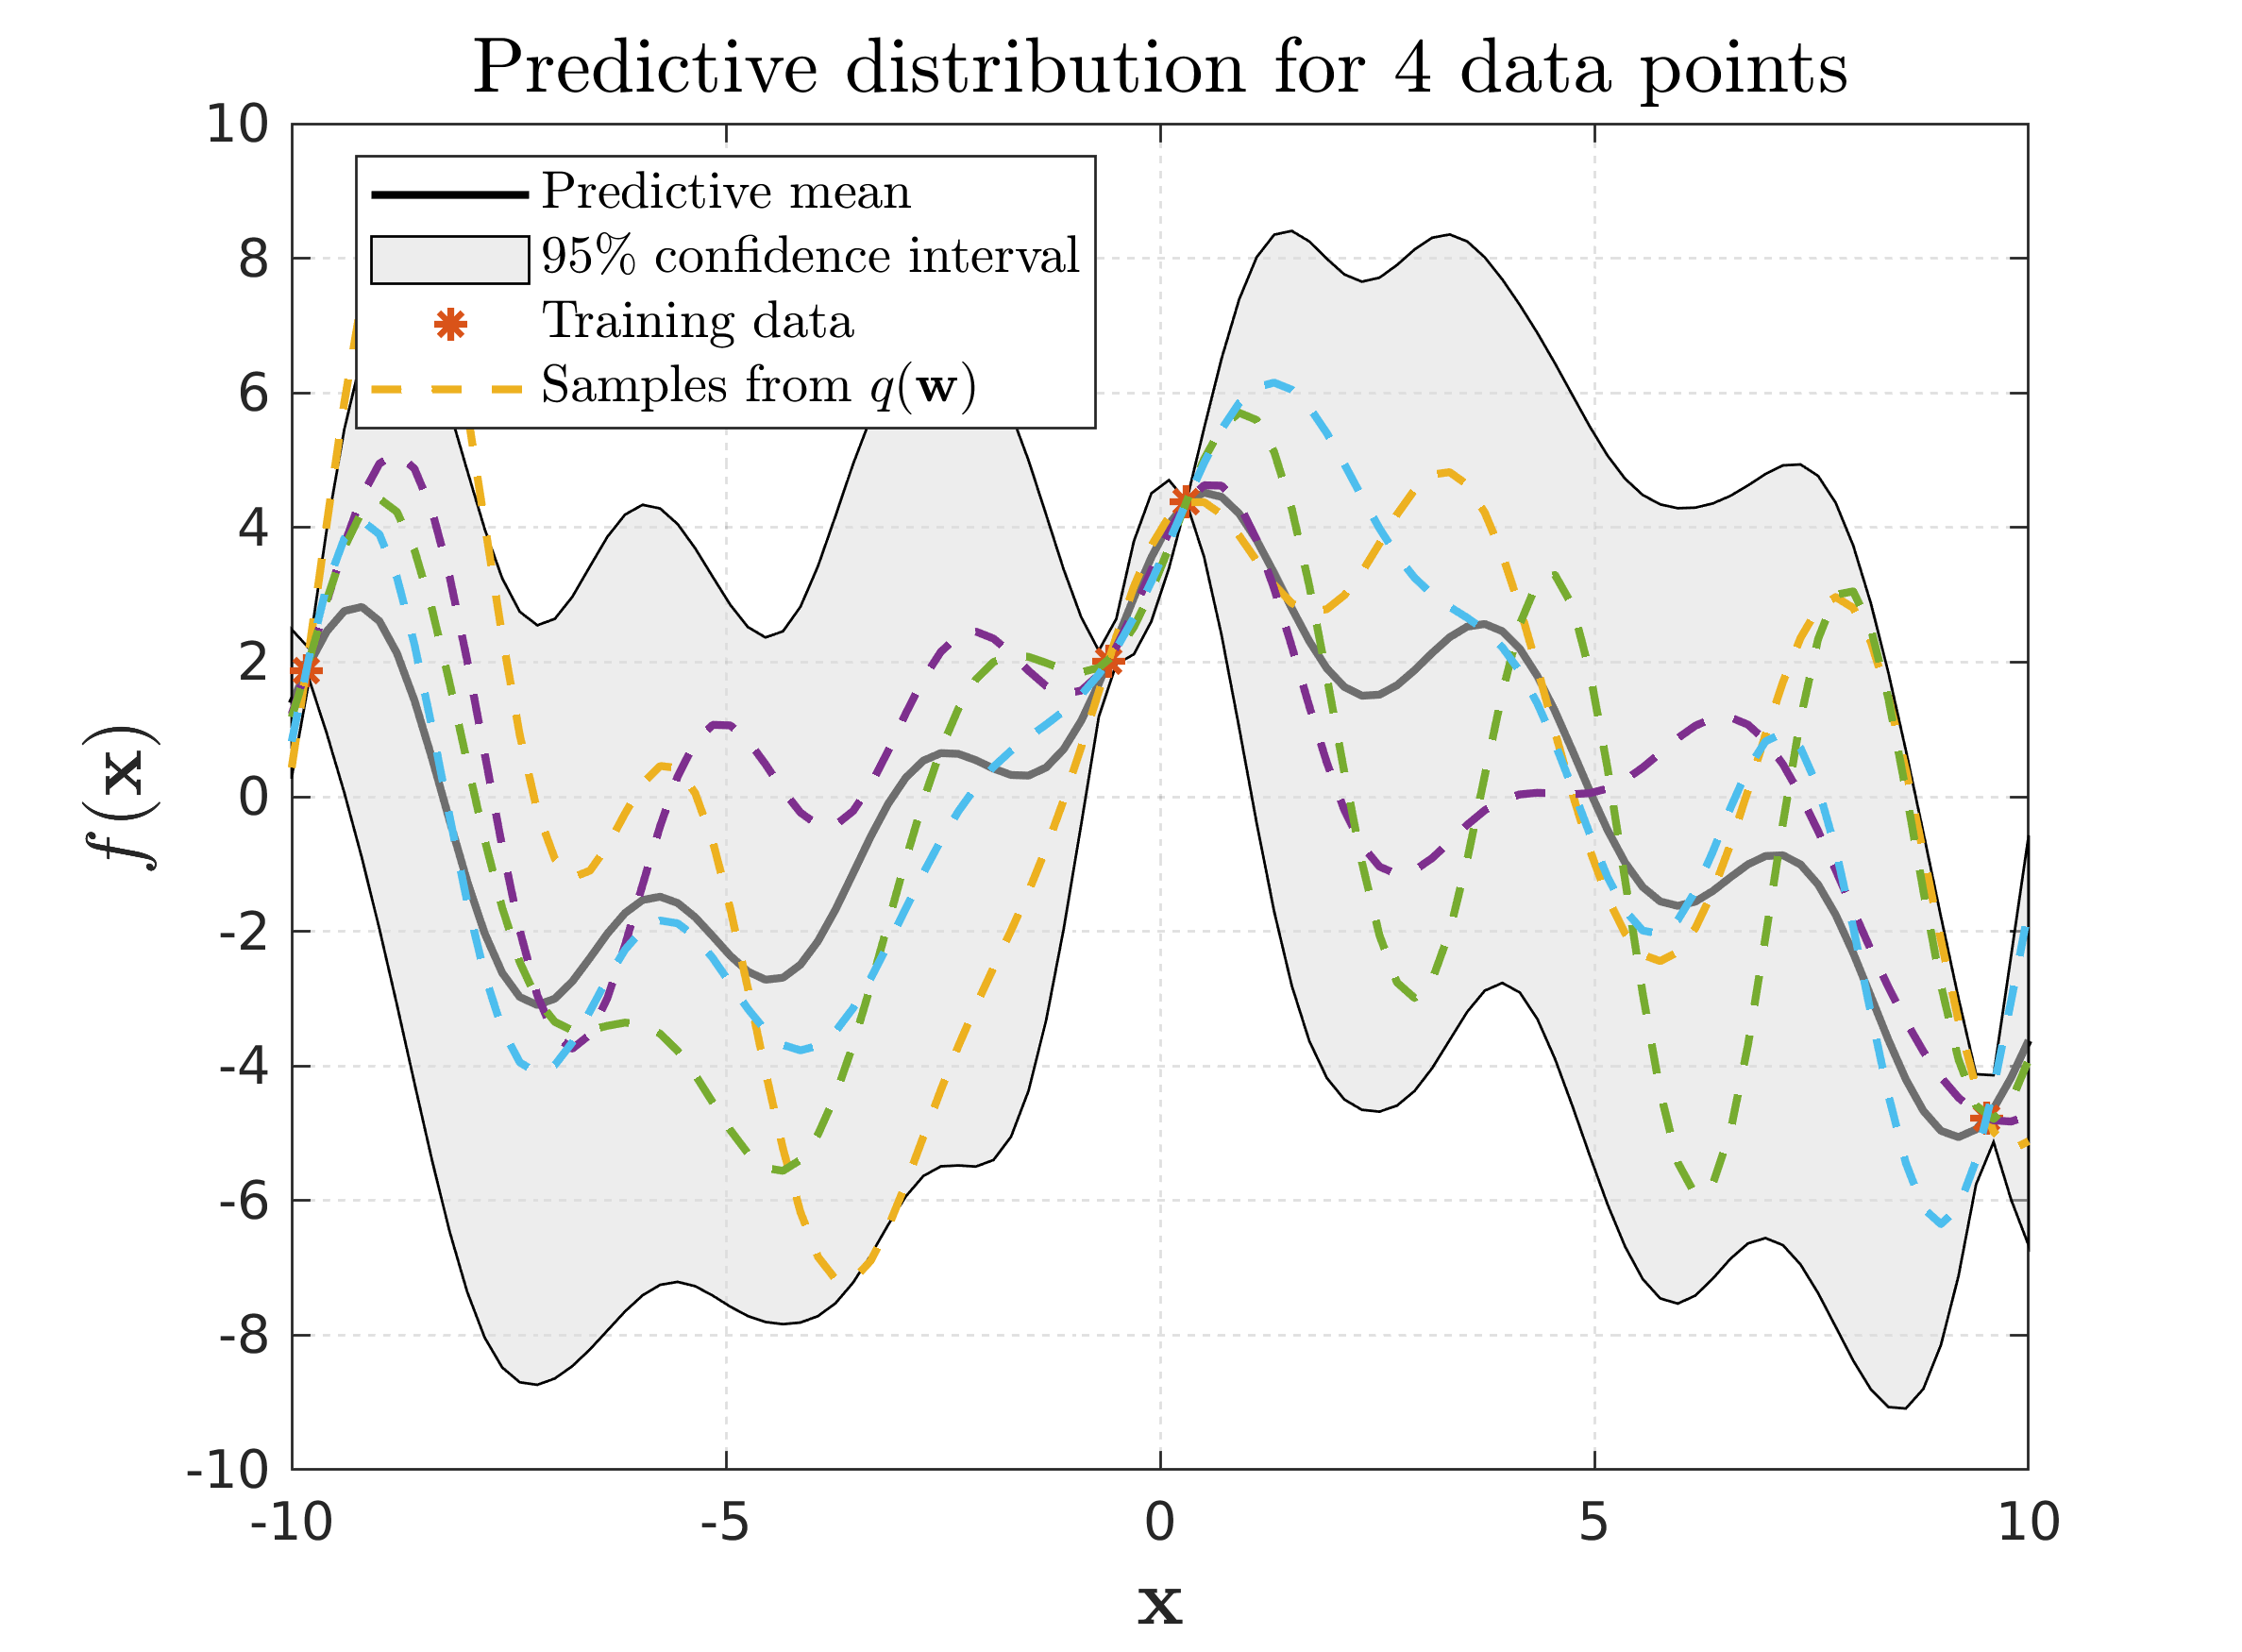
\includegraphics[trim={0 0.18cm 0 0.70cm},clip,height=0.27\textheight,width=0.75\textwidth]{Chapter3/Figures/func_uncertainty_1.png} 
    \caption{Predictive distribution for 4 data points} 
    \label{Fig:Re-pred-4-points} 
  \end{subfigure}

  \begin{subfigure}[b]{0.95\linewidth}
    \centering
    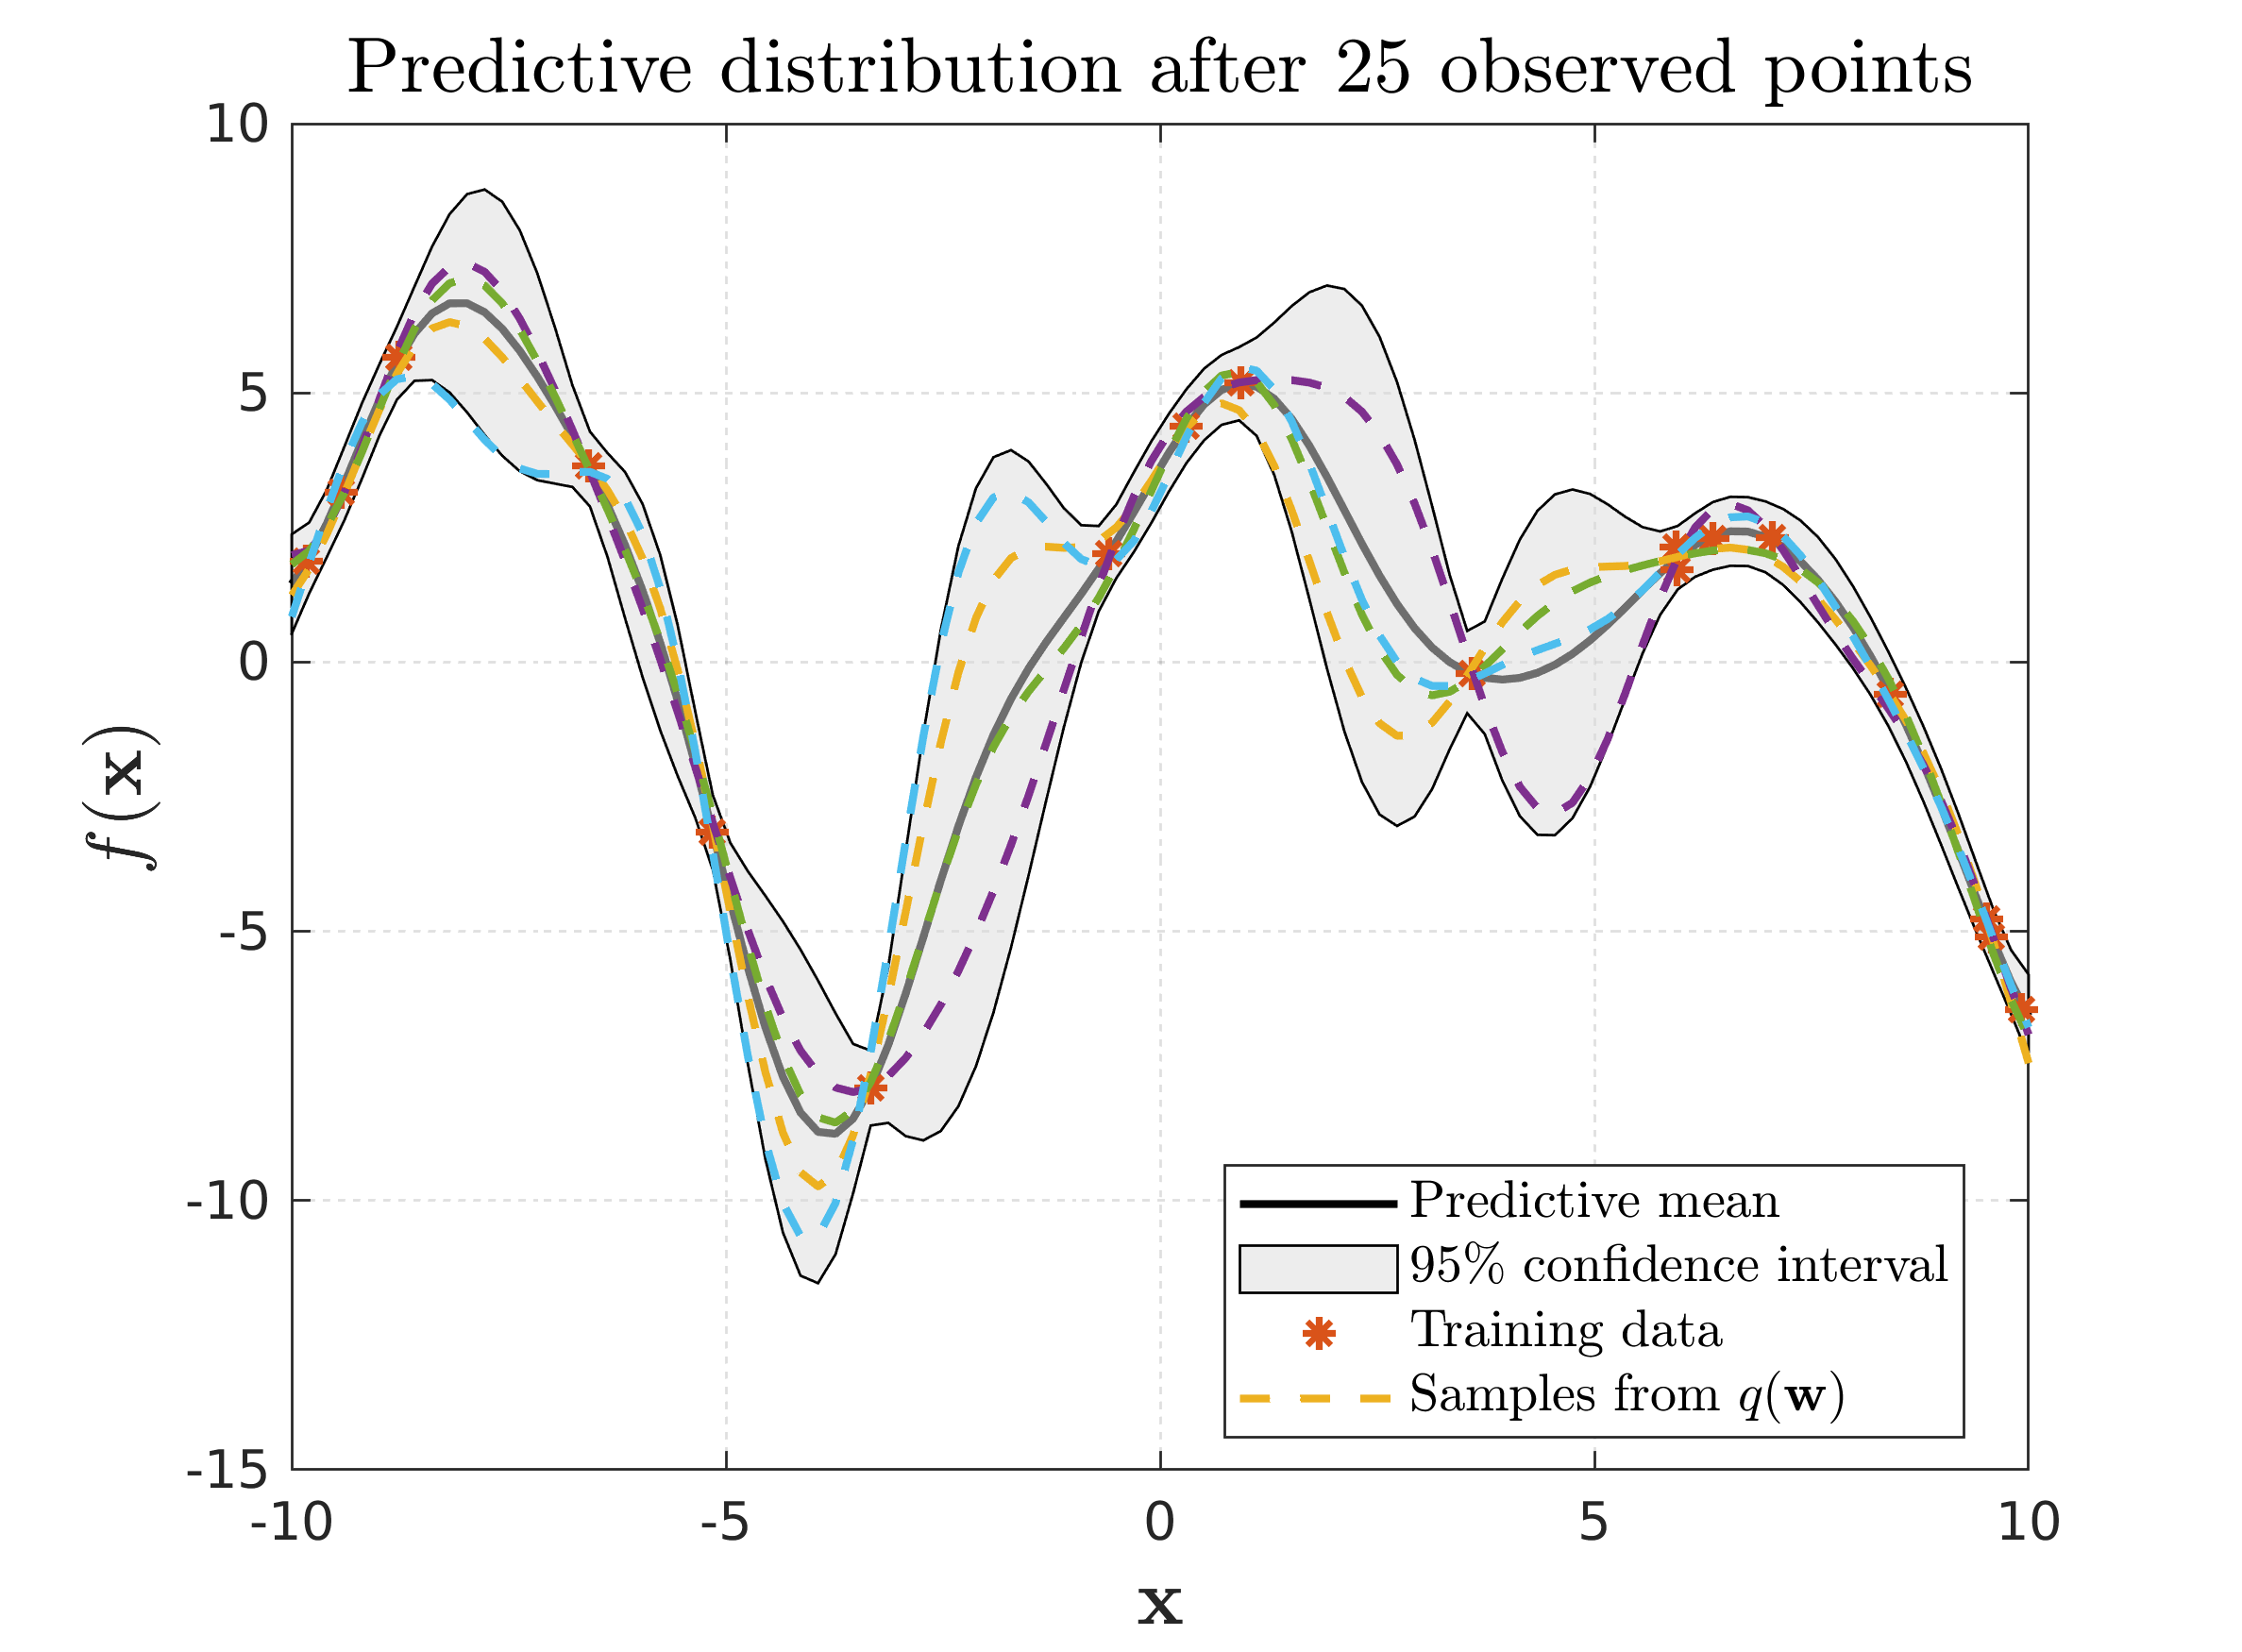
\includegraphics[trim={0 0.18cm 0 0.70cm},clip,height=0.27\textheight,width=0.75\textwidth]{Chapter3/Figures/func_uncertainty_2.png} 
    \caption{Predictive distribution after 25 data points} 
    \label{Fig:Re-pred-25-points}
  \end{subfigure}
  
  \begin{subfigure}[b]{0.95\linewidth}
    \centering
    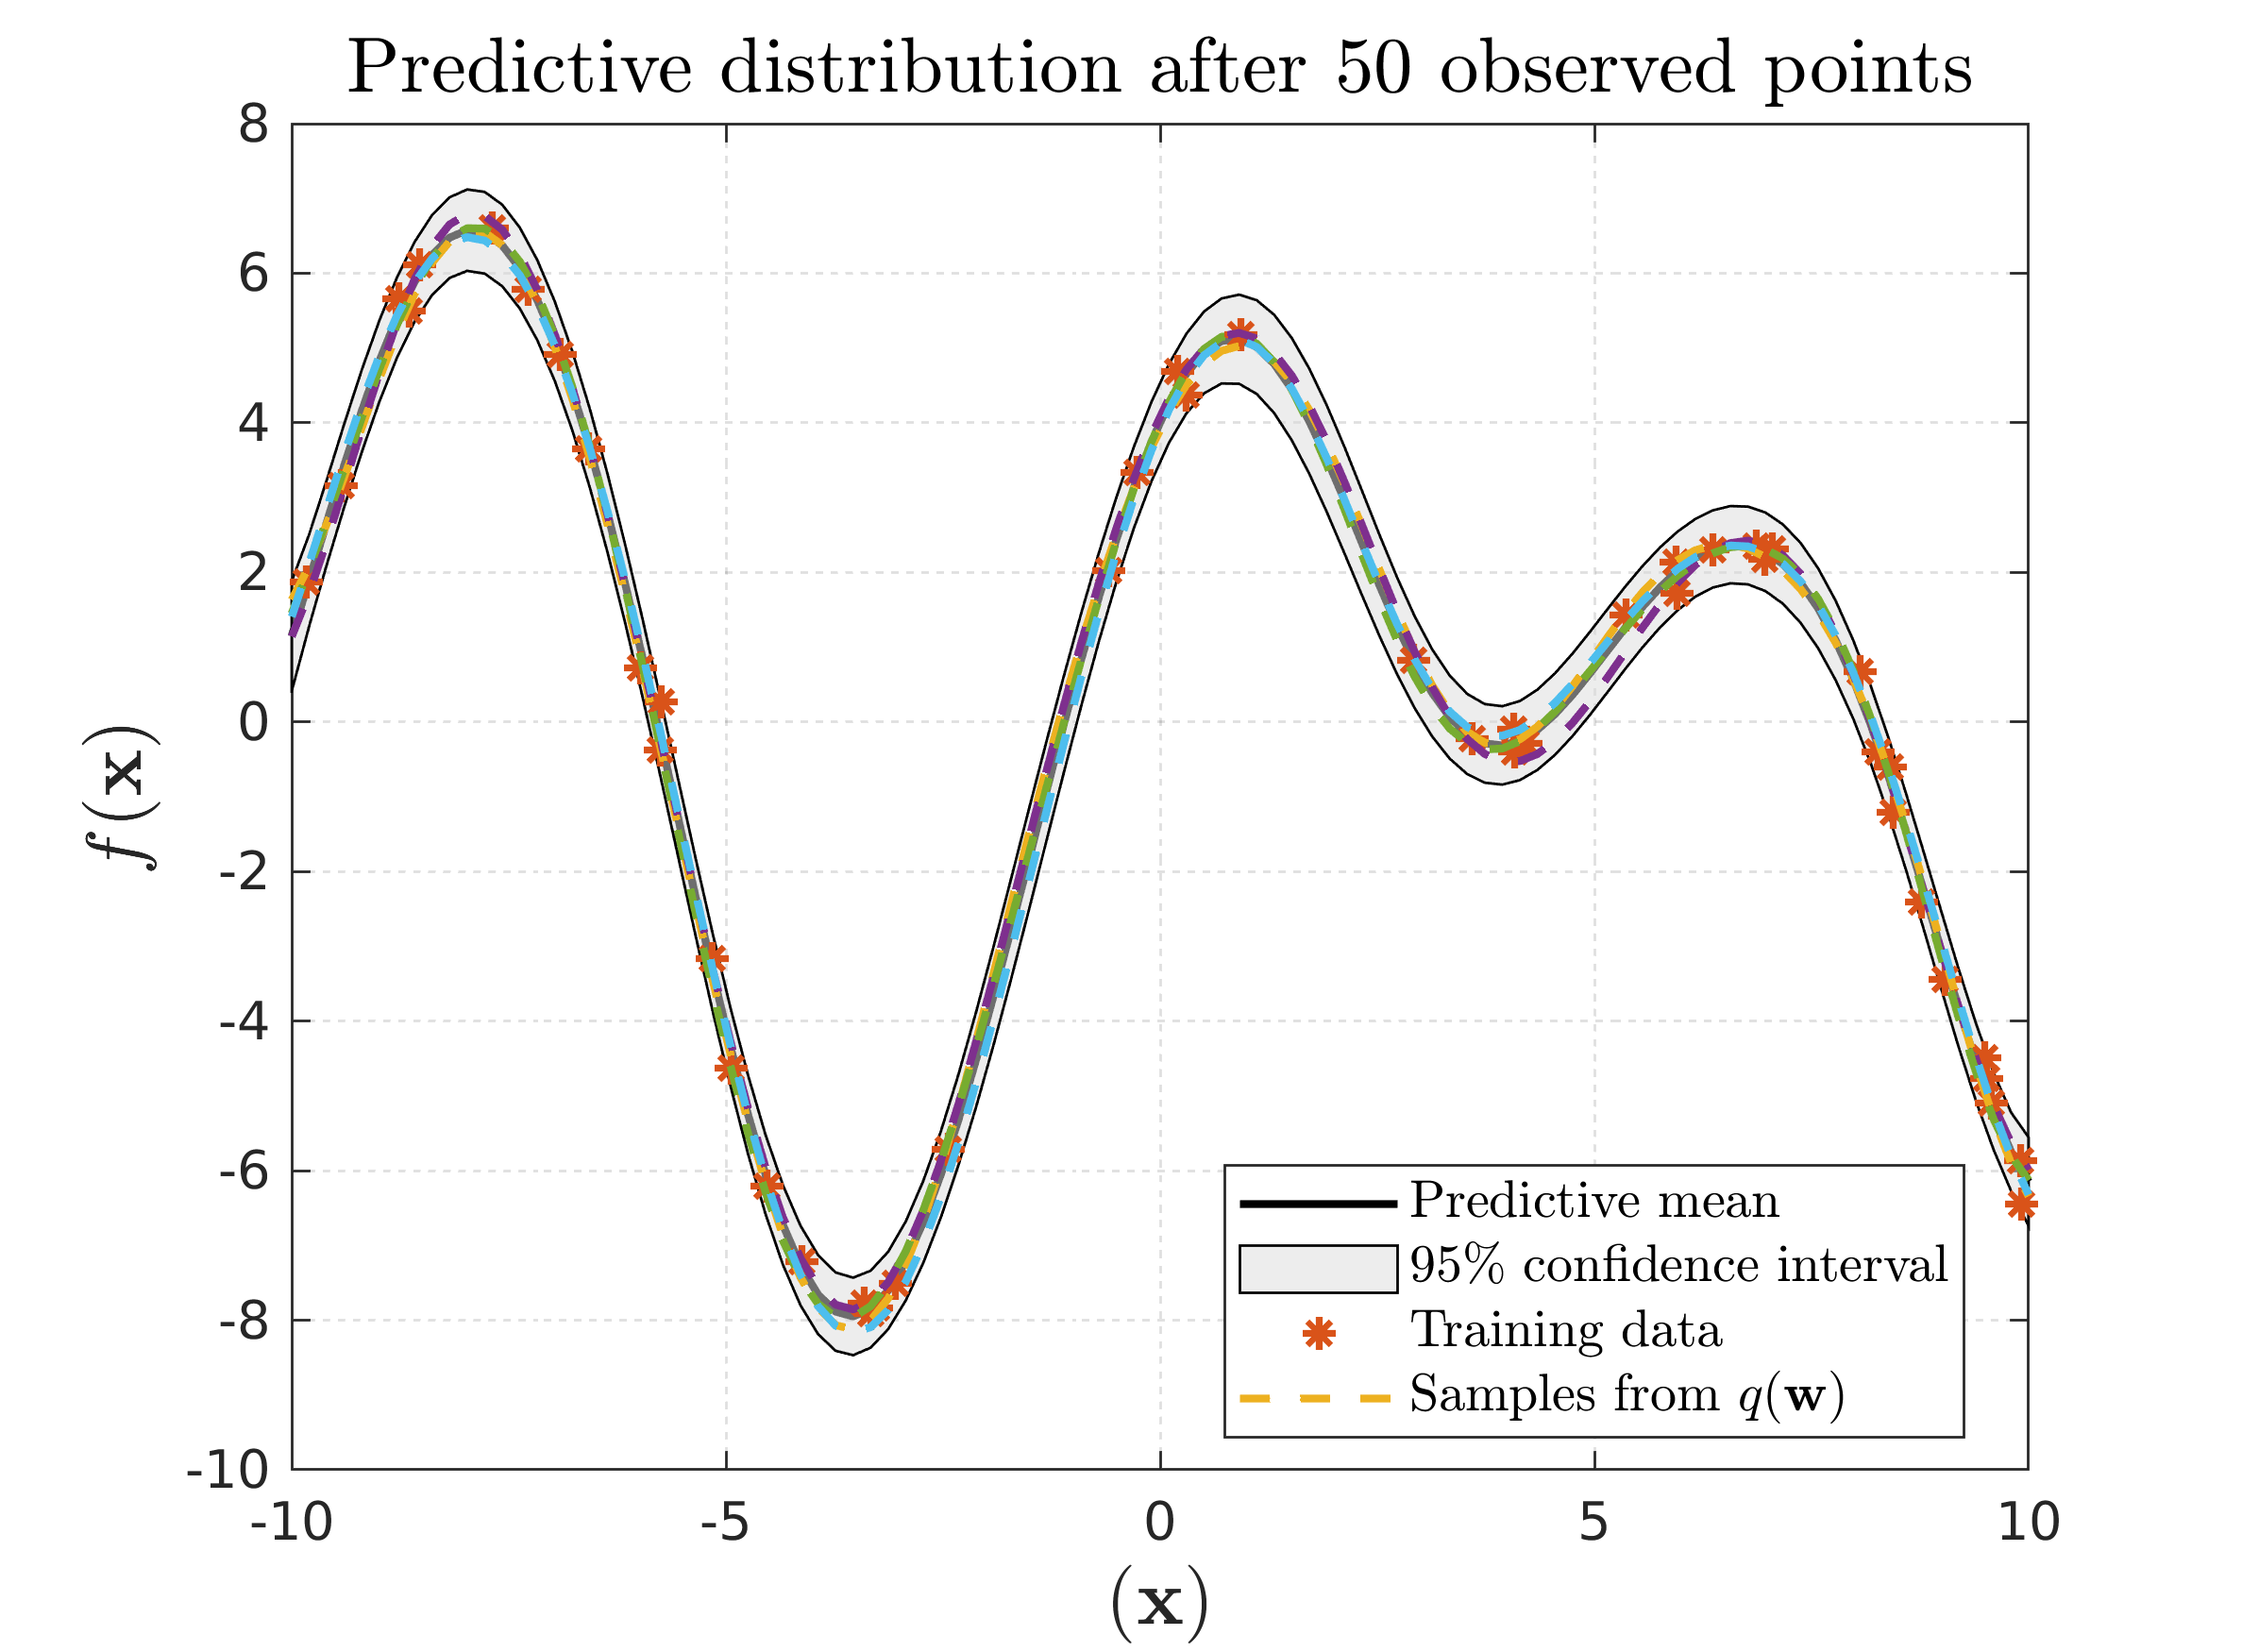
\includegraphics[trim={0 0.1cm 0 0.70cm},clip,height=0.27\textheight,width=0.75\textwidth]{Chapter3/Figures/func_uncertainty_3.png} 
    \caption{Predictive distribution after 50 data points} 
    \label{Fig:Re-pred-50-points}
  \end{subfigure}
 
\caption[Reduction in epistemic uncertainty with added data]{: Fig \ref{Fig:Re-pred-4-points} - \ref{Fig:Re-pred-50-points} show the predictive distribution over the data and samples from the posterior after 4, 25 and 50 observed data points. The lengthscale of the spectral points is purposely set to a high value to over fit the data and imitate high dimensional space. As more data is observed the model becomes increasingly confident about the parameter values and as a consequence the posterior distribution narrows.}
\label{Fig:Re-predictive-fit-to-varying-number-of-datapoints} 
\end{figure}

\begin{figure}[htbp]
\centering    
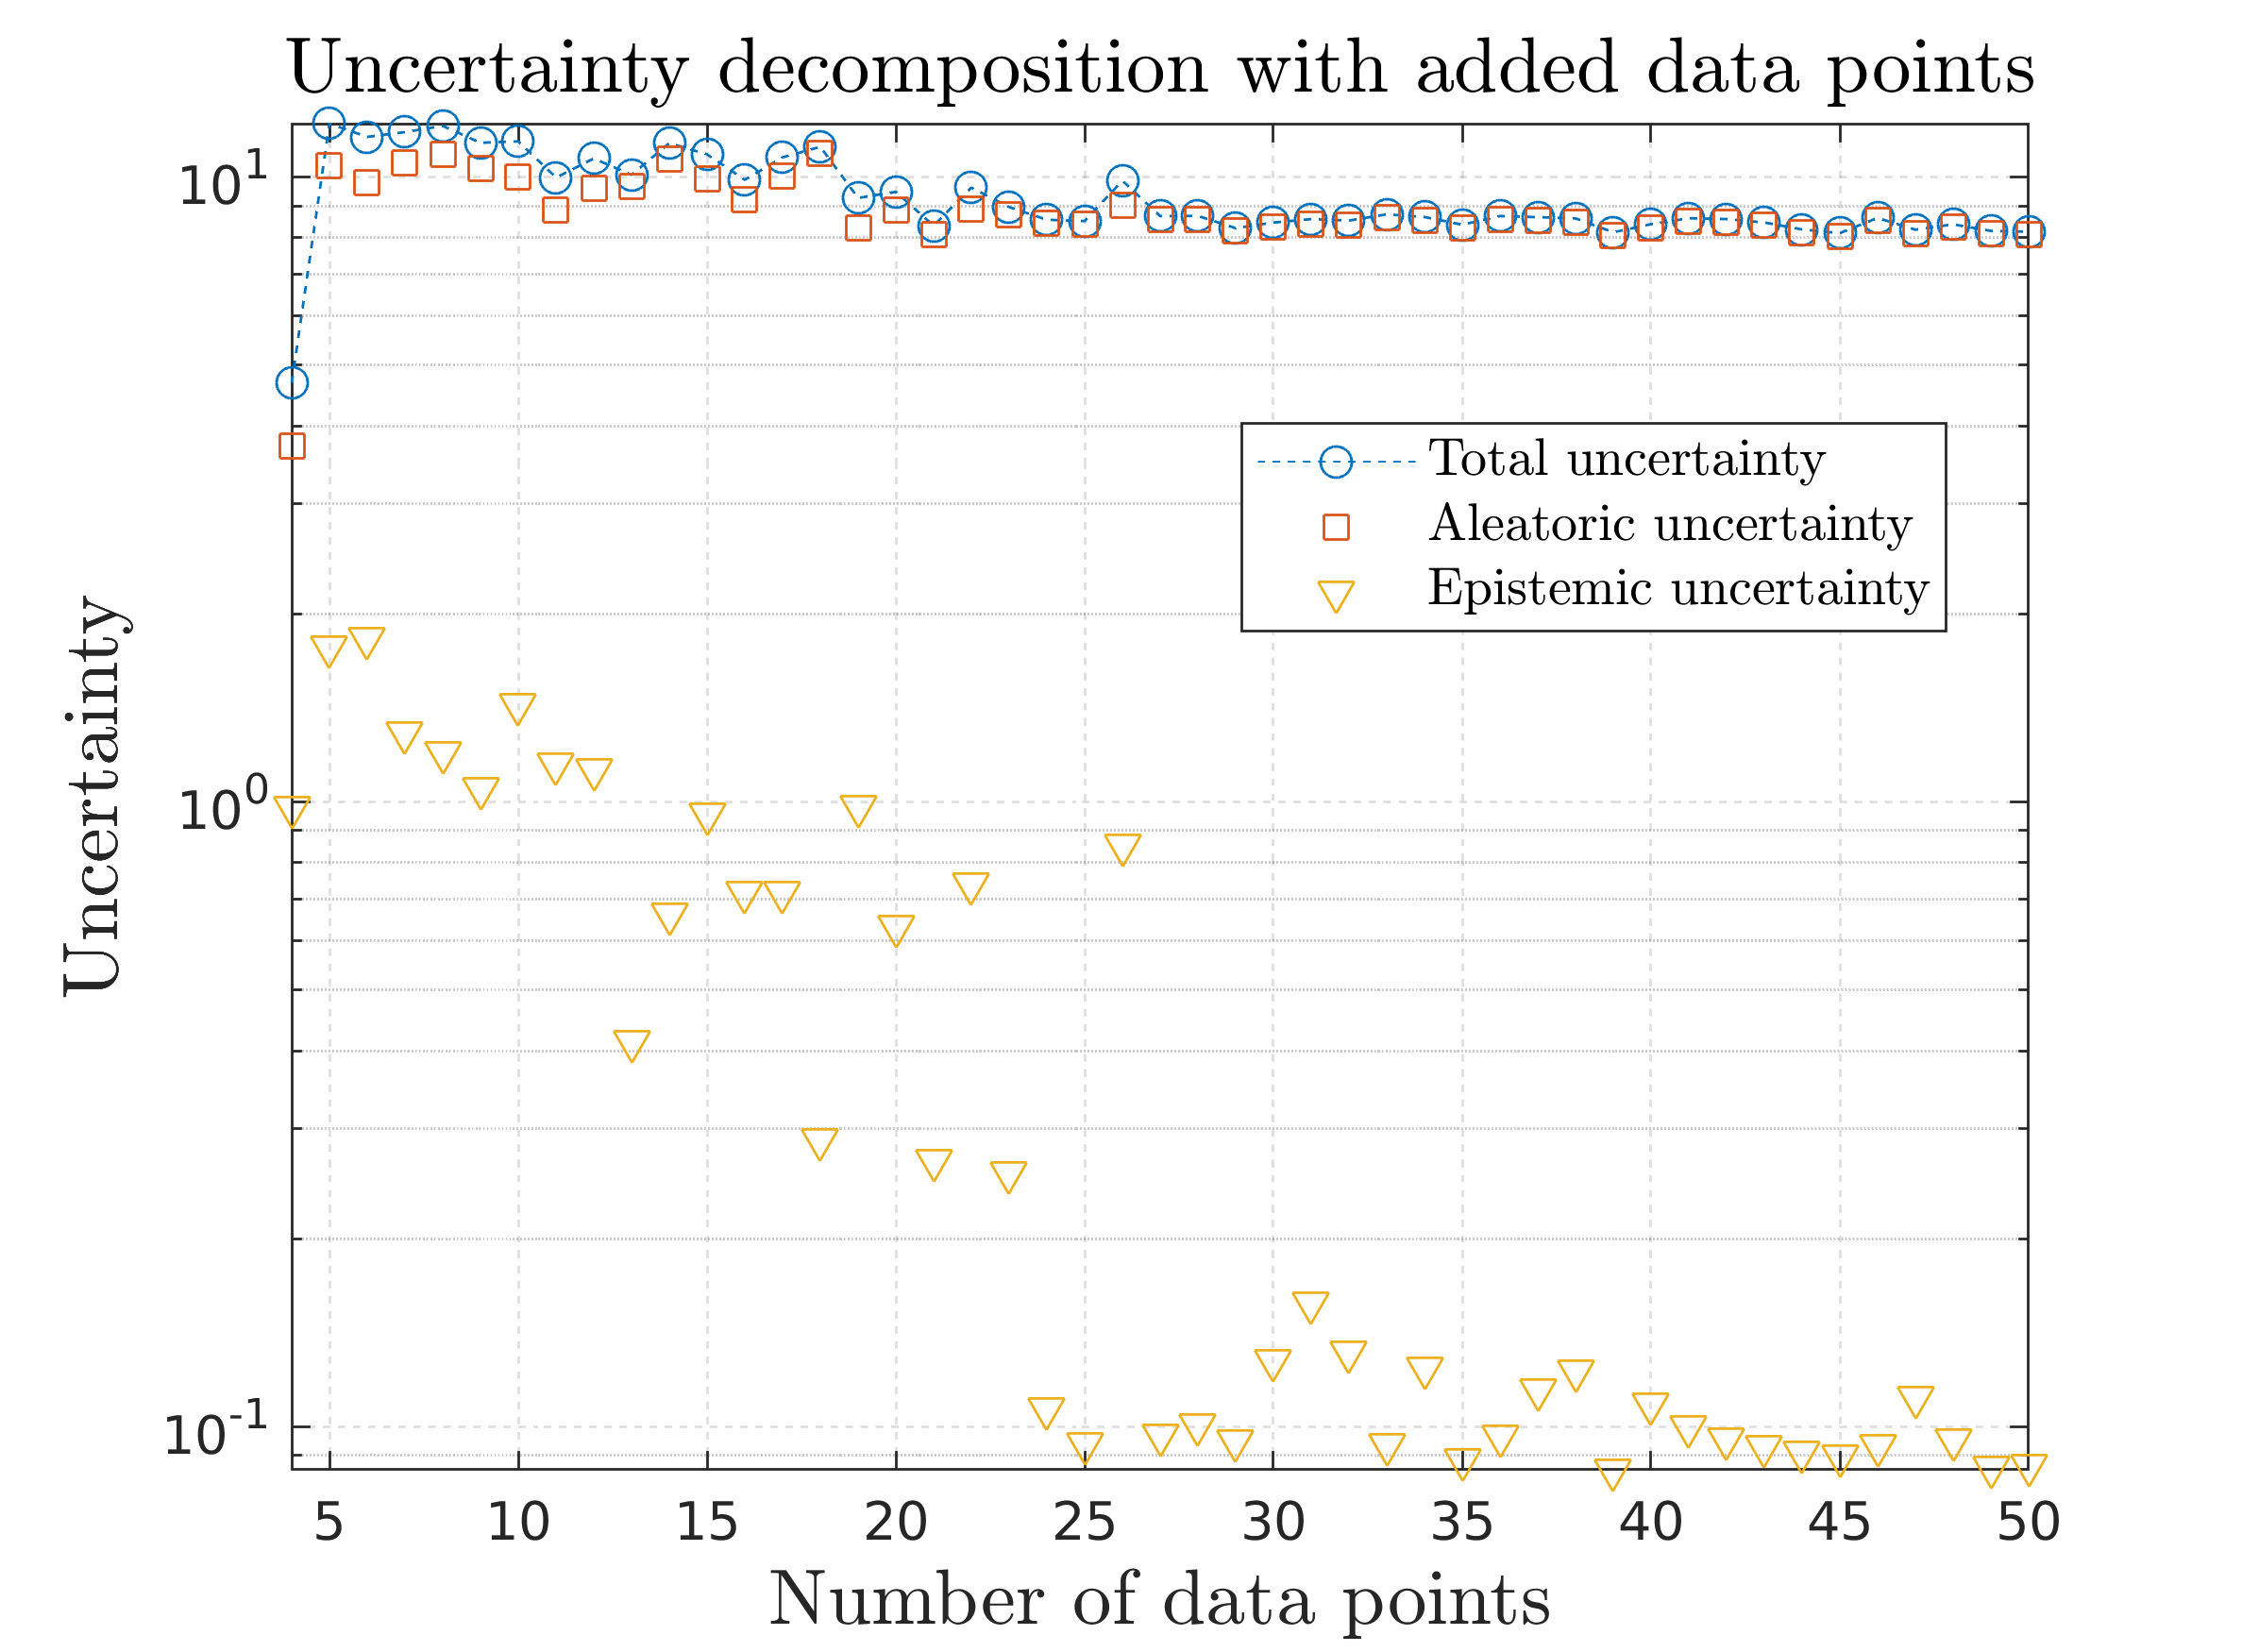
\includegraphics[width=1\textwidth]{Chapter3/Figures/func_uncertainty_4.png}
\caption[Uncertainty decomposition showing reduction in epistemic uncertainty with increasing number of data points]{Relating to Fig. \ref{Fig:Re-predictive-fit-to-varying-number-of-datapoints}. Trajectory roll-outs are performed through the transition function each time a new data point is observed (from 4 to 50). For each roll-out the uncertainty in the cost is decomposed. As more data is observed the model becomes increasingly confident about its parameters and consequently the epistemic uncertainty reduces due to contraction of the posterior distribution.}
\label{Fig:Re-reduction-in-epsitemic-with-more-data}
\end{figure}


\subsection{The Effect of Cost Function Uncertainty on Learning}
\label{S:Re-PILCO-envs}
In this section, I present the Monte Carlo uncertainty analyses for the 3 PILCO environments introduced in section \ref{S:PILCO-environments}. The procedure to produce the results is as follows. After each PILCO episode, I train the trigonometric basis function model (see section \ref{S:approximating-pilcos-gp}) on all the observed data up to the end of that episode. The inputs are the state-action tuples and the targets are the state differences. Conditionally independent models are trained for each target dimension. In all cases, I use 500 basis functions. The Monte Carlo trajectory roll-outs are performed according to algorithm \ref{GSMCUE:algorithm} under policy $\pi$ for $(M=100,\:N=100,\:T=T_{E})$, where $T_{E}$ and the transition noise $\boldgreek{\varepsilon}_{E}$ are environment specific. I then decompose the total uncertainty into uncertainties representing total aleatoric and total epistemic uncertainty in the cost $\mathbb{C}(\mathbf{x})$ under policy $\pi$ for an entire episode, following the procedure detailed in section  

For each environment, I present figures that show the following:
\begin{itemize}
    \item A random sample of the Monte Carlo trajectory roll-outs for each of the state variables that describe the environment. For each figure the left axis represents the state variable and corresponds to trends for the Monte Carlo trajectories, the actual trajectory recorded during that episode, the target of the state variable and PILCO's prediction of the state evolution before the episode. The right axis shows the percentage of Monte Carlo trajectories that fall within the 2 standard deviation error bars of PILCO's prediction for that time step;
    \item The average cost and cost uncertainty decomposition under policy $\pi$ for each each episode. The average cost per episode is shown of the left axis which is indicative of learning. High cost indicates that the agent is not achieving the objective, low cost indicates the objective is being achieved and a decreasing average cost indicates the agent is learning. The right axis shows total cost uncertainty and its decomposition into aleatoric epistemic cost uncertainty;
    \item The average cost and the ratio of epistemic cost uncertainty to total cost uncertainty under policy $\pi$ for each each episode. The left axis shows the average cost and the right axis the ratio of epistemic cost uncertainty to total cost uncertainty.
\end{itemize}

\subsubsection{Cart-pole}
Figures \ref{Fig:Re-cp-MC-roll-outs-1} and \ref{Fig:Re-cp-MC-roll-outs-2} show a random sample of the Monte Carlo trajectory roll-outs for the state variables of the cart-pole environment: cart position $x$ and cart velocity $\dot{x}$ (fig. \ref{Fig:Re-cp-MC-roll-outs-1}), and pendulum angular velocity $\dot \theta$ and pendulum angle $\theta$ (fig. \ref{Fig:Re-cp-MC-roll-outs-2}). In both figures, the left vertical axis represents the state variable and corresponds to the trends for the Monte Carlo trajectories, the actual trajectory recorded during that episode, the target of the state variable, and PILCO's prediction of the state evolution before the episode. The right axis shows the percentage of Monte Carlo trajectories that fall within the 2 standard deviation error bars of PILCO's prediction for that time step. The trajectories shown are from episode 15, when PILCO has achieved the environment objective, and so represent trajectories under a mature policy $\pi$. For the cart-pole environment, a high agreement (greater than $80\%$) is noted between the Monte Carlo trajectories and PILCO's prediction of the state evolution.

Fig. \ref{Fig:Re-cp-full-uncertainty} shows the average cost per episode and cost uncertainty decomposition under policy $\pi$ over the course of learning. Panel \ref{Fig:Re-cp-uncertainty} shows the full uncertainty decomposition and panel \ref{Fig:Re-cp-uncertainty-norm} shows the ratio of epistemic to total uncertainty. The average cost per episode, shown on the left vertical axes, is indicative of success in learning. High cost indicates that the agent is not achieving the objective, low cost indicates the objective is being achieved and a decreasing average cost indicates that the agent is learning. The right axis shows total cost uncertainty and its decomposition into aleatoric and epistemic cost uncertainty. 

The average cost per episode exhibits a sharp decline early in the learning process (this can be seen in both panels of the figure) and by the third episode PILCO has solved the environment. This is the simplest of the environments tested and because PILCO solves it early in the learning process, we cannot gain much insight into how the cost uncertainty varies. In episode zero (not shown in the figures), PILCO performs a series of roll-outs under a random policy to generate initial state observations. It is likely, particularly in the case where the state-space is well explored during the random roll-out, that these data are enough for the algorithm to find a low cost policy that solves the environment early in the learning process. Consequently, for episodes 1-3 the selected policy contains little epistemic cost uncertainty because the model is already confident about its beliefs and a successful low cost policy exists. 

Interestingly, for episodes 7 and 8, PILCO selects policies with high epistemic uncertainty in the cost and does so after it has already solved the environment. This could be due to PILCO's unintentional exploration mechanism where it favours uncertain states. After this (Fig. \ref{Fig:Re-cp-uncertainty} episodes 9-15), the total and aleatoric uncertainties settle and the epistemic reduces, indicating that the model is now confident in its model of parts of the state-space associated with low cost.

% \begin{table}
% \caption{Even better looking table using booktabs}
% \centering
% \label{table:good_table}
% \begin{tabular}{l c c c c c c}
% \toprule
% \multirow{2}{*}{State variable} & \multicolumn{2}{c}{Cart-pole} & \multicolumn{2}{c}{Pendubot}  &
% \multicolumn{2}{c}{Cart-double-pendulum}  \\ 
% \cmidrule{2-7}
%   & Start & Target & Start & Target & Start & Target \\ 
% \midrule
% Cart position $x_1$ & & & & & & \\

% Cart velocity $\dot x_1$ & & & & & & \\

% Angle 2 $\theta_2$ & & & & & & \\

% Angle 3 $\theta_3$ & & & & & &\\

% Angular velocity 2 $\dot \theta_2$ & 13.47 & 0.09 & 10.55 & 0.05 & &\\

% Angular velocity 3 $\dot \theta_3$ & 11.88 & 0.05 & 13.11 & 0.04& &\\ 
% \bottomrule
% \end{tabular}
% \end{table}

\begin{figure}[htbp]    
   \begin{subfigure}[b]{1\linewidth}
    \centering
    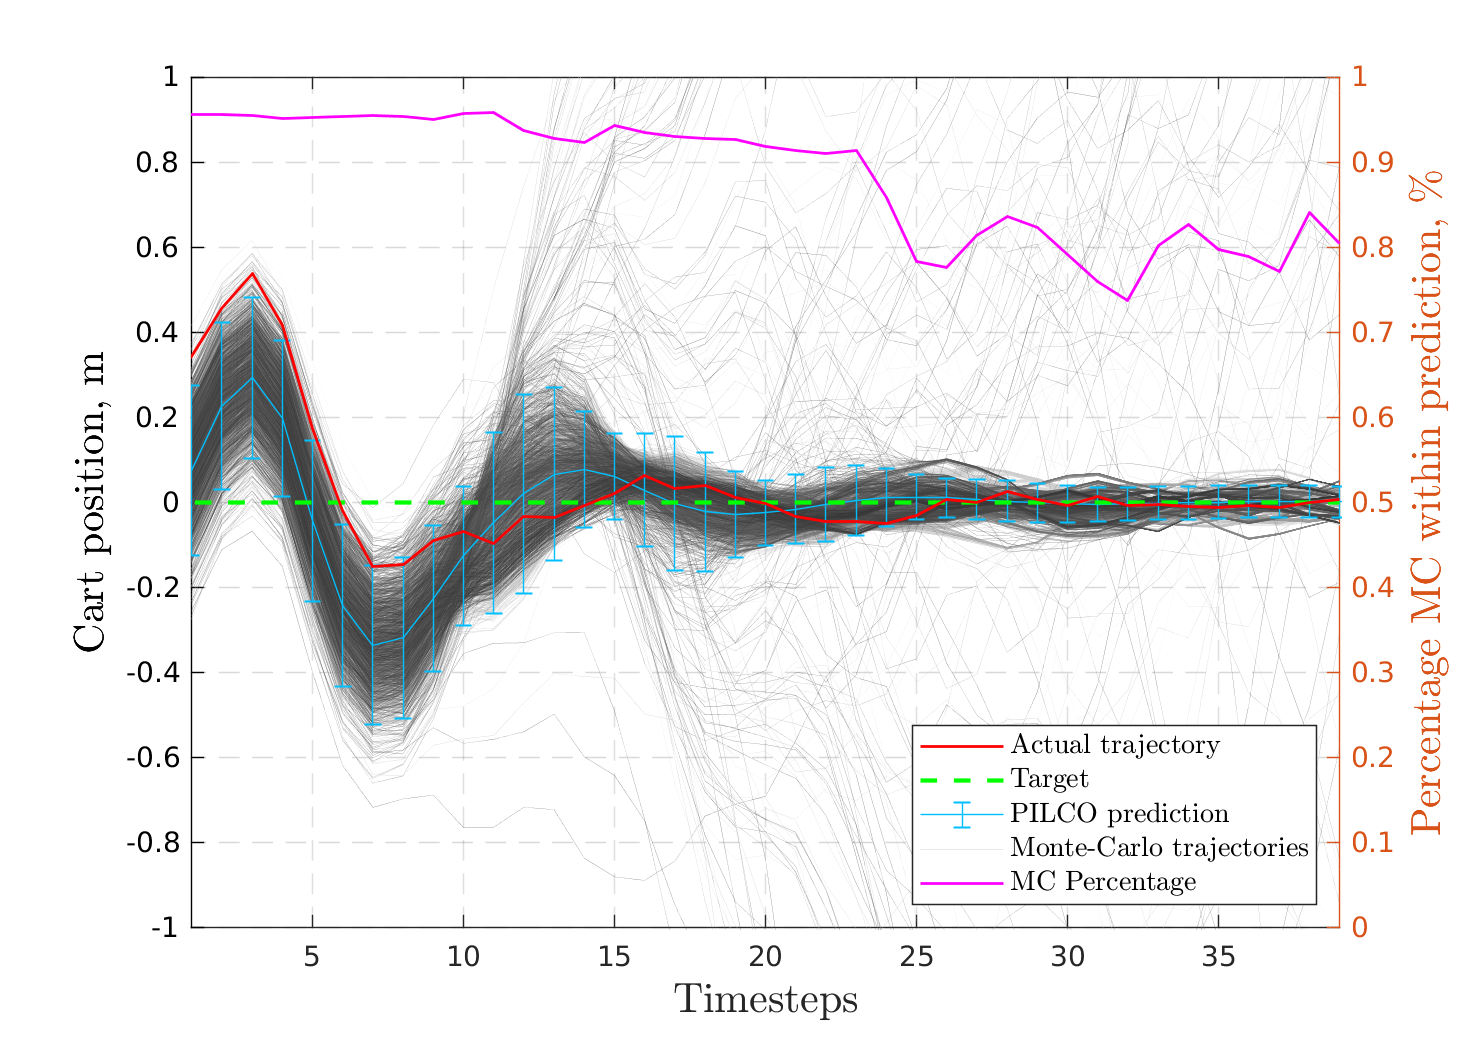
\includegraphics[height=0.4\textheight,width=1\textwidth]{Chapter3/Figures/cp_MC_rollout_Ep_15_Dim_1.png} 
    \caption{Cart position $x$ (m)} 
    \label{Fig:Re-cp-cart-position} 
  \end{subfigure} 
  \begin{subfigure}[b]{1\linewidth}
    \centering
    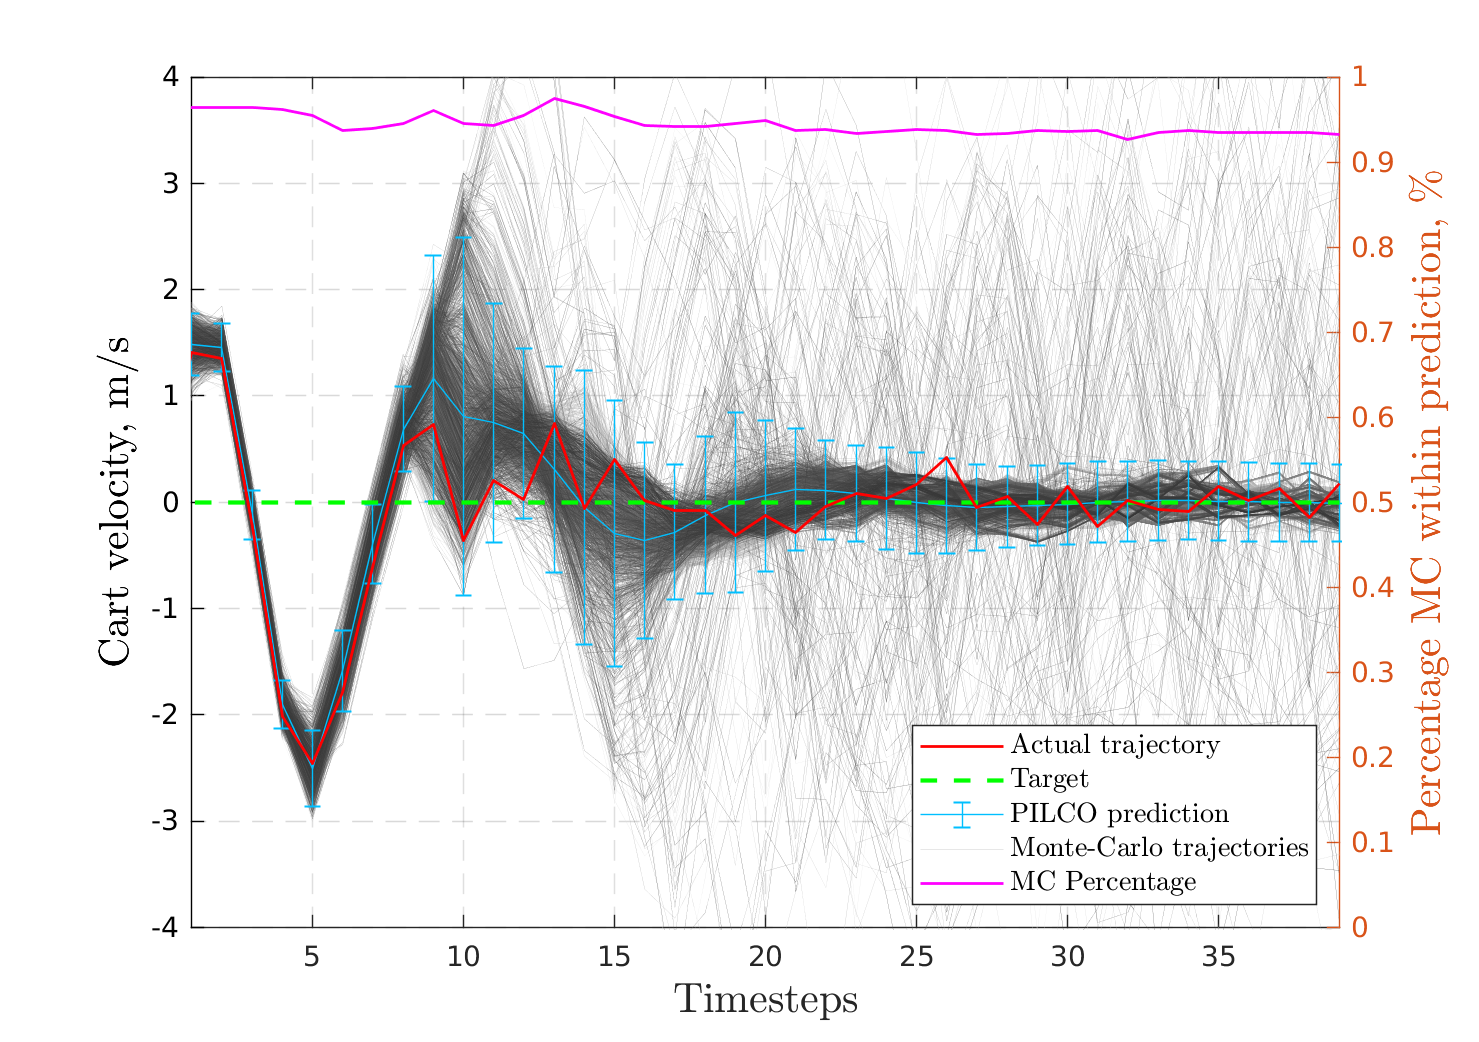
\includegraphics[height=0.4\textheight,width=1\textwidth]{Chapter3/Figures/cp_MC_rollout_Ep_15_Dim_2.png} 
    \caption{Cart velocity $\dot x$ (m/s)} 
    \label{Fig:Re-cp-cart-velocity} 
  \end{subfigure} 
\caption[Monte Carlo roll-outs for \textbf{cart-pole} cart position and cart velocity]{Monte Carlo roll-outs for the \textbf{cart-pole} environment for cart position and cart velocity. Figures show a random sample of the Monte Carlo trajectories for episode 15. The first three legend items (actual trajectory, target, PILCO prediction and MC trajectories) correspond to the state variable axis (left axis) and the magenta line shows the percentage of MC trajectories inside PILCO's prediction (2 standard deviations) (right axis). Sample time 0.1s, roll-out horizon 4.0s}
\label{Fig:Re-cp-MC-roll-outs-1} 
\end{figure}
 
 
\begin{figure}[htbp]    
  \begin{subfigure}[b]{1\linewidth}
    \centering
    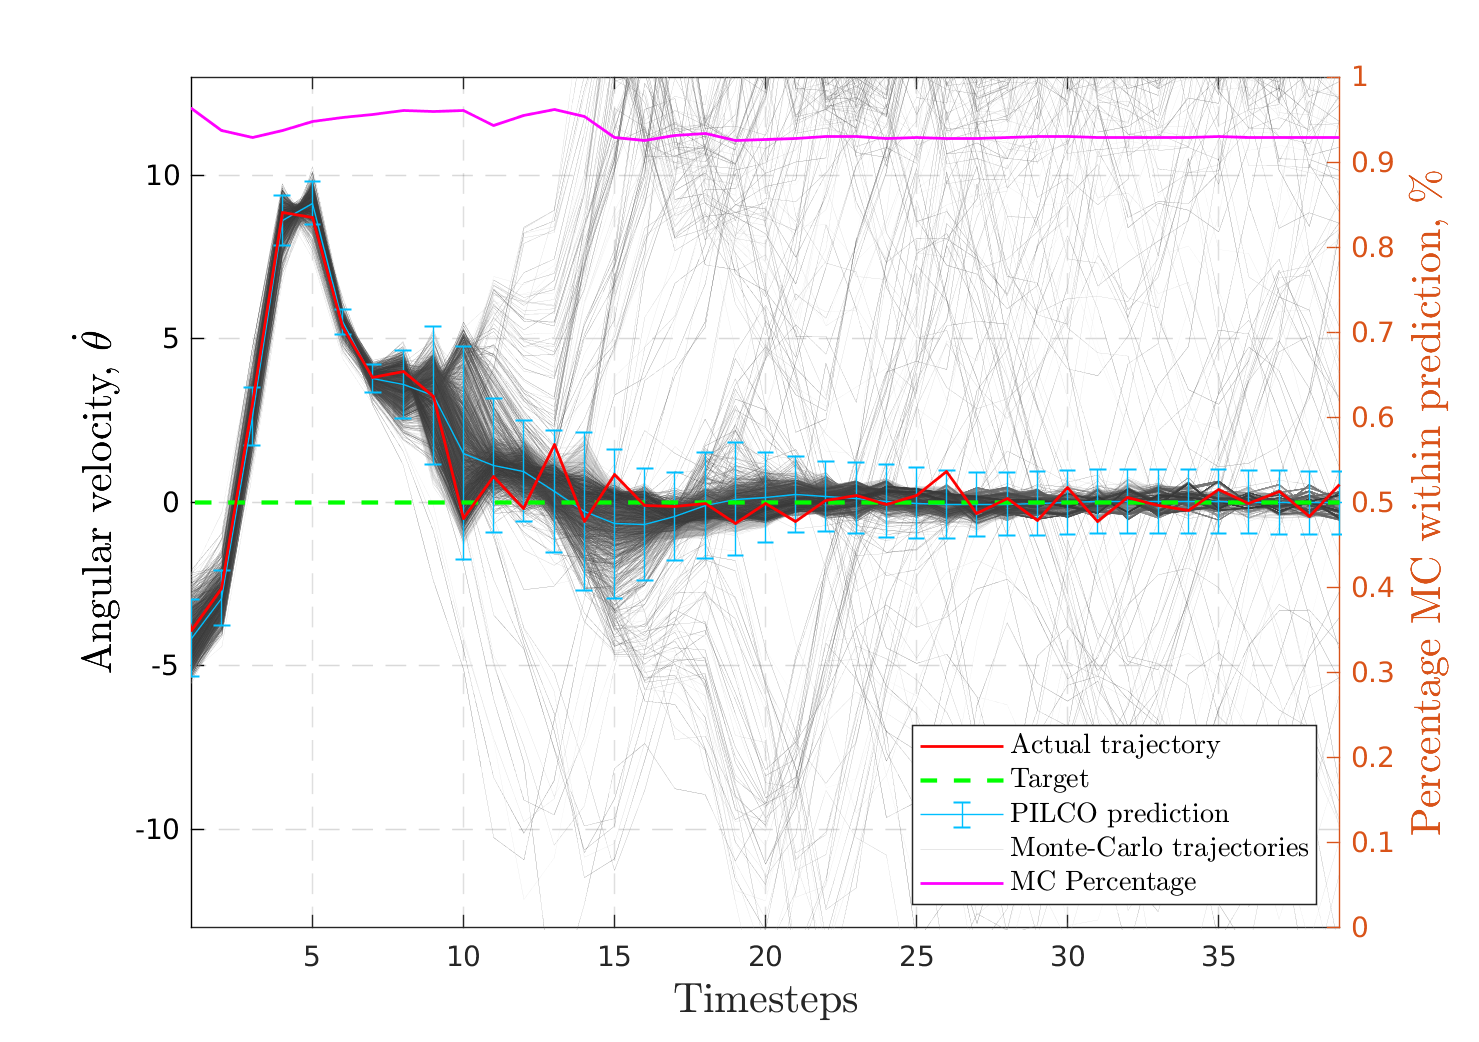
\includegraphics[height=0.4\textheight,width=1\textwidth]{Chapter3/Figures/cp_MC_rollout_Ep_15_Dim_3.png} 
    \caption{Pendulum angular velocity $\dot \theta$ (rad/s)} 
    \label{Fig:Re-cp-pen-velocity} 
  \end{subfigure} 

  \begin{subfigure}[b]{1\linewidth}
    \centering
    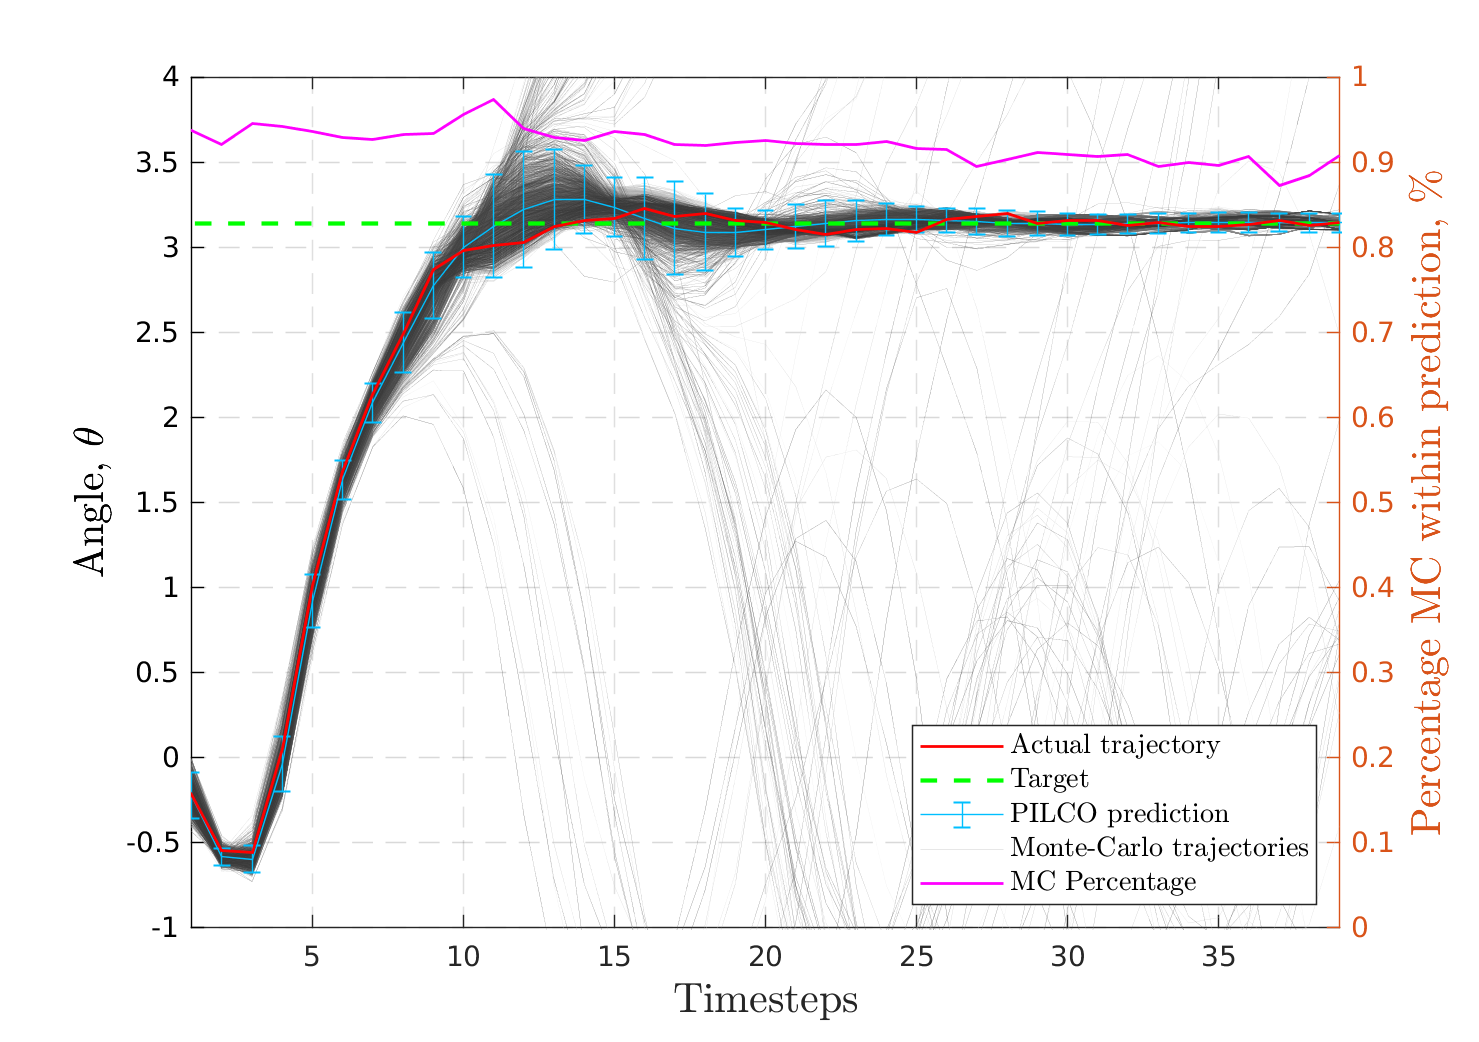
\includegraphics[height=0.4\textheight,width=1\textwidth]{Chapter3/Figures/cp_MC_rollout_Ep_15_Dim_4.png} 
    \caption{Pendulum angle $\theta$ (rad)} 
    \label{Fig:Re-cp-pen-angle} 
  \end{subfigure} 
\caption[Monte Carlo roll-outs for \textbf{cart-pole} pendulum angular velocity and pendulum angle]{Monte Carlo roll-outs for the \textbf{cart-pole} environment for pendulum angular velocity and pendulum angle. Figures show a random sample of the Monte Carlo trajectories for episode 15. The first three legend items (actual trajectory, target, PILCO prediction and MC trajectories) correspond to the state variable axis (left axis) and the magenta line shows the percentage of MC trajectories inside PILCO's prediction (2 standard deviations) (right axis). Sample time 0.1s, roll-out horizon 4.0s}
\label{Fig:Re-cp-MC-roll-outs-2} 
\end{figure}
 
\begin{figure}[htbp]    
  \begin{subfigure}[b]{1\linewidth}
    \centering
    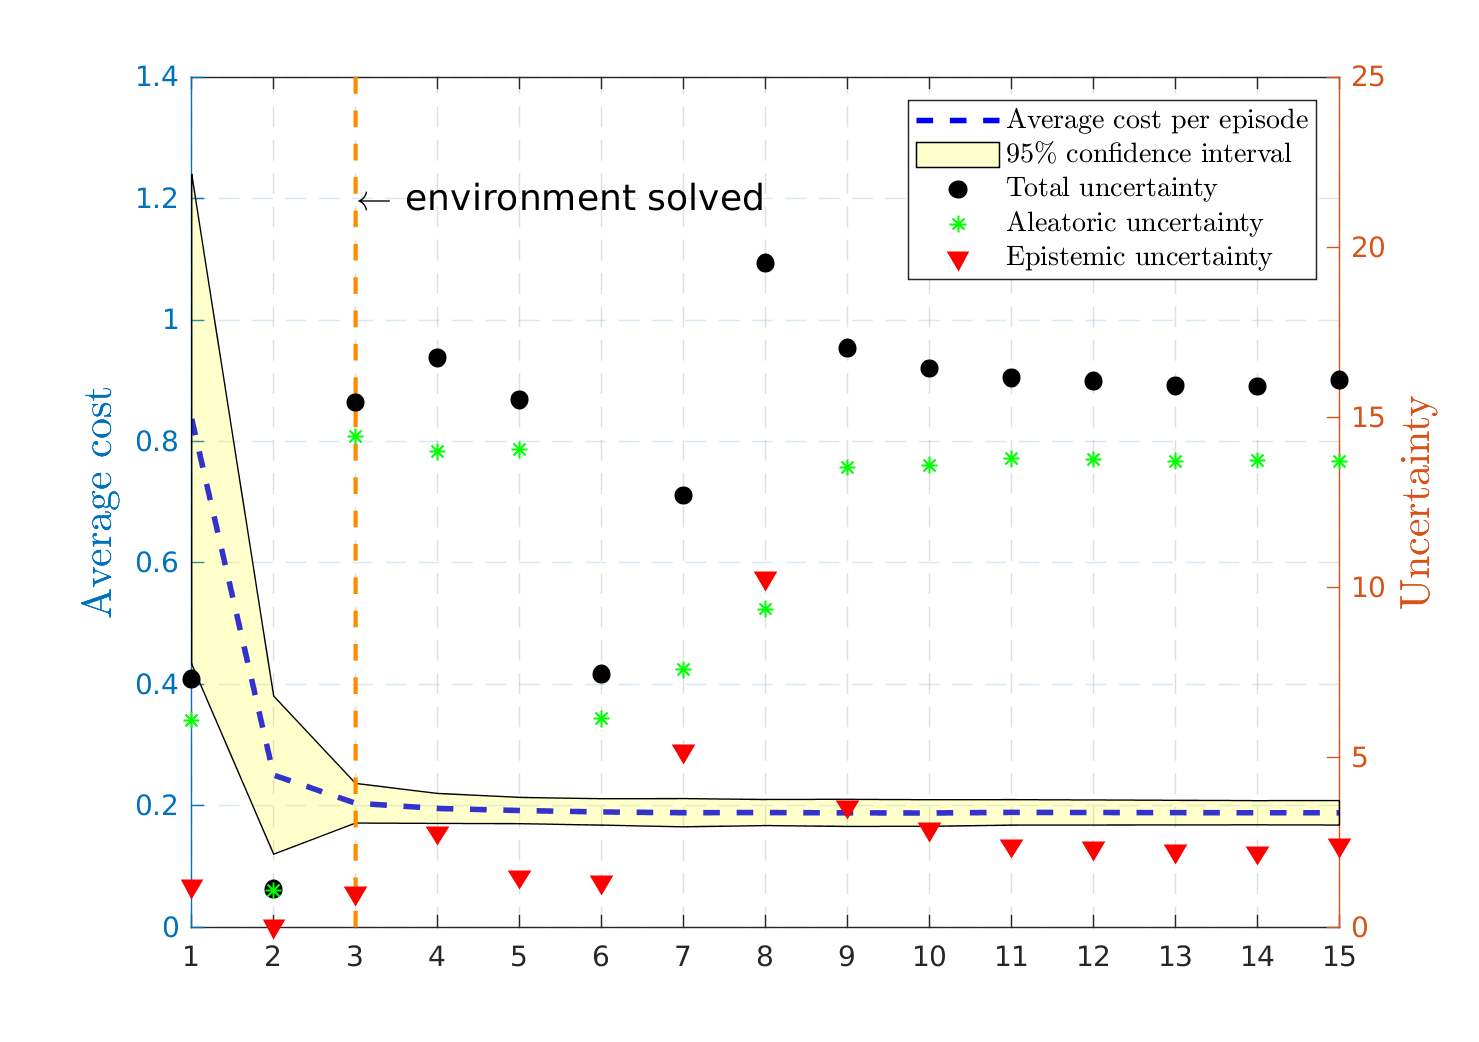
\includegraphics[height=0.4\textheight,width=1\textwidth]{Chapter3/Figures/cp_uncertainty.png} 
    \caption{Average cost (left axis) and uncertainty decomposition (right axis) for each episode over the course of learning.} 
    \label{Fig:Re-cp-uncertainty} 
  \end{subfigure}
  
  \begin{subfigure}[b]{1\linewidth}
    \centering
    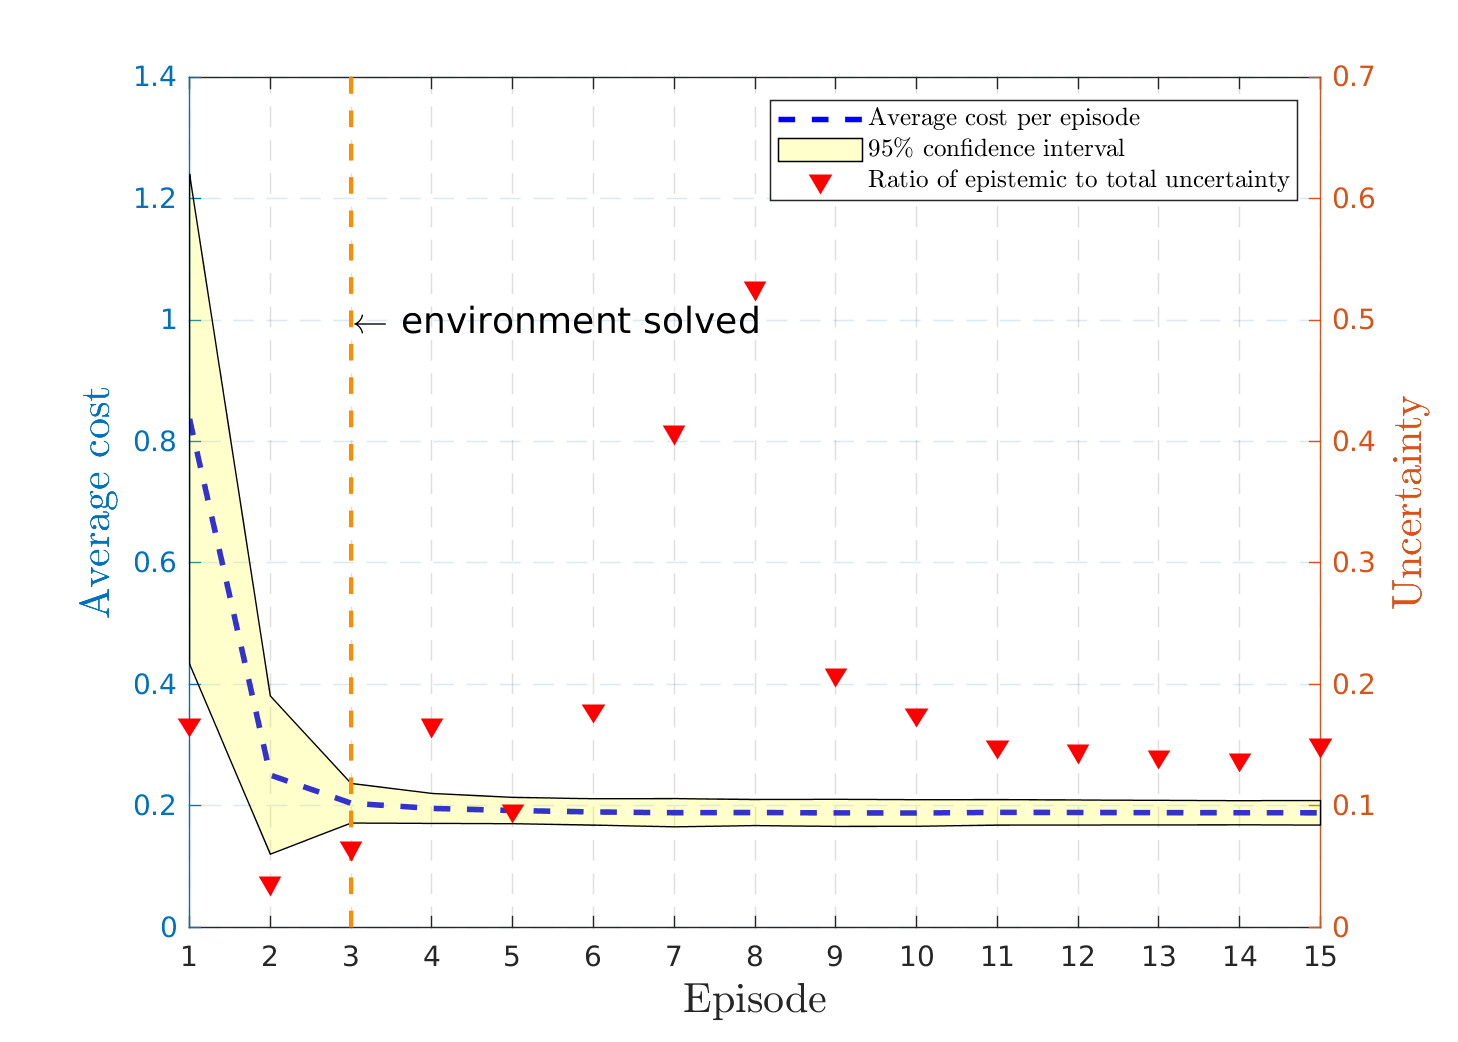
\includegraphics[height=0.4\textheight,width=1\textwidth]{Chapter3/Figures/cp_uncertainty_norm.png} 
    \caption{Average cost (left axis) and ratio of epistemic to total uncertainty (right axis) for each episode over the course of learning.} 
    \label{Fig:Re-cp-uncertainty-norm} 
  \end{subfigure}  
\caption[Uncertainty decomposition for \textbf{cart-pole} environment]{\textbf{Cart-pole}: Average cost (left axis) and uncertainty (right axis) for each episode over the course of learning.}
\label{Fig:Re-cp-full-uncertainty} 
\end{figure}
 
\subsubsection{Pendubot}
Fig. \ref{Fig:Re-pen-MC-roll-outs-1} and \ref{Fig:Re-pen-MC-roll-outs-2} show a random sample of the Monte Carlo trajectory roll-outs for the state variables of the pendubot environment: pendulum angular velocities $\dot{\theta}_{2}$, $\dot{\theta}_{3}$ and pendulum angles $\theta_{2}$, $\theta_{3}$. The trajectories shown in the figures are from episode 20, when PILCO has achieved the environment objective, and so represent trajectories under a mature policy $\pi$. Up to approximately 20 time steps there is cohesion in the Monte Carlo trajectories which corresponds to the period where the pendulums are being manoeuvred to the upright position. After this, the trajectories spread out which corresponds to the period where the agent attempts to balance the pendulums in the upright position. This indicates that there is more uncertainty in the policy during the balancing phase than during the swing-up phase. Although there is a large amount of spread in the trajectories, approximately $70\%$ are still within PILCO's 2 standard deviation prediction. 

Fig. \ref{Fig:Re-pen-full-uncertainty} shows the average cost per episode and the uncertainty in the cost over the course of learning. Starting with Fig. \ref{Fig:Re-pen-uncertainty}. Over the first five episodes, the agent learns to swing the pendulums to the upright position but cannot keep them balance. During this phase, the average cost steps down from its initial value and consequently the total and aleatoric uncertainties in the cost increase while the epistemic cost uncertainty remains low. The increase in total cost uncertainty is due to the agent forming an initial belief about the environment (with no belief there is no uncertainty). Over the course of the next 10 episodes, the agent learns to maintain the balance of the pendulums. Again a step down in average cost is observed and this time an increase in aleatoric, epistemic and total cost uncertainty is observed. Once the environment is solved, the aleatoric cost uncertainty stabilises and the epistemic cost uncertainty reduces. From this representation, it is difficult to see the how the breakdown of cost uncertainties relate to learning. 

In Fig. \ref{Fig:Re-pen-uncertainty-norm}, the cost uncertainty is represented as the ratio of epistemic to total uncertainty. The first three episodes each yield an average cost of approximately 0.95 indicating that little learning is occurring over this period. During these episodes, PILCO has selected policies that have a low ratio of epistemic to total cost uncertainty. From episodes 3 to 4, the average cost reduces from 0.95 to 0.83 and this step in learning corresponds to a policy which has a higher ratio of epistemic to total cost uncertainty than the previous episodes. This trend repeats for episodes 5, 6 and 7 where the average cost plateaus for 5 and 6, corresponding to policies with a low ratio of epistemic to total cost uncertainty, but reduces for episode 7, corresponding to a policy with a high ratio of epistemic to total cost uncertainty. Perhaps the most convincing demonstration of this correlation occurs between episodes 7 and 8 where the largest observed step decrease in average cost occurs and corresponds to a policy with the largest ratio of epistemic to total cost uncertainty. Finally, after the environment is solved around episode 8, the ratio of epistemic to total cost uncertainty drops off as the agent refines the policy and model confidence increases. 

 \begin{figure}[htbp]    
    \begin{subfigure}[b]{1\linewidth}
    \centering
    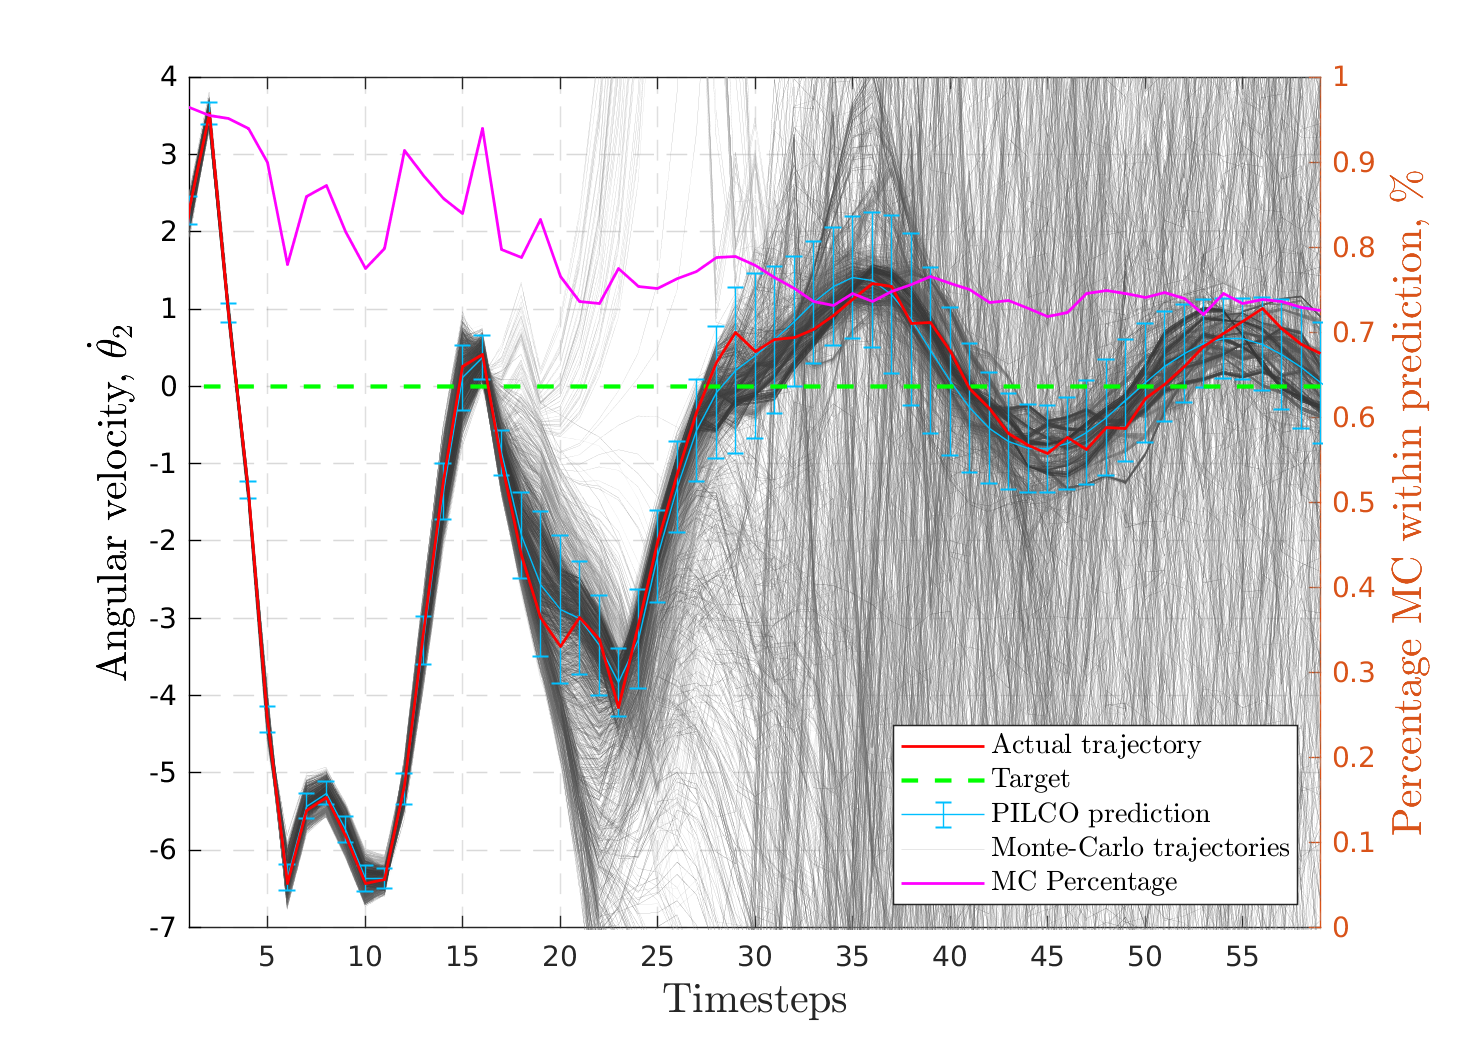
\includegraphics[height=0.4\textheight,width=1\textwidth]{Chapter3/Figures/pen_MC_rollout_Ep_40_Dim_1.png} 
    \caption{Pendulum angular velocity $\dot \theta_{2}$ (rad/s)} 
    \label{Fig:Re-pen-cart-position} 
  \end{subfigure} 
  \hspace{\fill}  %% maximize space between adjacent subfigures
  \begin{subfigure}[b]{1\linewidth}
    \centering
    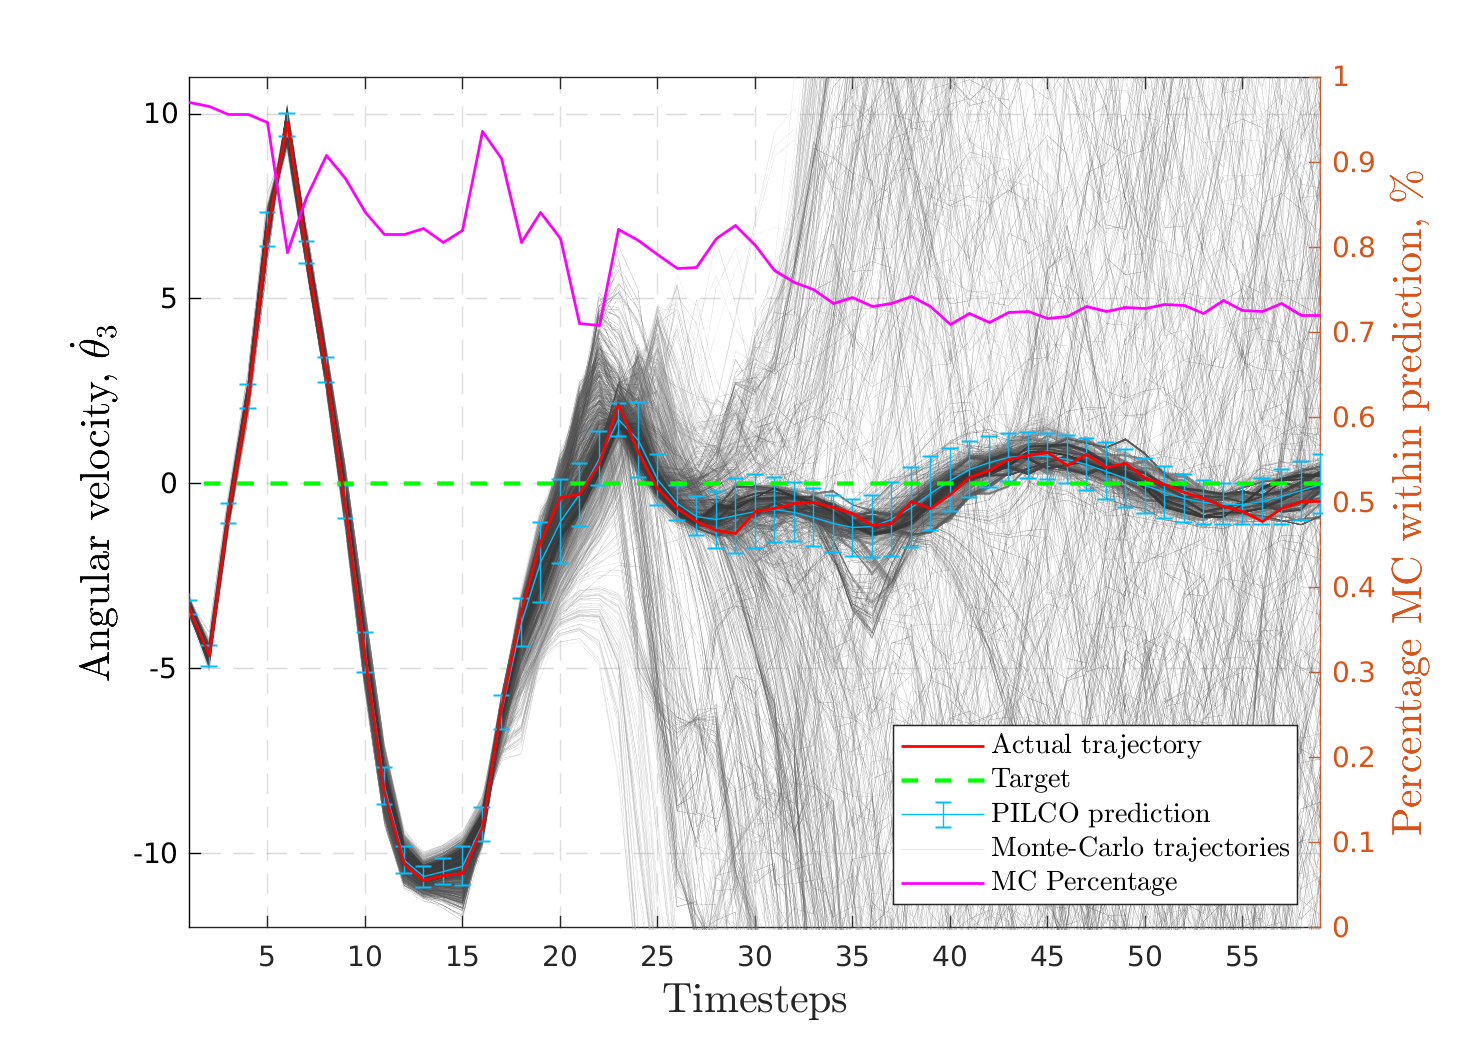
\includegraphics[height=0.4\textheight,width=1\textwidth]{Chapter3/Figures/pen_MC_rollout_Ep_40_Dim_2.png} 
    \caption{Pendulum angular velocity $\dot \theta_{3}$ (rad/s)} 
    \label{Fig:Re-pen-cart-velocity} 
  \end{subfigure} 
\caption[Monte Carlo roll-outs for \textbf{pendubot} pendulum angular velocities]{Monte Carlo roll-outs for the \textbf{pendubot} environment for pendulum angular velocities. Figures show a random sample of the Monte Carlo trajectories for episode 20. The first three legend items (actual trajectory, target, PILCO prediction and MC trajectories) correspond to the state variable axis (left axis) and the magenta line shows the percentage of MC trajectories inside PILCO's prediction (2 standard deviations) (right axis). Sample time 0.05s, roll-out horizon 3.0s.}
\label{Fig:Re-pen-MC-roll-outs-1} 
\end{figure}
 
 
\begin{figure}[htbp]    
   \begin{subfigure}[b]{1\linewidth}
    \centering
    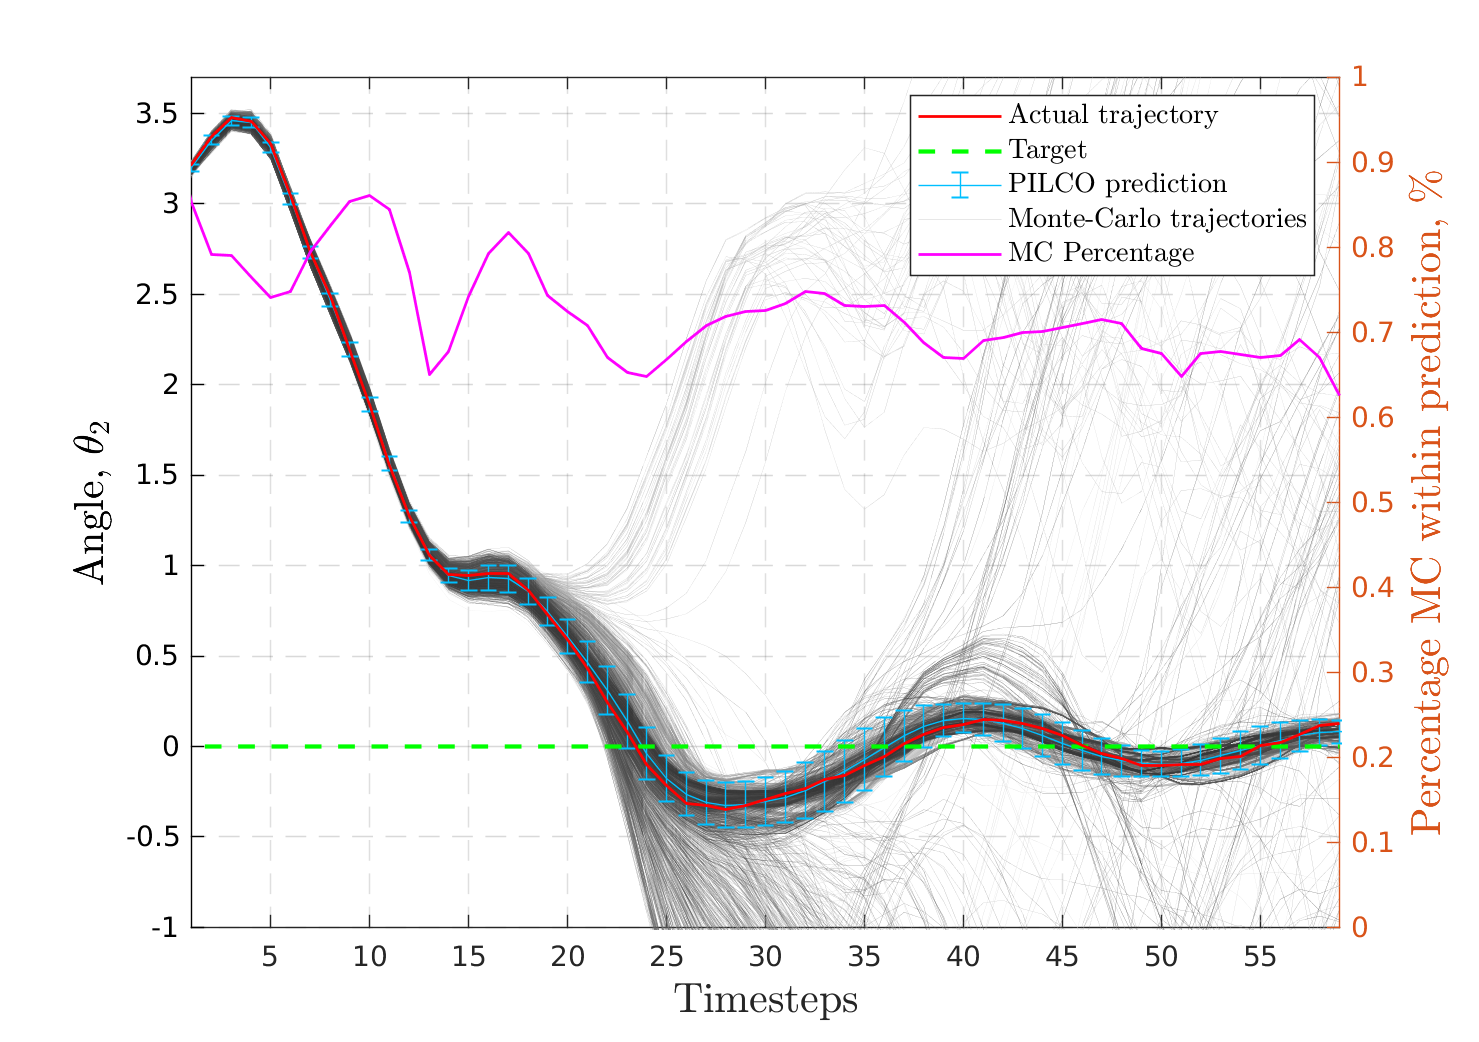
\includegraphics[height=0.4\textheight,width=1\textwidth]{Chapter3/Figures/pen_MC_rollout_Ep_40_Dim_3.png} 
    \caption{Pendulum angle $\theta_2$ (rad)} 
    \label{Fig:Re-pen-pen-velocity} 
  \end{subfigure} 
  \hspace{\fill}
  \begin{subfigure}[b]{1\linewidth}
    \centering
    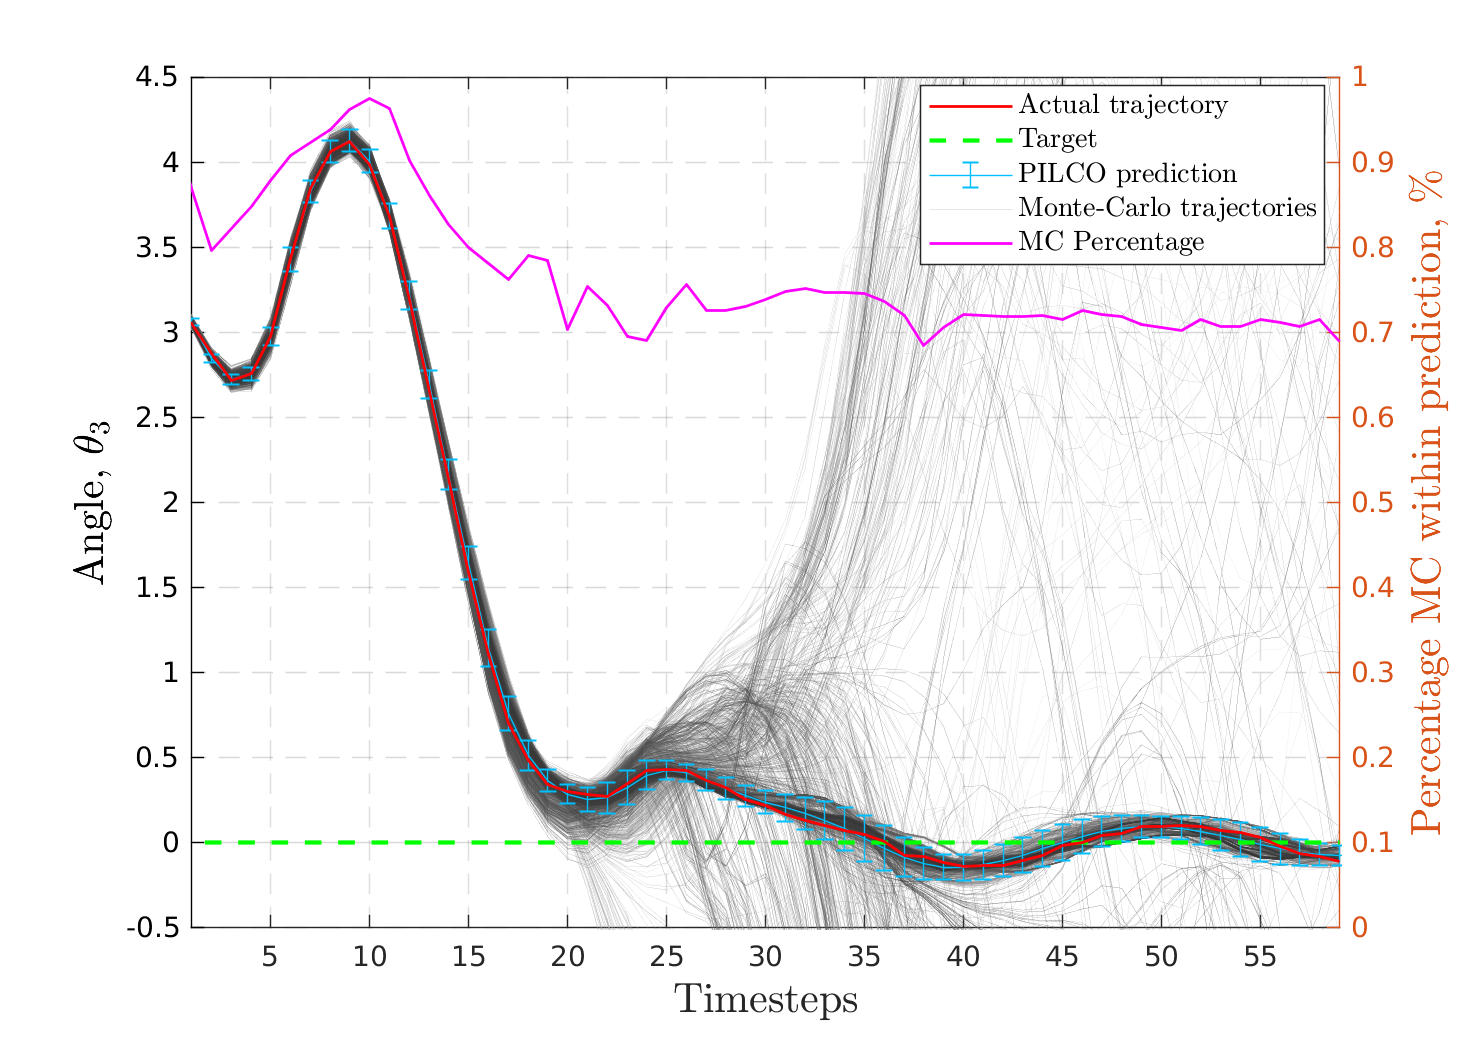
\includegraphics[height=0.4\textheight,width=1\textwidth]{Chapter3/Figures/pen_MC_rollout_Ep_40_Dim_4.png} 
    \caption{Pendulum angle $\theta_3$ (rad)} 
    \label{Fig:Re-pen-pen-angle} 
  \end{subfigure} 

\caption[Monte Carlo roll-outs for \textbf{pendubot} pendulum angles]{Monte Carlo roll-outs for the \textbf{pendubot} environment for pendulum angles. Figures show a random sample of the Monte Carlo trajectories for episode 20. The first three legend items (actual trajectory, target, PILCO prediction and MC trajectories) correspond to the state variable axis (left axis) and the magenta line shows the percentage of MC trajectories inside PILCO's prediction (2 standard deviations) (right axis). Sample time 0.05s, roll-out horizon 3.0s.}
\label{Fig:Re-pen-MC-roll-outs-2} 
\end{figure}
 
\begin{figure}[htbp]    
   \begin{subfigure}[b]{1\linewidth}
    \centering
    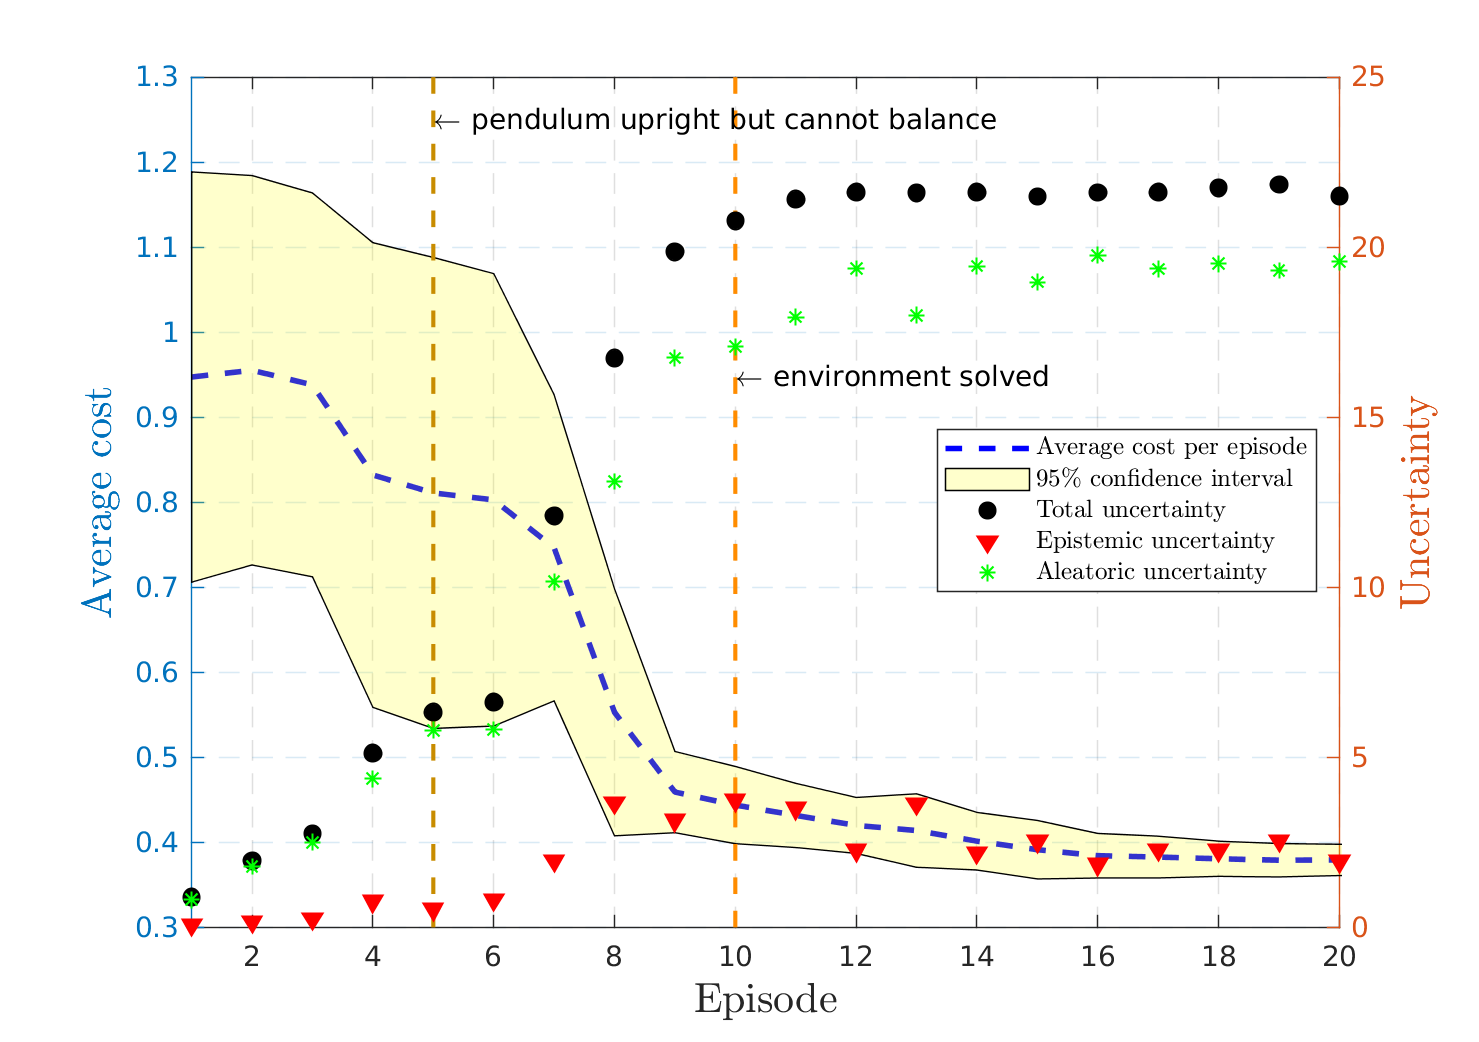
\includegraphics[height=0.4\textheight,width=1\textwidth]{Chapter3/Figures/pen_uncertainty.png} 
    \caption{Average cost (left axis) and uncertainty decomposition (right axis) for each episode over the course of learning.} 
    \label{Fig:Re-pen-uncertainty} 
  \end{subfigure}
  \hspace{\fill}
  \begin{subfigure}[b]{1\linewidth}
    \centering
    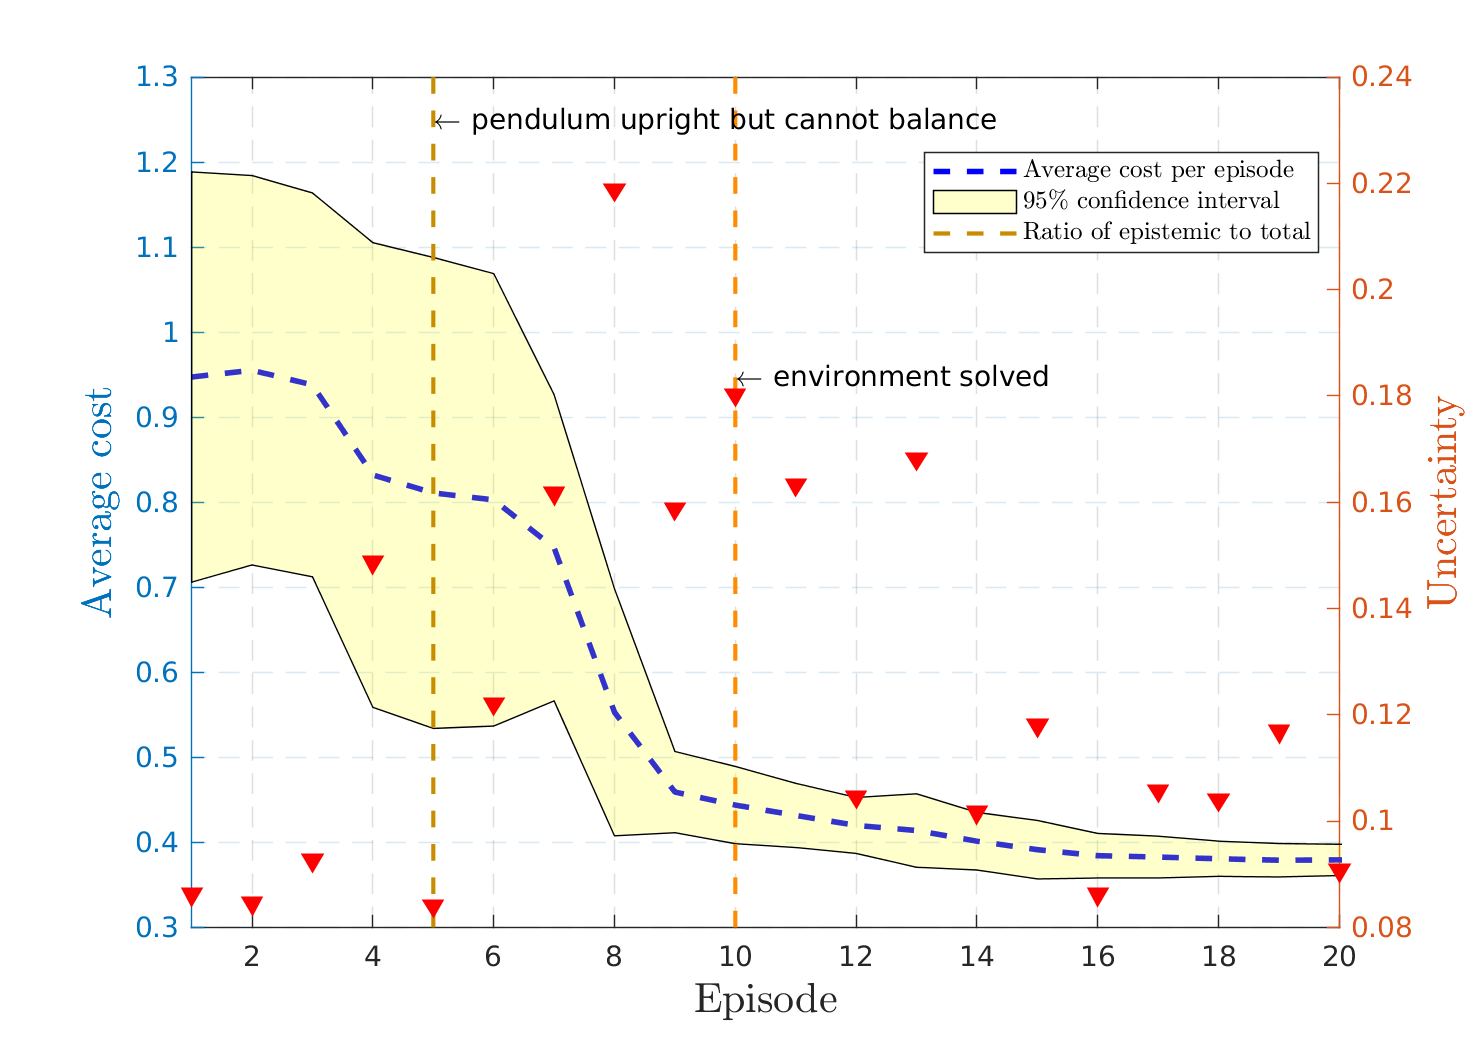
\includegraphics[height=0.4\textheight,width=1\textwidth]{Chapter3/Figures/pen_uncertainty_norm.png} 
    \caption{Average cost (left axis) and ratio of epistemic to total uncertainty (right axis) for each episode over the course of learning.} 
    \label{Fig:Re-pen-uncertainty-norm} 
  \end{subfigure} 
\caption[Uncertainty decomposition for \textbf{pendubot} environment]{\textbf{Pendubot}: Average cost (left axis) and uncertainty (right axis) for each episode over the course of learning.}
\label{Fig:Re-pen-full-uncertainty} 
\end{figure}


\subsubsection{Cart-Double-Pendulum}
Fig. \ref{Fig:Re-cdp-MC-roll-outs-1} - \ref{Fig:Re-cdp-MC-roll-outs-3} show a random sample of the Monte Carlo trajectory roll-outs for the state variables of the cart-double-pendulum environment: cart position $x$, cart velocity $\dot x$, pendulum angular velocities $\dot{\theta}_{2}$, $\dot{\theta}_{3}$ and pendulum angles $\theta_{2}$, $\theta_{3}$. The trajectories shown in the figures are from episode 80, when PILCO has achieved the environment objective, and so represent trajectories under a mature policy $\pi$. Up to approximately 30 time steps there is cohesion in the Monte Carlo trajectories which again corresponds to the swing-up phase. During the balance phase, the trajectories spread out. By the end of the episode, only about $40\%$ of the trajectories fall within PILCO's predictions. 

Fig. \ref{Fig:Re-cdp-full-uncertainty} shows the average cost per episode and the uncertainty in the cost over the course of learning. Starting with Fig. \ref{Fig:Re-cdp-uncertainty}. After 10 episodes, the agent has learned to swing the pendulums into the upright position but cannot yet maintain them in a balanced state. During this phase there is a small reduction in average cost. The agent then takes a further 33 episodes to learn to maintain the pendulums in a balanced but off-centre position. During this second phase of learning, the total and epistemic cost uncertainties increase as the agent forms a belief about the environment, however, policies associated with low epistemic cost uncertainty are consistently being selected. Consequently, the learning gradient is gentle. Just after 40 episodes, there is a rapid increase in learning. During this phase, the total cost uncertainty rises further and departs from the trend  of the aleatoric cost uncertainty due to the increase in epistemic cost uncertainty. 

Fig. \ref{Fig:Re-cdp-uncertainty-normalised} shows a more pronounced trend in the ratio of total to epistemic cost uncertainty. Approaching the 40 episode mark, PILCO selects policies with an increasing ratio of total to epistemic cost uncertainty and as a consequence learning increases. Here there is a clear correlation between the amount of epistemic cost uncertainty present in the policy and the average cost. This shows that policies with a high epistemic cost uncertainty lead to a steeper learning gradient. 

 \begin{figure}[htbp]    
    \begin{subfigure}[b]{1\linewidth}
    \centering
    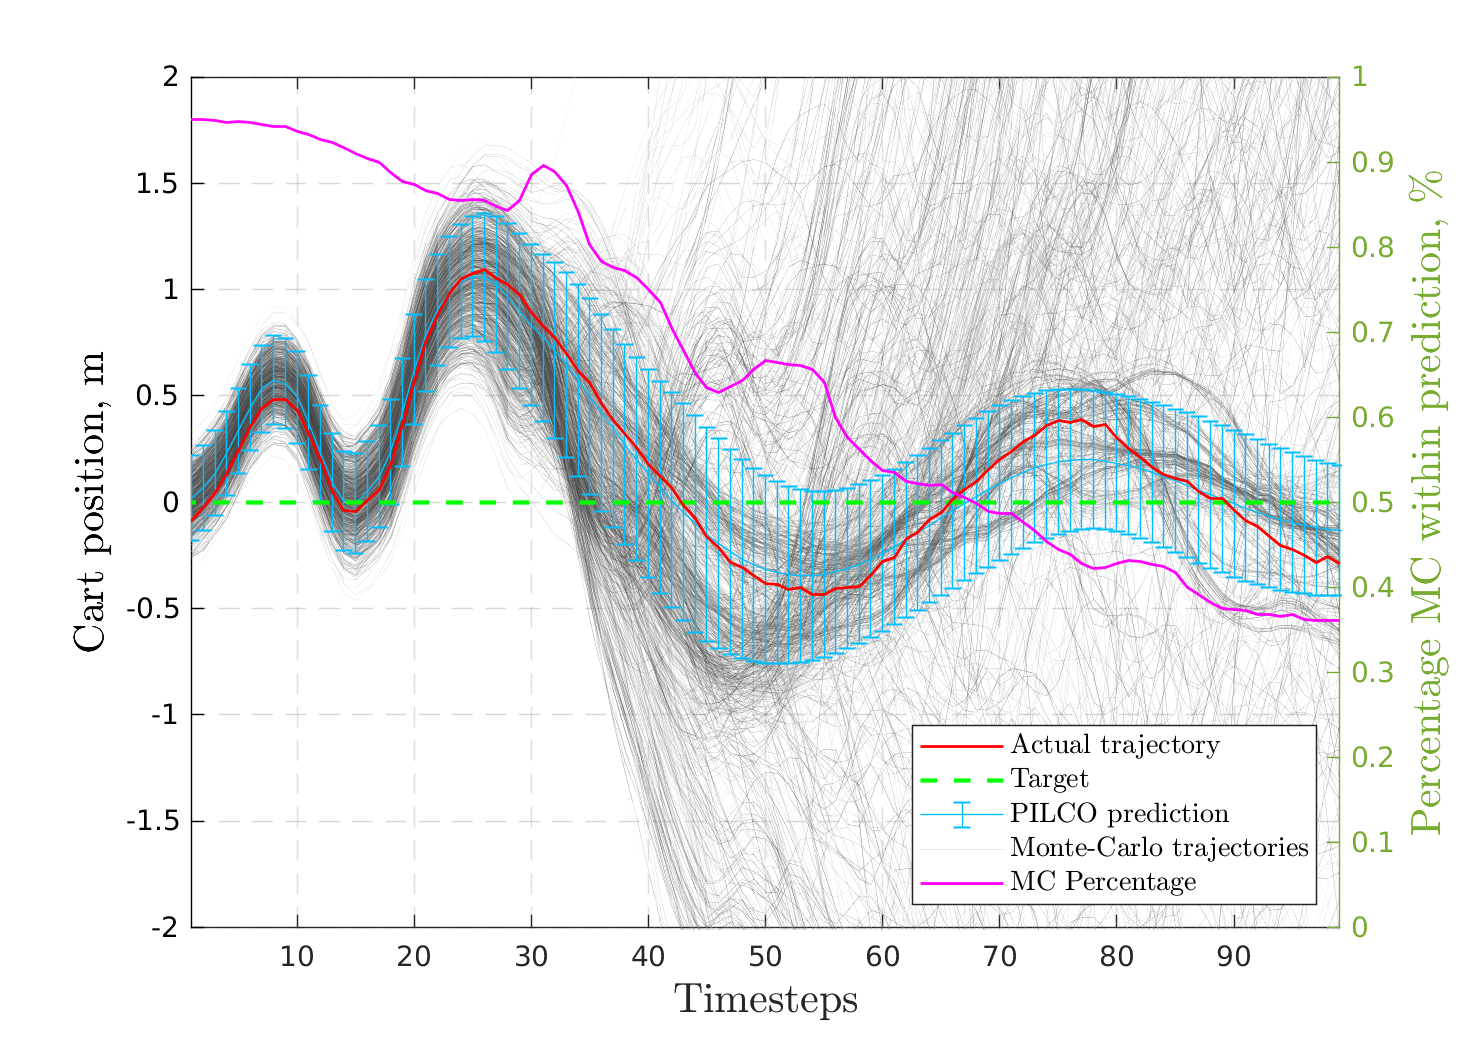
\includegraphics[height=0.4\textheight,width=1\textwidth]{Chapter3/Figures/cdp_MC_rollout_Ep_80_Dim_1.png} 
    \caption{Cart position $x_1$ (m)} 
    \label{Fig:Re-cdp-cart-position} 
  \end{subfigure} 

  \begin{subfigure}[b]{1\linewidth}
    \centering
    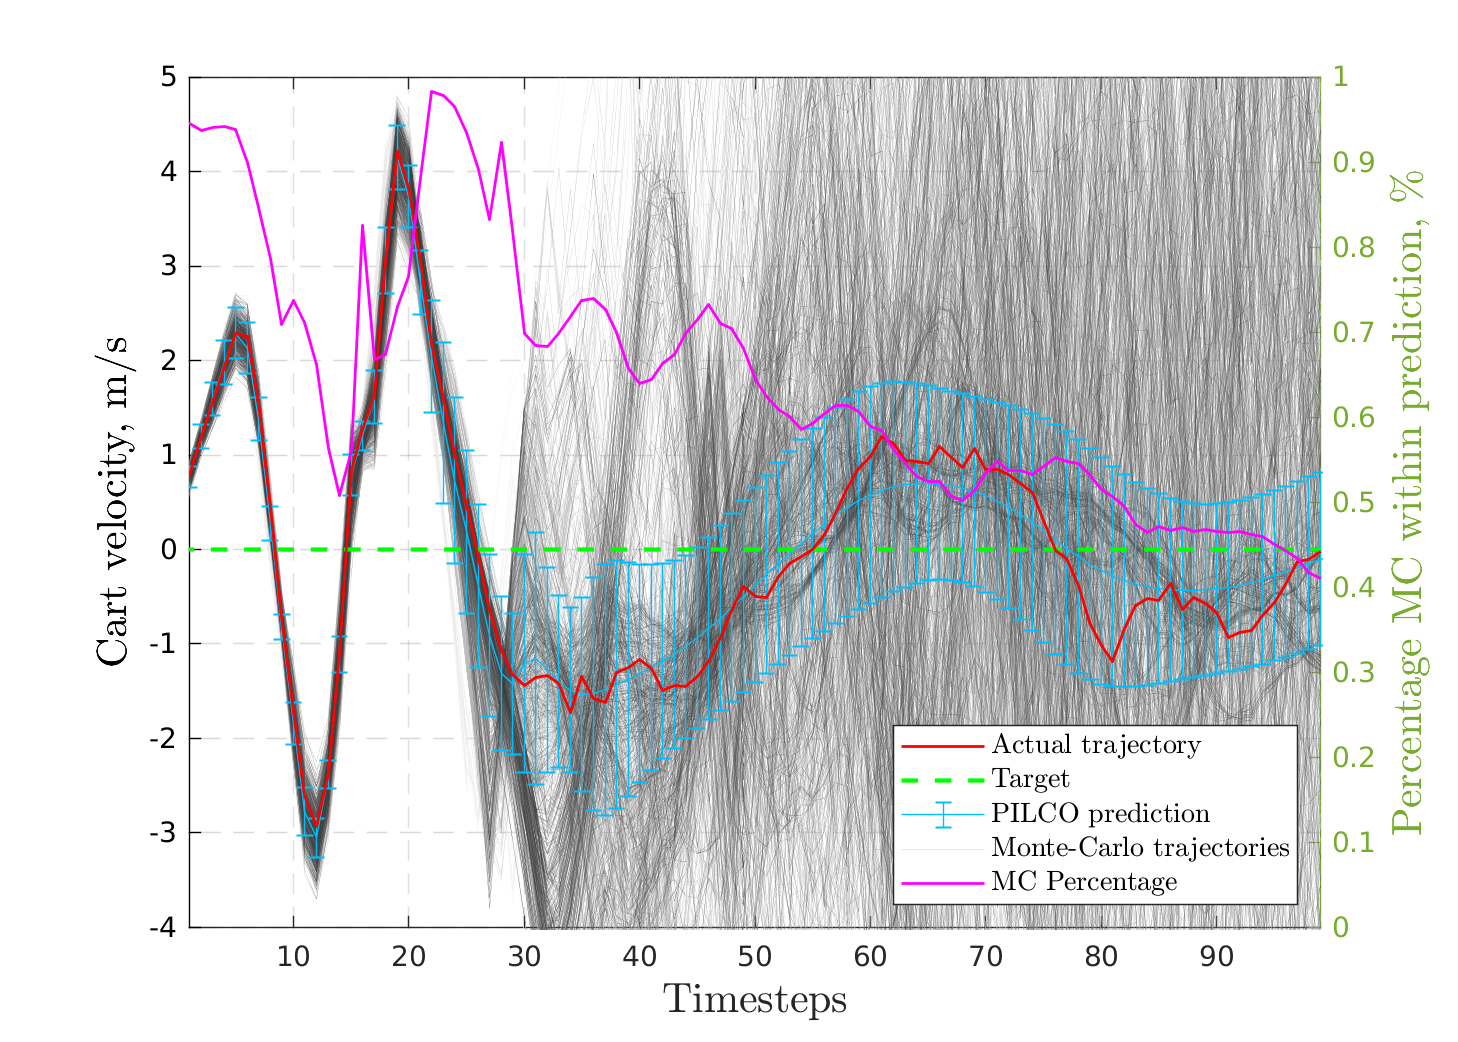
\includegraphics[height=0.4\textheight,width=1\textwidth]{Chapter3/Figures/cdp_MC_rollout_Ep_80_Dim_2.png} 
    \caption{Cart velocity $\dot{x}_1$ (m/s)} 
    \label{Fig:Re-cdp-cart-velocity} 
  \end{subfigure} 
\caption[Monte Carlo roll-outs for \textbf{cart-double-pendulum} cart position and cart velocity]{Monte Carlo roll-outs for the \textbf{cart-double-pendulum} environment for cart position and cart velocity. Figures show a random sample of the Monte Carlo trajectories for episode 75. The first three legend items (actual trajectory, target, PILCO prediction and MC trajectories) correspond to the state variable axis (left axis) and the magenta line shows the percentage of MC trajectories inside PILCO's prediction (2 standard deviations) (right axis). Sample time 0.05s, roll-out horizon 5.0s.}
\label{Fig:Re-cdp-MC-roll-outs-1} 
\end{figure}
 
 
\begin{figure}[htbp]    
   \begin{subfigure}[b]{1\linewidth}
    \centering
    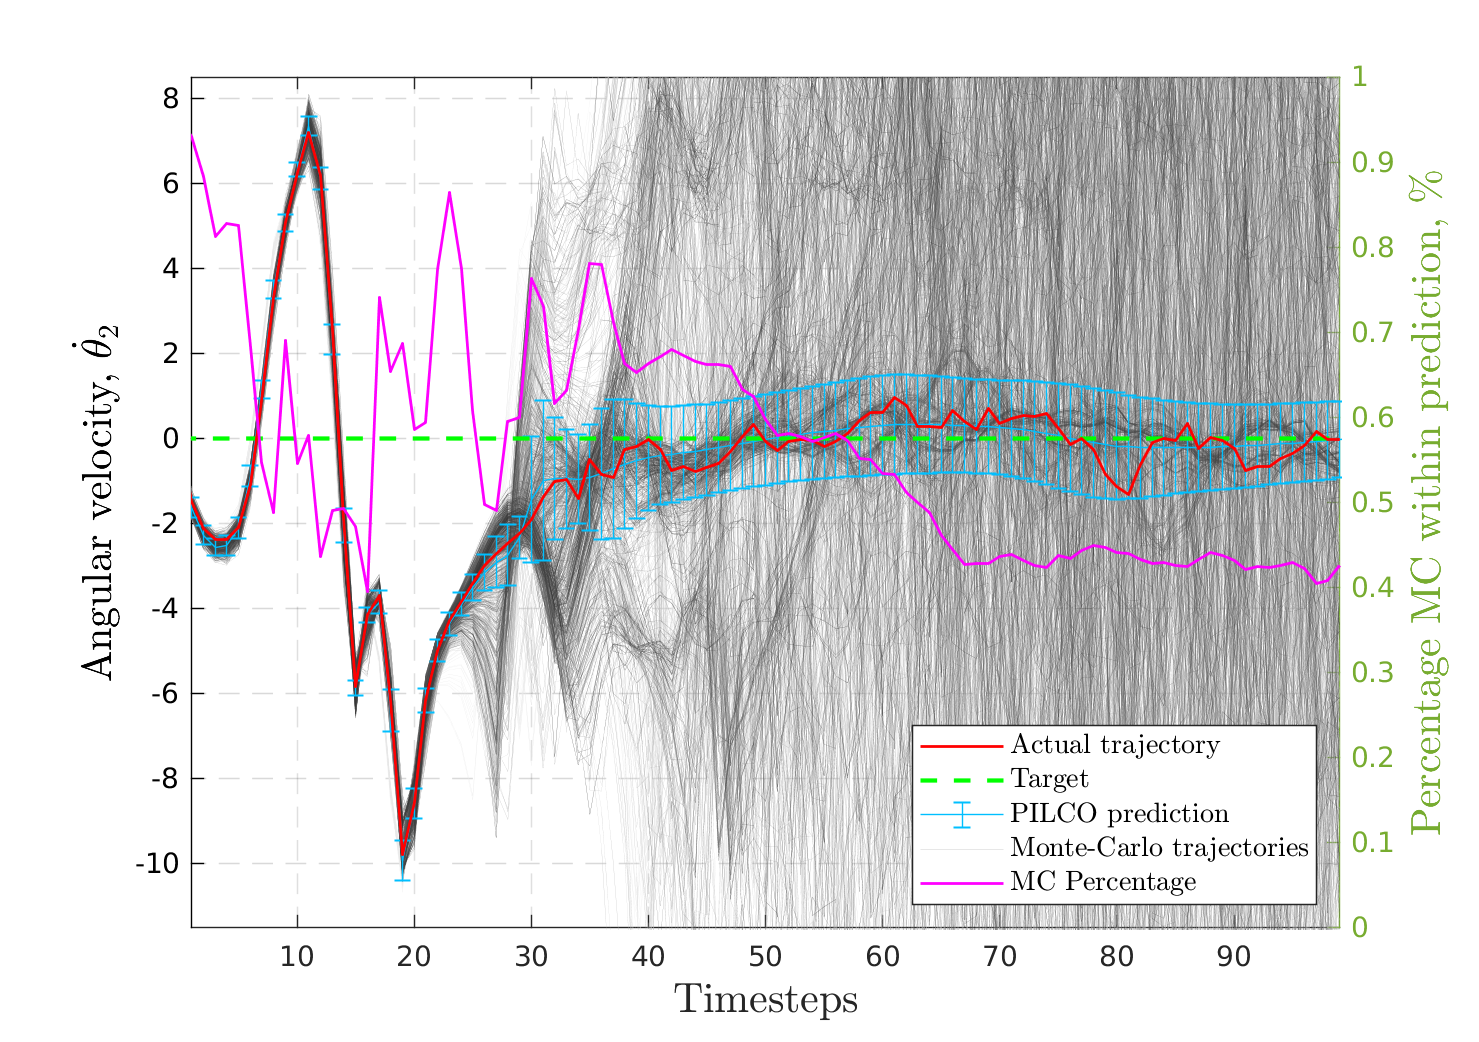
\includegraphics[height=0.4\textheight,width=1\textwidth]{Chapter3/Figures/cdp_MC_rollout_Ep_80_Dim_3.png} 
    \caption{Pendulum angular velocity $\dot{\theta}_2$ (rad/s)} 
    \label{Fig:Re-cdp-pen2-velocity} 
  \end{subfigure} 
  \hspace{\fill}
  \begin{subfigure}[b]{1\linewidth}
    \centering
    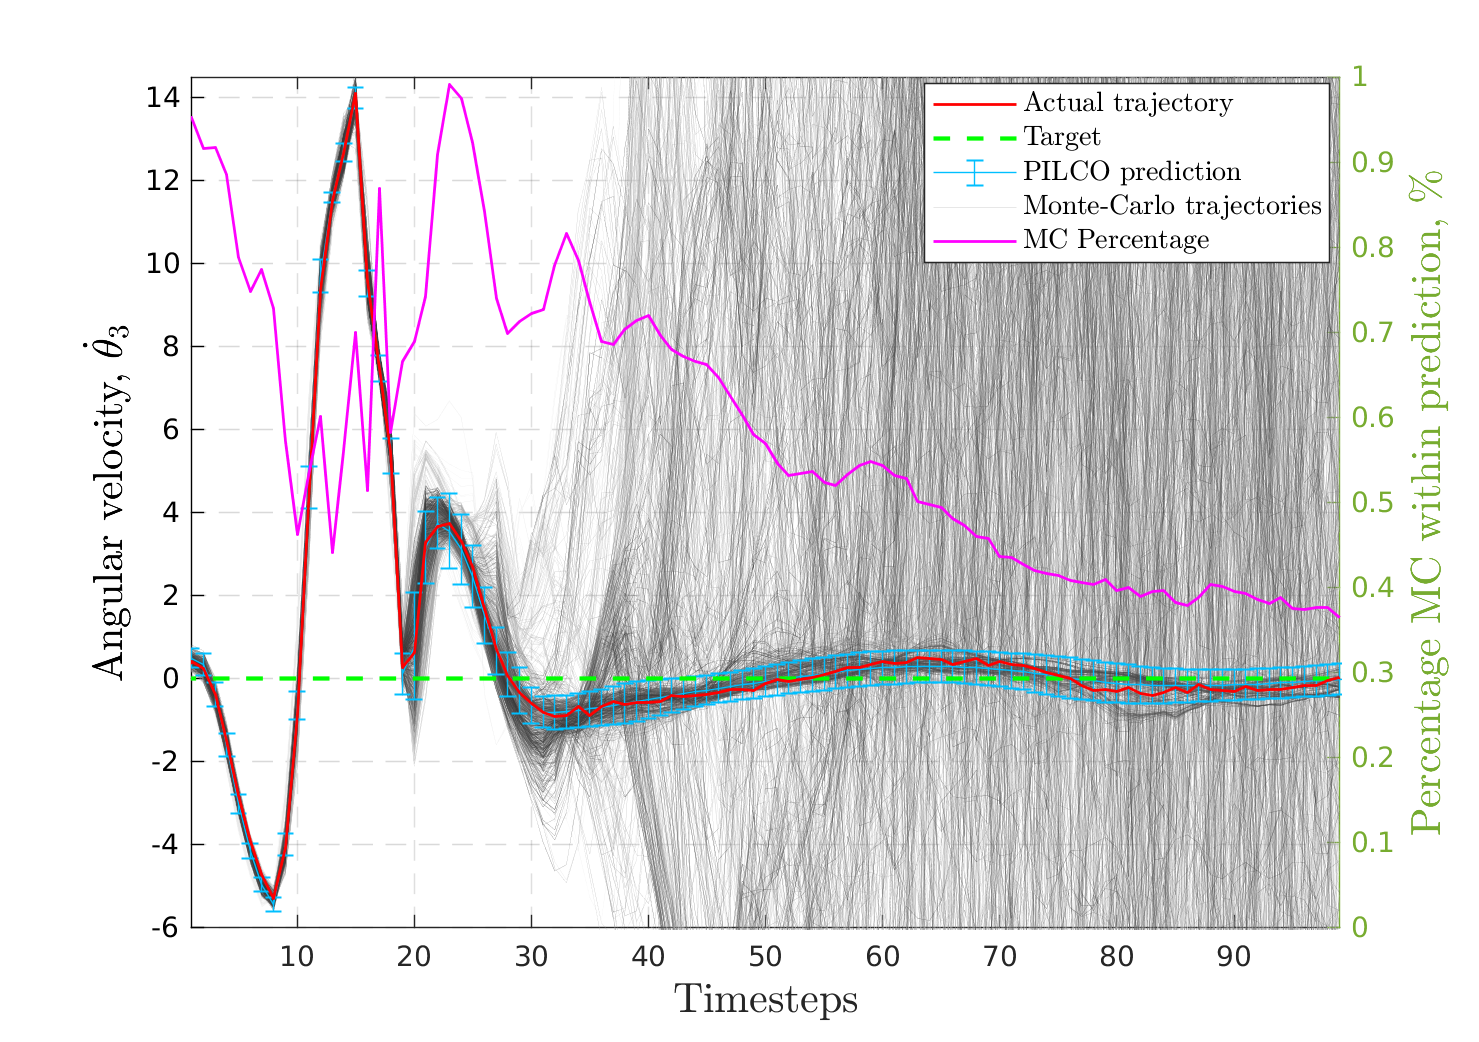
\includegraphics[height=0.4\textheight,width=1\textwidth]{Chapter3/Figures/cdp_MC_rollout_Ep_80_Dim_4.png} 
    \caption{Pendulum angular velocity $\dot{\theta}_3$ (rad/s)} 
    \label{Fig:Re-cdp-pen3-velocity} 
  \end{subfigure} 

\caption[Monte Carlo roll-outs for \textbf{cart-double-pendulum} pendulum angular velocities]{Monte Carlo roll-outs for the \textbf{cart-double-pendulum} environment for  pendulum angular velocities]. Figures show a random sample of the Monte Carlo trajectories for episode 75. The first three legend items (actual trajectory, target, PILCO prediction and MC trajectories) correspond to the state variable axis (left axis) and the magenta line shows the percentage of MC trajectories inside PILCO's prediction (2 standard deviations) (right axis). Sample time 0.05s, roll-out horizon 5.0s.}
\label{Fig:Re-cdp-MC-roll-outs-2} 
\end{figure}
 
\begin{figure}[htbp]    
    \begin{subfigure}[b]{1\linewidth}
    \centering
    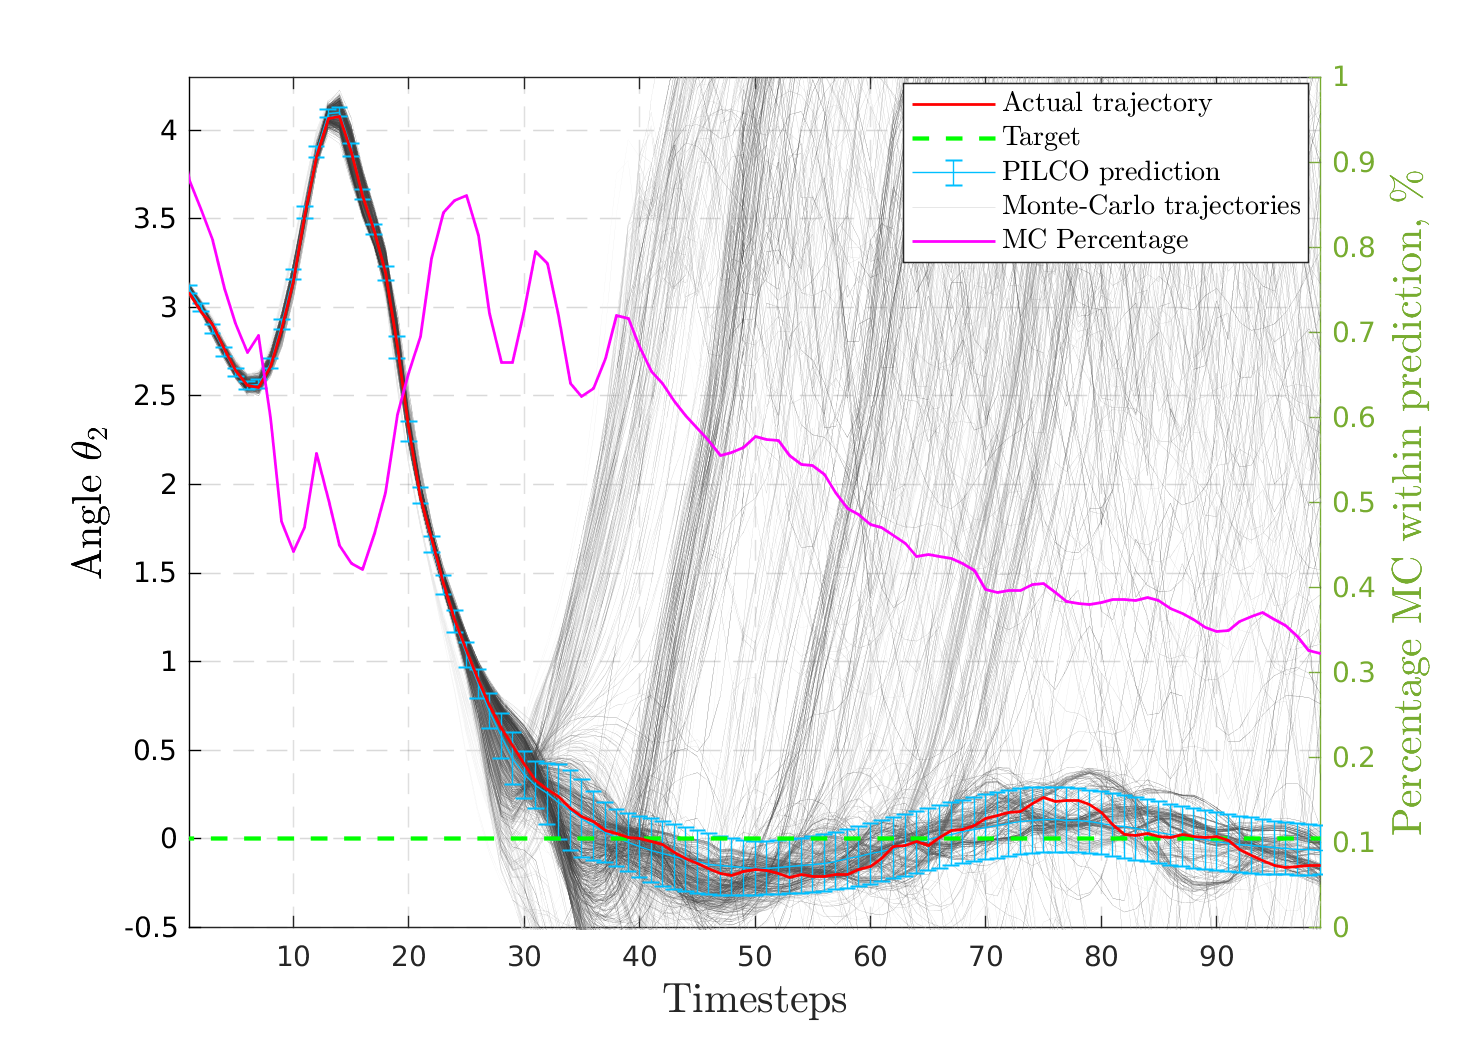
\includegraphics[height=0.4\textheight,width=1\textwidth]{Chapter3/Figures/cdp_MC_rollout_Ep_80_Dim_5.png} 
    \caption{Pendulum angle $\theta_2$ (rad)} 
    \label{Fig:Re-cdp-angle2} 
  \end{subfigure}
  \hspace{\fill}
  \begin{subfigure}[b]{1\linewidth}
    \centering
    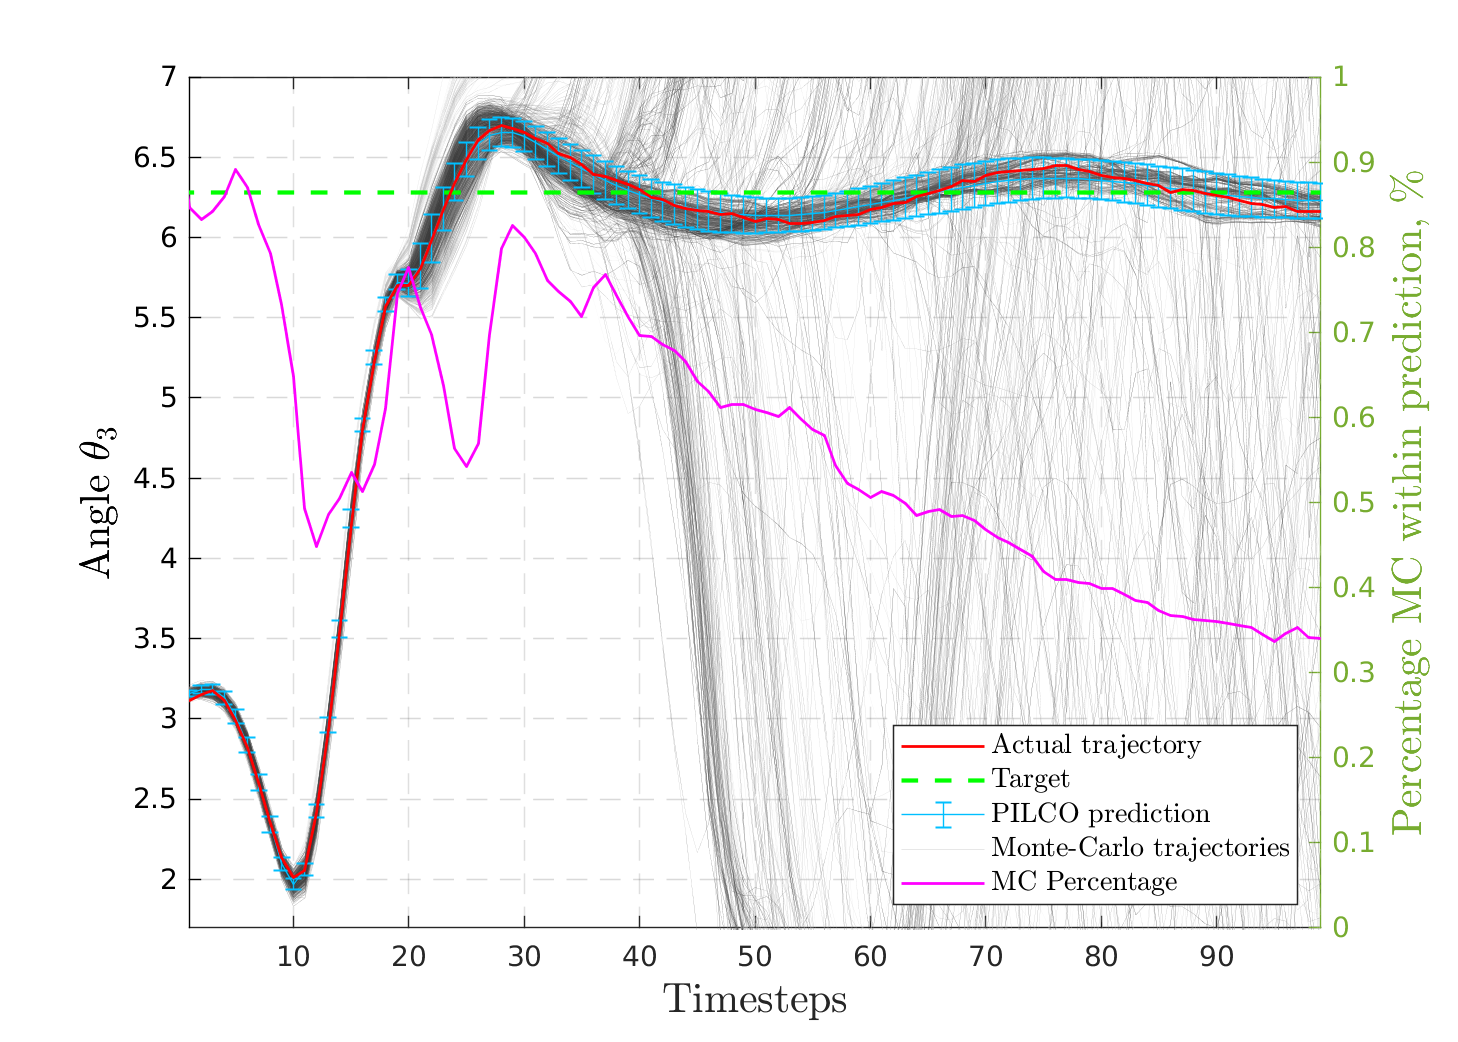
\includegraphics[height=0.4\textheight,width=1\textwidth]{Chapter3/Figures/cdp_MC_rollout_Ep_80_Dim_6.png} 
    \caption{Pendulum angle $\theta_3$ (rad)} 
    \label{Fig:Re-cdp-angle3} 
  \end{subfigure} 
\caption[Monte Carlo roll-outs for \textbf{cart-double-pendulum} pendulum angles]{Monte Carlo roll-outs for the \textbf{cart-double-pendulum} environment for  pendulum angles]. Figures show a random sample of the Monte Carlo trajectories for episode 75. The first three legend items (actual trajectory, target, PILCO prediction and MC trajectories) correspond to the state variable axis (left axis) and the magenta line shows the percentage of MC trajectories inside PILCO's prediction (2 standard deviations) (right axis). Sample time 0.05s, roll-out horizon 5.0s.}
\label{Fig:Re-cdp-MC-roll-outs-3} 
\end{figure} 
 
 
\begin{figure}[htbp]    
  \begin{subfigure}[b]{1\linewidth}
    \centering
    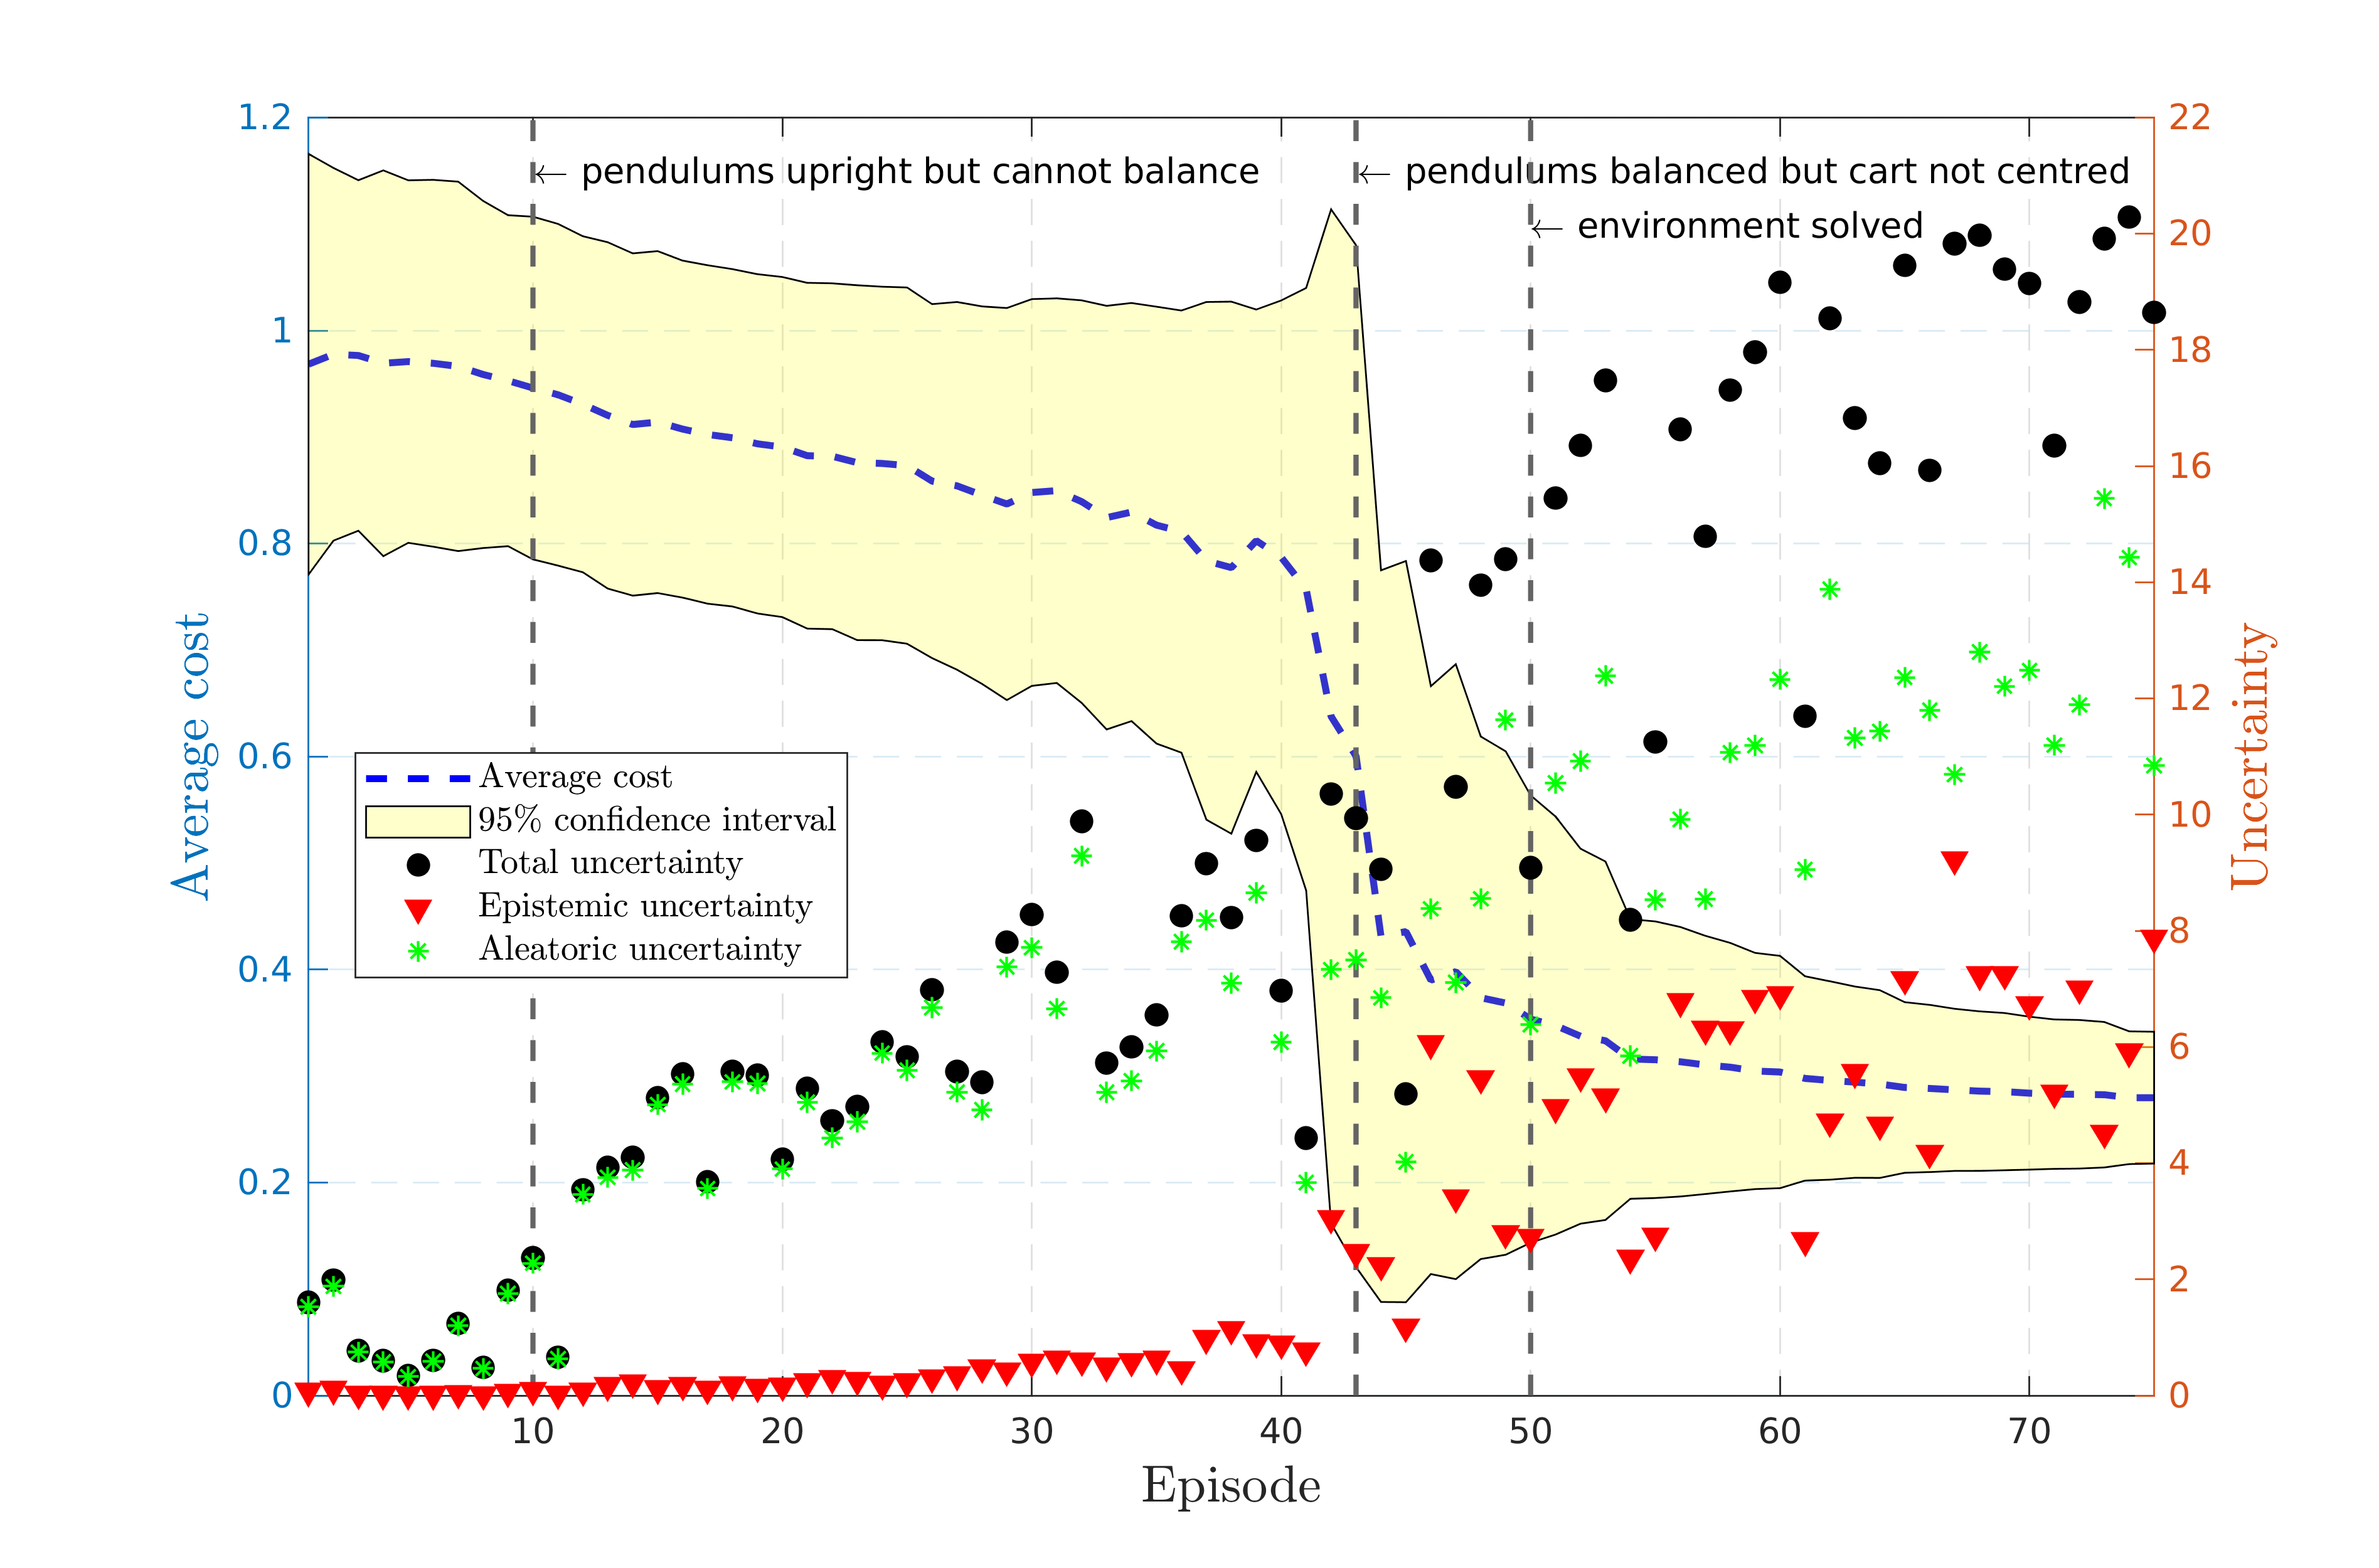
\includegraphics[height=0.4\textheight,width=1\textwidth]{Chapter3/Figures/cdp_uncertainty.png}
    \caption{Average cost (left axis) and uncertainty decomposition (right axis) for each episode over the course of learning.} 
    \label{Fig:Re-cdp-uncertainty} 
  \end{subfigure} 
  \begin{subfigure}[b]{1\linewidth}
    \centering
    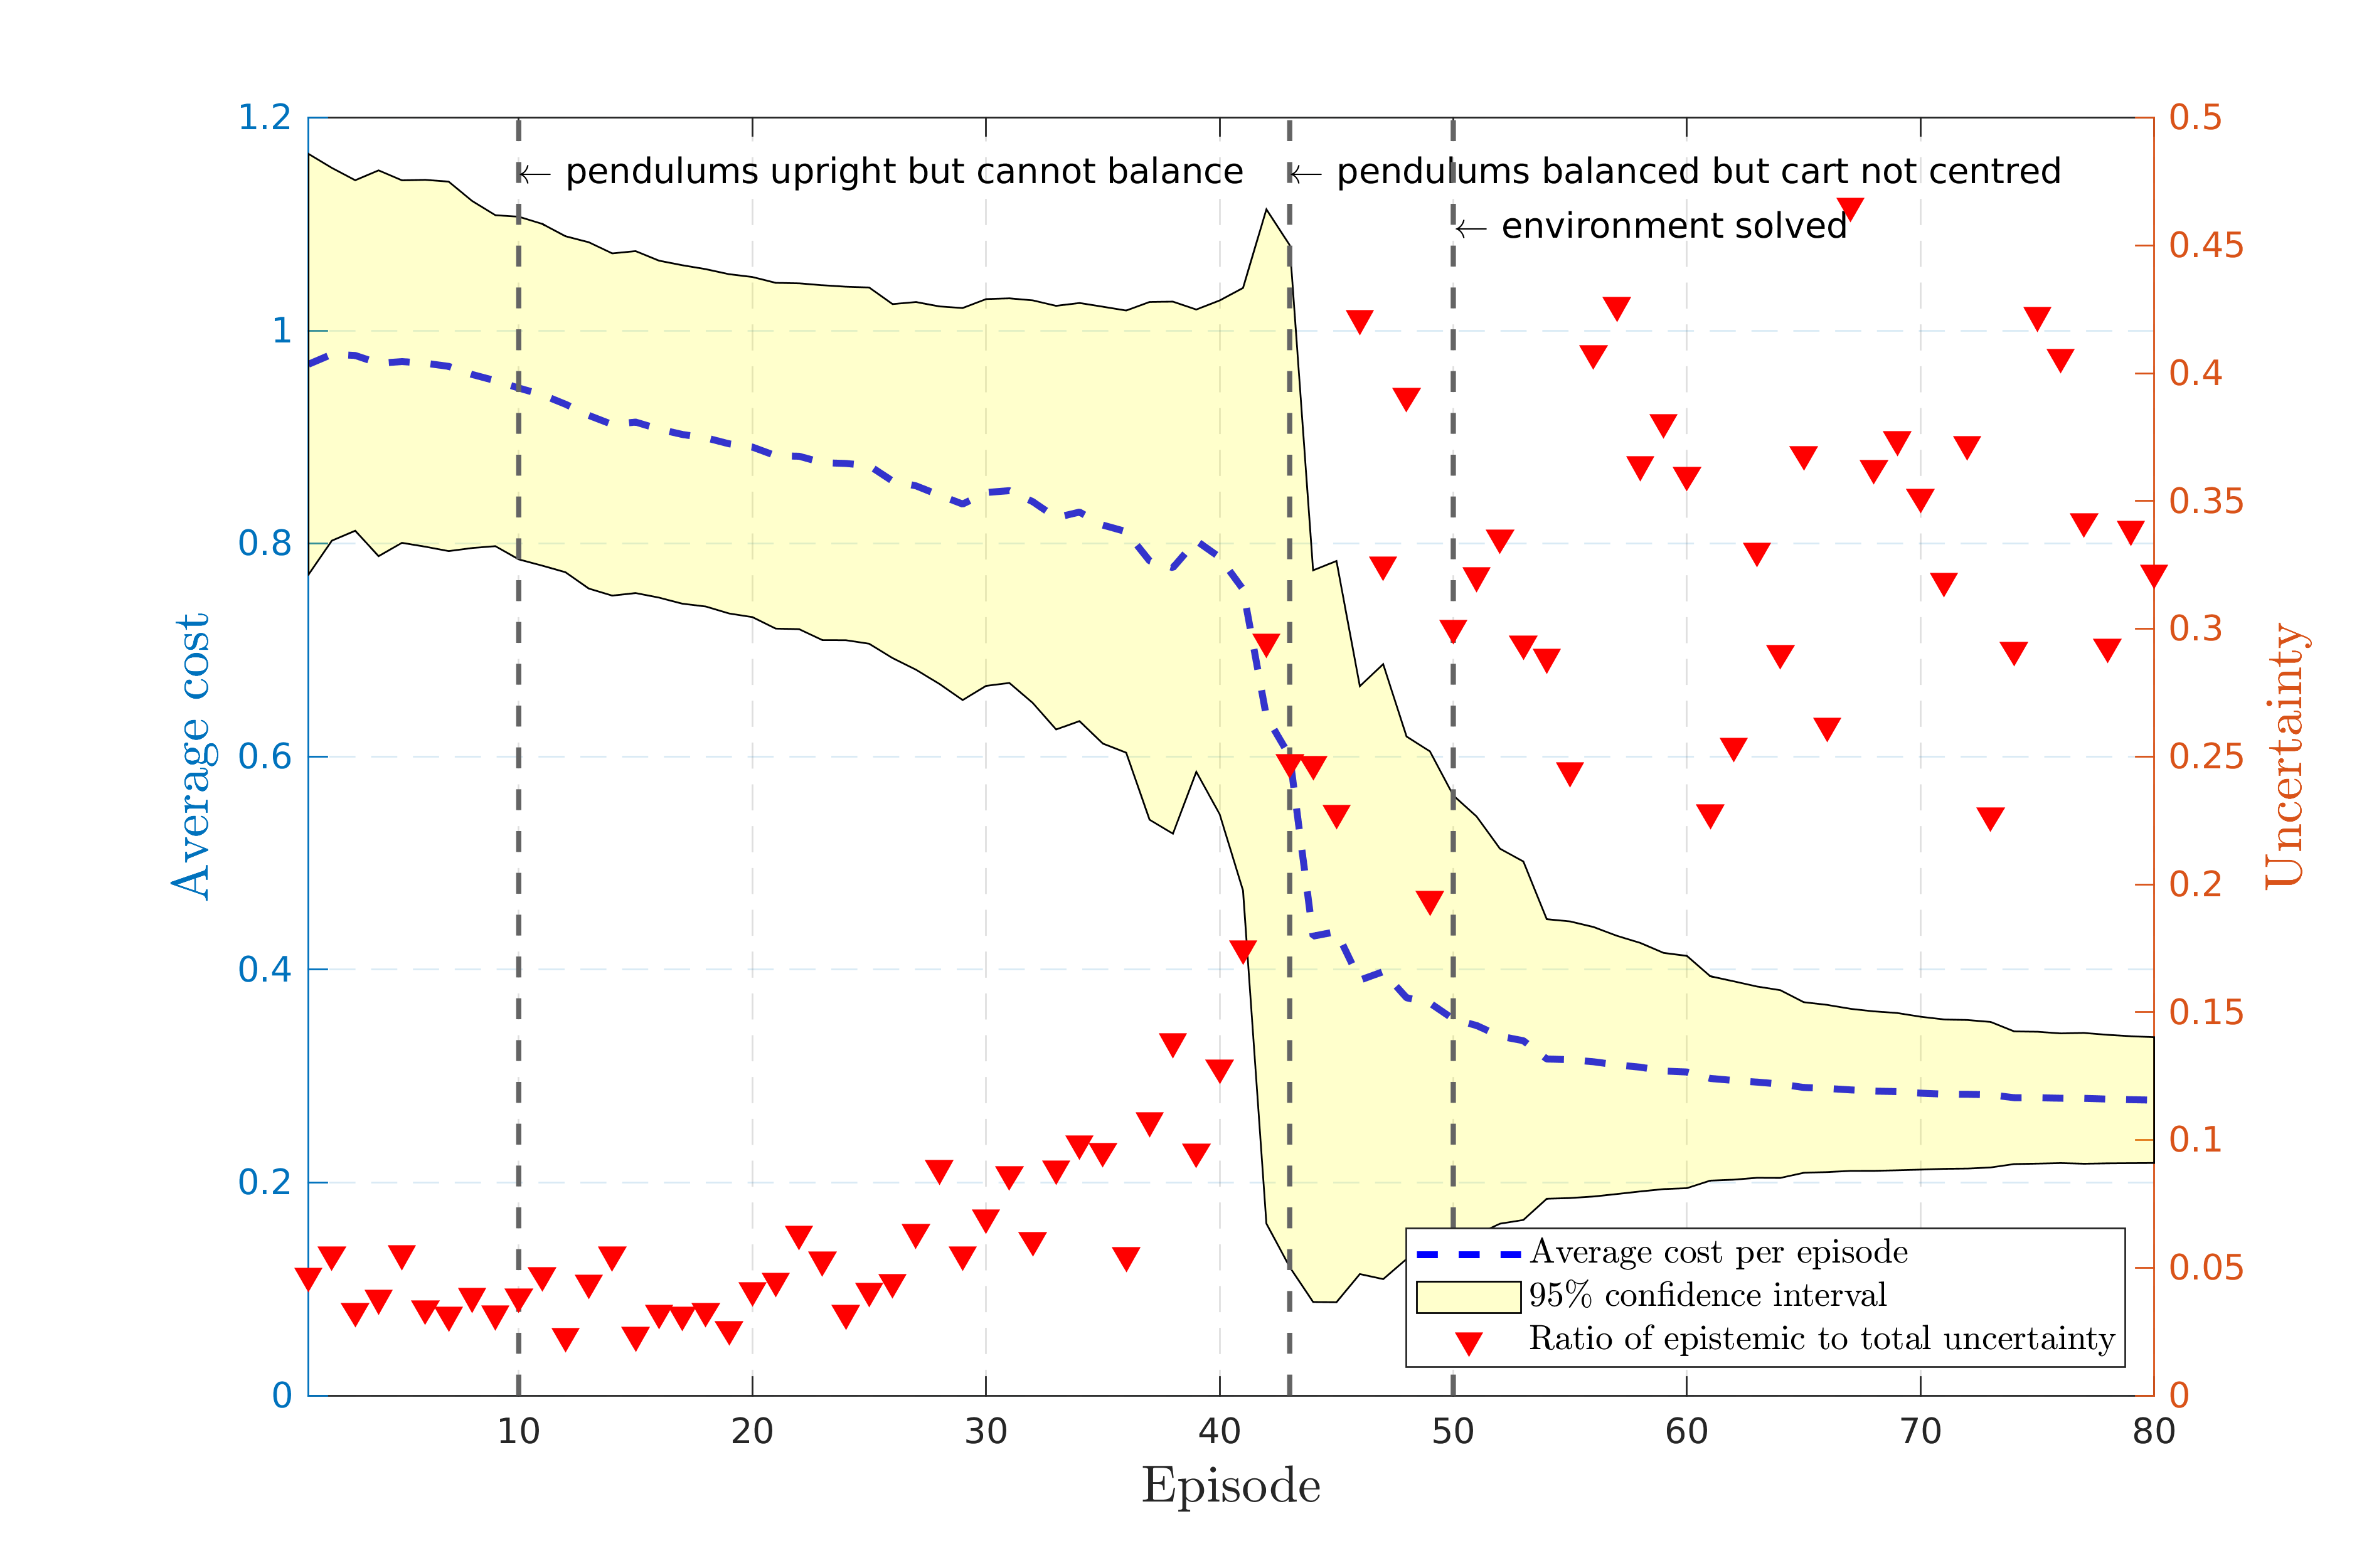
\includegraphics[height=0.4\textheight,width=1\textwidth]{Chapter3/Figures/cdp_uncertainty_normalised.png} 
    \caption{Average cost (left axis) and ratio of epistemic to total uncertainty (right axis) for each episode over the course of learning.} 
    \label{Fig:Re-cdp-uncertainty-normalised} 
  \end{subfigure} 
\caption[Uncertainty decomposition for \textbf{cart-double-pole} environment]{\textbf{Cart-double-pole}: Average cost (left axis) and uncertainty (right axis) for each episode over the course of learning.}
\label{Fig:Re-cdp-full-uncertainty} 
\end{figure}

\section{Discussion}
\label{S:Discussion}
The results in section \ref{S:Re-PILCO-envs} demonstrate that there is a clear correlation between the ratio of epistemic to total cost uncertainty under a given policy $\pi$ and the rate of PILCO's learning. Policies with higher ratios of epistemic to total cost uncertainty resulted in more efficient learning and policies with lower ratios learned more slowly. The ratio of epistemic and total cost uncertainties is an interesting metric which takes into account both the aleatoric and epistemic uncertainty values and provides a relativistic summary of cost uncertainty for a given policy. The result for the Pendubot environment (Fig. \ref{Fig:Re-pen-full-uncertainty}) that considered the ratio of epistemic to total cost uncertainty successfully highlighted policies that lead to large step decreases in average cost which were harder to interpret when only taking either the epistemic or aleatoric components into account. For example, in Fig. \ref{Fig:Re-pen-uncertainty} the epistemic cost uncertainty for the policies in episodes 8 and 9 are similar but when viewed as a ratio the policy associated with episode 8 is highlighted as that which has a larger impact on learning. 

For the cart-double-pendulum environment it is more difficult to pin-point examples where the ratio of epistemic to total cost uncertainty clearly highlights which of two similar epistemic or aleatoric cost uncertainty values has greater impact on learning, as was done the pendubot environment. This could be because cart-double-pendulum is significantly more complex than the pendubot. There is still, however, a pronounced correlation between the ratio of epistemic to total cost uncertainty and the rate of learning (Fig. \ref{Fig:Re-cdp-full-uncertainty}). Although the cart-double-pendulum simulation was only run for 80 episodes due to time constraints, one would expect that the ratio of epistemic to total uncertainty would begin to decrease with more episodes as the policy becomes refined and the model gains more confidence, as was the case for the pendubot environment.

For the cart-double-pendulum environment (Fig. \ref{Fig:Re-cdp-full-uncertainty}) PILCO learns to swing the pendulums to the upright position in 10 episodes but then takes a further 33 to learn to maintain them in a balanced state. Indeed, the act of balancing the pendulums is a significantly harder problem to solve than swinging them into position. During this phase the learning rate is slow which is indicative of the absence of an exploration scheme. PILCO always exploits the policy associated with the minimum expected long-term cost which leads to the agent being overly conservative in complex environments where exploration is required to properly explore the state-space. In this setting, the use of the saturating cost function initiates a natural exploration phase where the policy seeks out uncertain states. This is because an unexplored region of the state space with a wide state distribution is more likely to have substantial tails that extend into a low-cost region than a more peaked distribution. However, the gentle learning gradient during this period indicates that learning is not taking place in an efficient manner and highlights the need for an active-exploration algorithm. Future work could incorporate the Monte Carlo method presented in Section \ref{S:monte-carlo-estimate} into an objective function to create a balance between cost and the ratio of epistemic to total cost uncertainty. The objective could then be tuned to either seek policies with higher or lower ratios of epistemic to total cost uncertainty and the effect on learning efficiency could be examined.

\subsubsection{A closer look at propagating uncertainties:}
The approximating model predictive variance in Eq. \ref{Eq:Model-predictive-variance} has two terms; one representing the noise on the target data and the other, the uncertainty over of the model parameters. One might incorrectly assume that the uncertainty decomposition presented in Eq. \ref{Eq:uncertainty-decomposition} could be estimated in a simpler way by separately accumulating the terms of Eq. \ref{Eq:Model-predictive-variance} each time a step is taken through the transition function to get estimates of the aleatoric and epistemic uncertainties in the transition function. The following sources of uncertainty need to be considered: 

% However, different sources of uncertainty propagate through the model in different ways.
\paragraph{Observation noise:} A source of aleatoric uncertainty is the observation noise. For example, the transition function is really noise free but because the equipment has a measurement tolerance it cannot reveal the true value of the transition. The equipment will never be able to reveal the true state values but if a distribution is propagated through the predictive distribution the model may be able to predict the true state. 

\paragraph{Process noise:} A further source of aleatoric uncertainty is process noise. This accounts for uncertainties that are inherent in the dynamics of the system which mean that you cannot predict the state exactly. These could arise when not all parts of the system are measured. For example, friction that changes as a function of heat.

\paragraph{Parameter uncertainty:} The primary source of epistemic uncertainty in model-based reinforcement learning is parameter uncertainty which is reduced with the observation of more data.

Interestingly, all three types of uncertainty propagate forward through the model in different ways. In general, observation noise is irrelevant because the model can get around this by gaining access to repeated measurements. Whereas the model does not necessarily know how to deal with process noise. Since PILCO uses a GP model, it makes sense to consider the process in terms of a GP model. GP's are good at modelling observation noise but it is complicated to deal with noise present on the inputs. The reason for this is that a GP is completely defined by a mean and covariance function and the predictive distribution depends on the inverse of the covariance matrix. So building in uncertainty into the entries of the covariance matrix and then inverting it has influences throughout the model. PILCO gets around this issue by training on the difference between noisy observations, and then recognising that one source of noise on the data comes from input noise and the other from observation noise so the noise variance is approximately double and so is divided by two.

When propagating uncertainty through the transition function, all the different types of uncertainties and the way they propagate forward need to be considered, which becomes complex. So simply accumulating the the two different terms as proposed for an uncertainty would not provide a realistic estimate of the aleatoric and epistemic uncertainties in the transitions. In particular because at each step forward the total input variance must be considered in order to guarantee that the propagation spans all eventualities about the way the uncertainty propagates.


\section{Conclusion}
\label{S:conclusions}
In this dissertation I investigate how PILCO uses uncertainty in its decision making process. I show that when PILCO is learning efficiently it is selecting policies associated with a high ratio of epistemic cost uncertainty to total cost uncertainty. In contrast, when learning is slow PILCO is selecting policies associated with a low ratio of epistemic cost uncertainty to total cost uncertainty. 

To do this, I disentangle and quantify the different sources of uncertainty in a model that approximates PILCO's transition function. Since PILCO is a direct policy search method, it directly consults the cost function; therefore, I examine the influence of the uncertainty present in the transition function on uncertainty in the cost. I use variance as a metric to quantify uncertainty and use the law of total variance to decompose the uncertainty in the cost into aleatoric uncertainty and epistemic uncertainty. I introduce a gold-standard Monte Carlo scheme to separately estimate the aleatoric and epistemic uncertainties present in the cost by propagating trajectories through an approximation to PILCO's dynamics model. 

PILCO evaluates a particular policy by cascading uncertain inputs through its probabilistic GP dynamics model. It does this to gain insight into the variety of states that could be encountered and uses this information to search for a low cost policy. This approach only allows PILCO to make decisions based on the total uncertainty quantified by the model's predictive distribution, when there are in fact both aleatoric uncertainty and epistemic uncertainty components present in the model. This means that PILCO could be exploring regions in the state space that are irrelevant for the task of learning control because it is making decisions based on the total uncertainty without knowledge of its constituents. 

Future work could incorporate the Monte Carlo estimation method into an objective function to create a balance between cost and the ratio of epistemic cost uncertainty to total cost uncertainty. The objective function could then be tuned by means of an adjustable hyperparameter so that the agent either focuses on seeking policies with higher or lower ratios of epistemic to total cost uncertainty and the effect on learning efficiency could be examined. The adjustable hyperparameter could be treated in a similar fashion to $\epsilon \text{-greedy}$ exploration mechanisms where the amount of exploration is adjusted to create different behavioural traits in the agent.



